% USC Dissertation/Thesis LaTeX Template
% Edited by Ruda Zhang, 2020-10-08.
% -----------------------------------------------------------------------------
%	PACKAGES AND DOCUMENT CONFIGURATION
%-----------------------------------------------------------------------------

% Use `report` class with `USCthesis` package (style file) by Brian P. Gerkey
% Font size should be 11 or 12 points for regular paragraph text.
\documentclass[letterpaper,12pt]{report}
% [options] can be any of these default/alternative flag:
%   dissertation/thesis, final/proposal, copyright/nocopyright,
%   fussy/sloppy, flushbottom/raggedbottom, clref/opref.
\usepackage[proposal]{USCthesis}

% Packages required by `USCthesis.sty`.
\usepackage{hyperref}
\usepackage{setspace}
\usepackage{tabularx}

% Line spacing and margins in compliance with USC graduate school guidelines.
\usepackage[margin=1in,footskip=.5in]{geometry}
\doublespacing

% Optional packages: mathematical fonts and symbols
% You may comment this section out if you don't need them.
\usepackage{mathptmx} % set font to Times Roman
\usepackage[OT1]{fontenc} % font encoding for xelatex
\usepackage{mathtools}
\usepackage{amsmath}
\usepackage{amssymb}

% Optional packages: graphics
\usepackage{graphicx}
% You can use the "demo" option while editing to avoid compiling figures.
% \usepackage[demo]{graphicx}
% You can add absolute paths as well.
\graphicspath{{./}{../}{figures/}{../figures/}}

% Optional packages: bibliography with BibLaTeX.
% Comment this section out if you prefer BibTeX.
\usepackage[
    style=nature,
    sorting=none,
    isbn=false,
    url=false,
    doi=true,
    eprint=false,
    date=year,
    maxnames=6,
    minnames=6
]{biblatex}
\usepackage{tcolorbox}
\AtEveryBibitem{\clearfield{eventtitle}} 
\AtEveryCitekey{\clearfield{eventtitle}}
\AtEveryBibitem{\clearfield{pagetotal}} 
\AtEveryCitekey{\clearfield{pagetotal}}
\addbibresource{references.bib}

% Filler text for formatting. Comment these lines out for real writing.
\usepackage[english]{babel}
\usepackage{blindtext}
\usepackage{subfig}
\usepackage{pifont}% http://ctan.org/pkg/pifont
\newcommand{\cmark}{\ding{51}}%
\newcommand{\xmark}{\ding{55}}%


\begin{document}

%-----------------------------------------------------------------------------
%	TITLE PAGE
%-----------------------------------------------------------------------------

% Volume name could be added as option, e.g. `[Volume I]`.
\title{\textbf{\Large{Contextual approaches for improved multimodal content understanding}}}

\author{Digbalay Bose}

% Committee list is only shown in `proposal` layout.
\committee{Prof.Shrikanth Narayanan & (Chair)\\*
           Prof. Antonio Ortega \\*
           Prof. C.C.Jay Kuo\\*
           Prof. Mahdi Soltanolkotabi\\*
           Prof. Jesse Thomason & (Outside Member)}

% Submission information is only shown in `final` layout.
\majorfield{Electrical and Computer Engineering}
\submitdate{September 2023}  % Must be one of the three dates allowed in the guideline

% Make sure everything, specially your title page, exactly follows the guideline:
% https://graduateschool.usc.edu/wp-content/uploads/2020/11/Manuscript_Formatting_and_Documentation_Styles.pdf

%-----------------------------------------------------------------------------
%	PREFACE
%-----------------------------------------------------------------------------

% The preface environment prints the title page.
\begin{preface}

  % Dedication Page, which is truly unnecessary.
  % \prefacesection[Dedication]{}
  % \input{dedication}

  % Acknowledgement Page, which is also unnecessary for proposals.
  % \prefacesection{Acknowledgements}
  % \input{acknowledgements}

  \tableofcontents
  \listoftables   % Comment this out if you don't have tables
  \listoffigures

  % Abstract Page
  \prefacesection{Abstract}
  
In today's information-rich landscape, there has been a rapid rise in content available through web-based platforms reliant on diverse modalities. Multimodal content can manifest in varied forms like online news articles, movies, advertisements, and digital short videos. Our ability to comprehend the underlying narratives in these sources depends on the integration of various modalities, including audio, visual, and language. Further proliferation of multimodal content across diverse platforms necessitates a large-scale understanding of its impact on individuals and society as a whole. 
\par
In this work, we consider the problem of multimodal content understanding at diverse scales to obtain a holistic view of the input sources. Further, our approach to content understanding is reliant on contextual information processing from multimodal input sources. We process diverse forms of contextual information through various modalities and integrate the same using context-guided attention mechanisms. We show that the inclusion of context information improves multi-scale content understanding across a variety of input sources like movies, advertisements, TV shows, and natural scene images. We further conclude by providing directions for future research where we would like to explore information theoretic approaches for extracting optimal representations from context-guided attention mechanisms.







\end{preface}

%-----------------------------------------------------------------------------
%	CONTENT STRUCTURE
%-----------------------------------------------------------------------------

% Better to separate LaTeX structure and content
\chapter{Introduction}
\label{cha:introduction}
This chapter provides the necessary background material and details the organization of my proposed work.

\section{Multi-modality}
\subsection{Modalities - Definition and Introduction}
\textit{Modality refers to the way something happens around us or is perceived by humans} \cite{Baltruaitis2017MultimodalML}. The world around us is composed of multiple sensory modalities, as listed below, with enabled capabilities:
\begin{itemize}
    \item \textbf{Visual:} Watching objects and events in the current visual scene
    \item \textbf{Language:} Verbal interactions with other humans 
    \item \textbf{Audio:} Speaking and hearing environmental sounds 
    \item \textbf{Touch:} Feeling texture of objects 
    \item \textbf{Smell:} Distinguishing between pleasant and unpleasant odors.
\end{itemize}
For humans, the information from multiple sensory sources is processed by distinct regions of the brain for different perceptual tasks \cite{Alain2001WhatA,BornkesselSchlesewsky2015NeurobiologicalRO,Wallace2002HistochemicalIO}. While the visual input processing is handled by the occipital lobe in the brain, the auditory and language inputs are processed by specific regions of the temporal lobe. The sub-division of the human neural processing system into regions that can process a wide variety of modalities indicates the heterogeneity among different sources along with underlying commonalities, as shown in Fig \ref{cerebral_cortex_modalities}.

\begin{figure}
    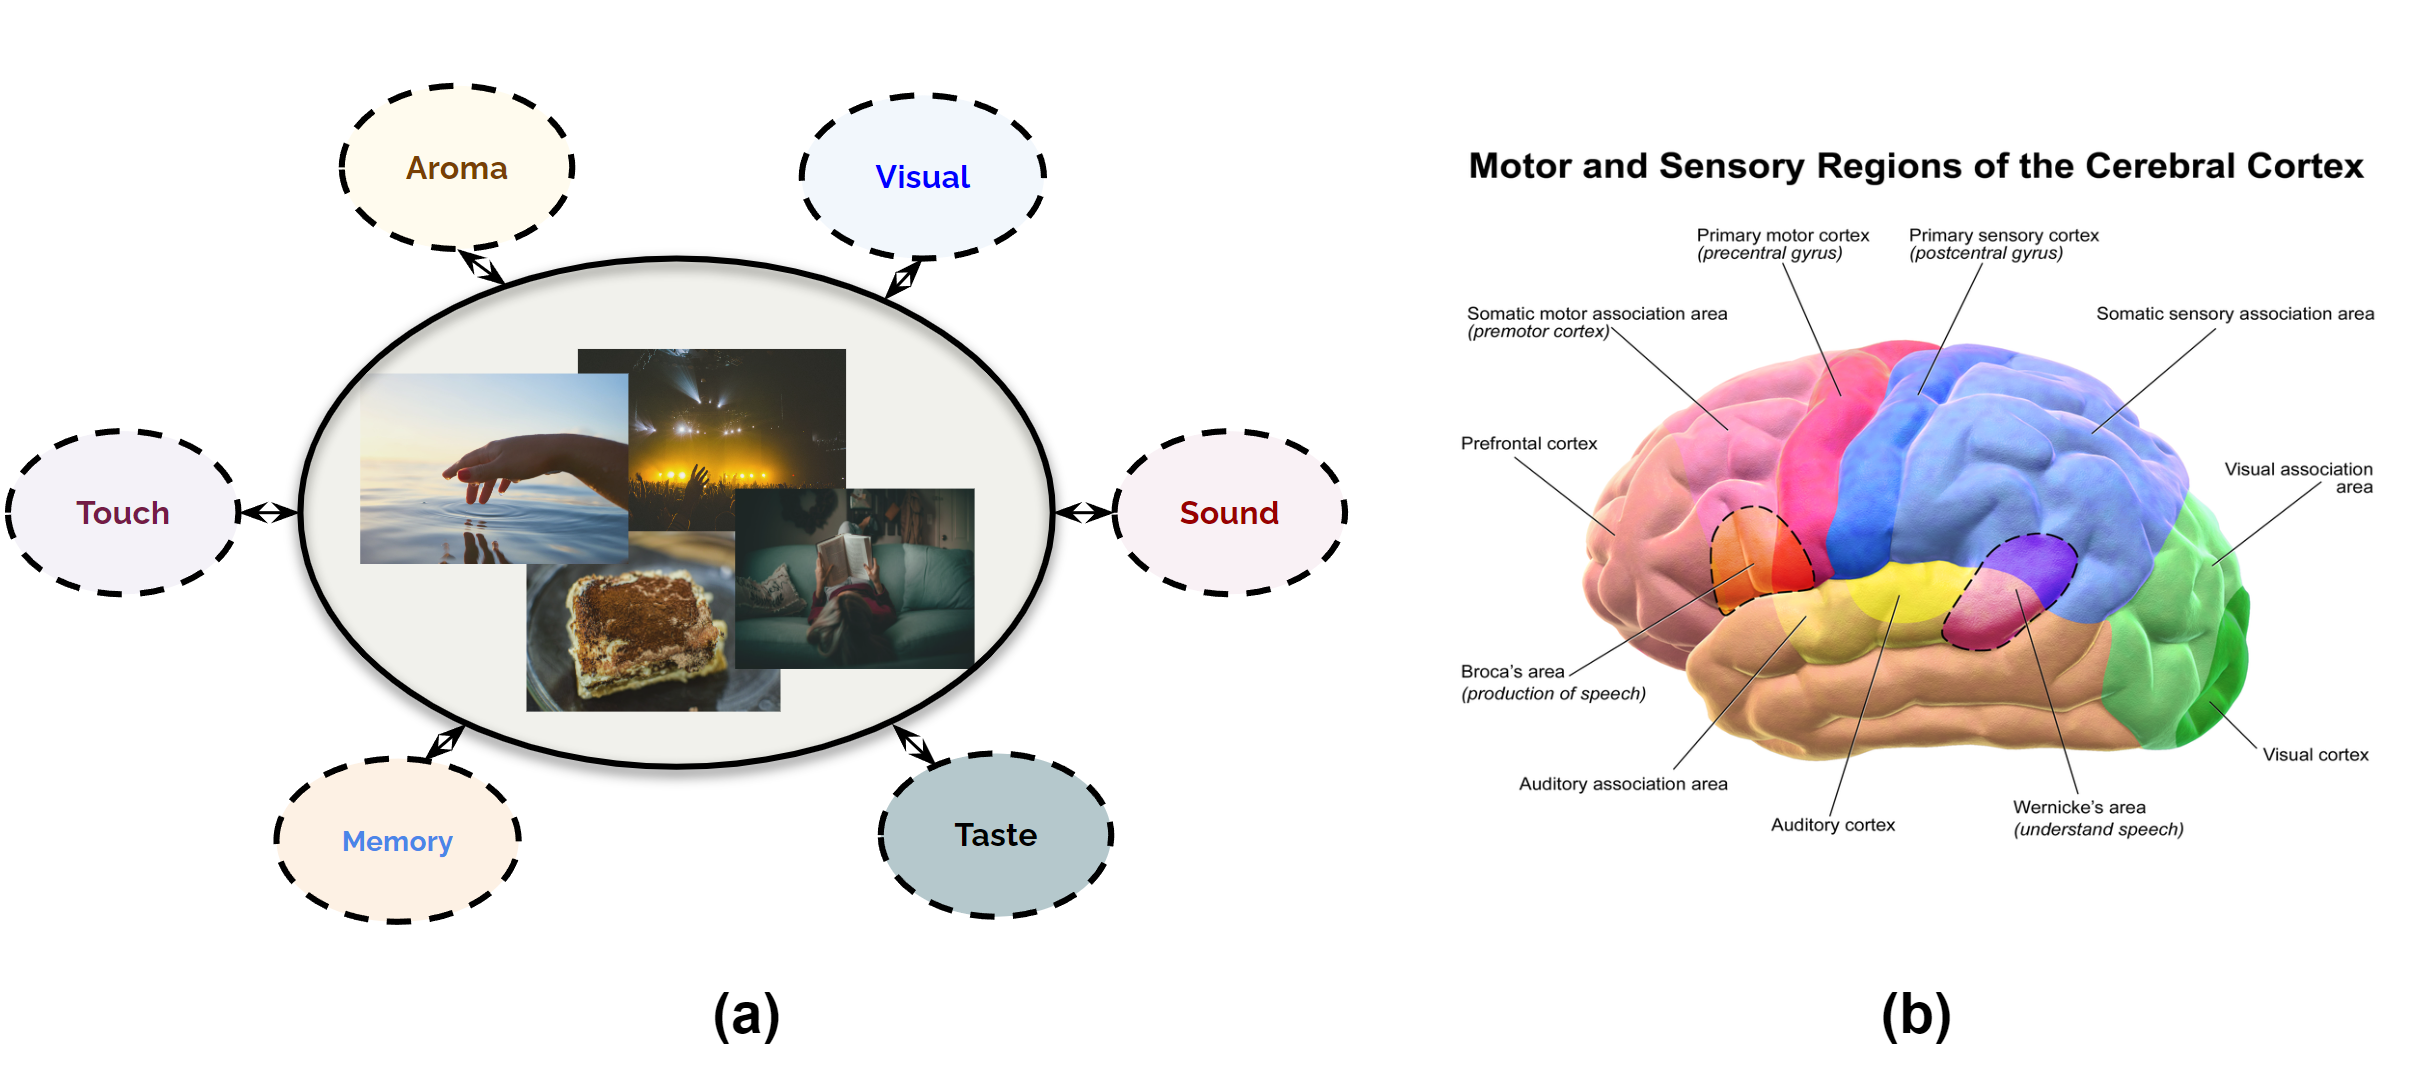
\includegraphics[width=\textwidth]{figures/cererbral_cortex_multiple_modalities.png}
    \caption{ (a)  Sensory modalities associated with real-world human perception  (b)  Specialized regions in brain where sensory information comes together and processed by different cortices}
    \label{cerebral_cortex_modalities}
\end{figure}

In artificial intelligence, a given task is considered multi-modal if multiple sensory modalities are needed to solve the same. The goal of artificial intelligence is to develop autonomous agents that can learn from diverse input modalities to solve complex reasoning tasks. As mentioned by Liang et al. \cite{Liang2022FoundationsAR}, the key properties associated with learning from multimodal data are listed as follows:
\begin{itemize}
    \item \textbf{Heterogeneity:} Heterogeneous nature of different modalities due to diversity in qualities, structures, and representations
    \item \textbf{Connectedness:} Shared/common information between different modalities due to inter-related nature.
    \item \textbf{Interaction:} Existence of optimal interactions/fusions between different modalities, suitable for particular task.
\end{itemize}
Based on the above properties associated with multiple modalities, the major challenges in multimodal learning \cite{Liang2022FoundationsAR} can be summarized below:

\begin{itemize}
    \item \textbf{Representation:} Learning representations through fusion mechanisms that capture the heterogeneity of the modalities along with the shared information. For example, language is considered symbolic due to its word-based composition, whereas audio and visual modalities are represented through signals.
    \item \textbf{Alignment:} Identifying relationships between (sub) elements of different modalities. This requires similarity computation between different modalities along with the handling of long-term dependencies.
    \item \textbf{Reasoning:} Combining knowledge from multiple sources (including external, i.e. knowledge graphs) in a multi-step inference process by exploiting the task structure.
    \item \textbf{Generation:} Translating between different modalities and summarization of multimodal data by preserving the salient content.
    \item \textbf{Transference:} Transferring cross-modal knowledge from secondary modalities to the primary modality in the presence of noise or limited data.
\end{itemize}

% In this work, we deal with the alignment, reasoning, and transference challenges associated with multi-modal learning.
    
\subsection{Rise of multi-modal content}

With the rapid rise in heterogeneous internet networks across the globe, vast amounts of web-based content have been generated at different scales, variety, and velocity \cite{Gao2020ASO}. Web-based sources convey information to the viewers through a combination of multiple modalities. For example, an online news article about a major sports event contains text descriptions with accompanying images. Further, the movies or TV shows hosted through online streaming platforms portray narratives through the combination of video and audio signals (music, speech, ambient sounds). 
The demand for media content, especially movies, TV shows, and advertisements, is expected to rise over the next three years, with the projected market value to reach 2.9 trillion US dollars, as shown in Fig \ref{media industry demand}.
\begin{figure}[h!]
    \centering 
     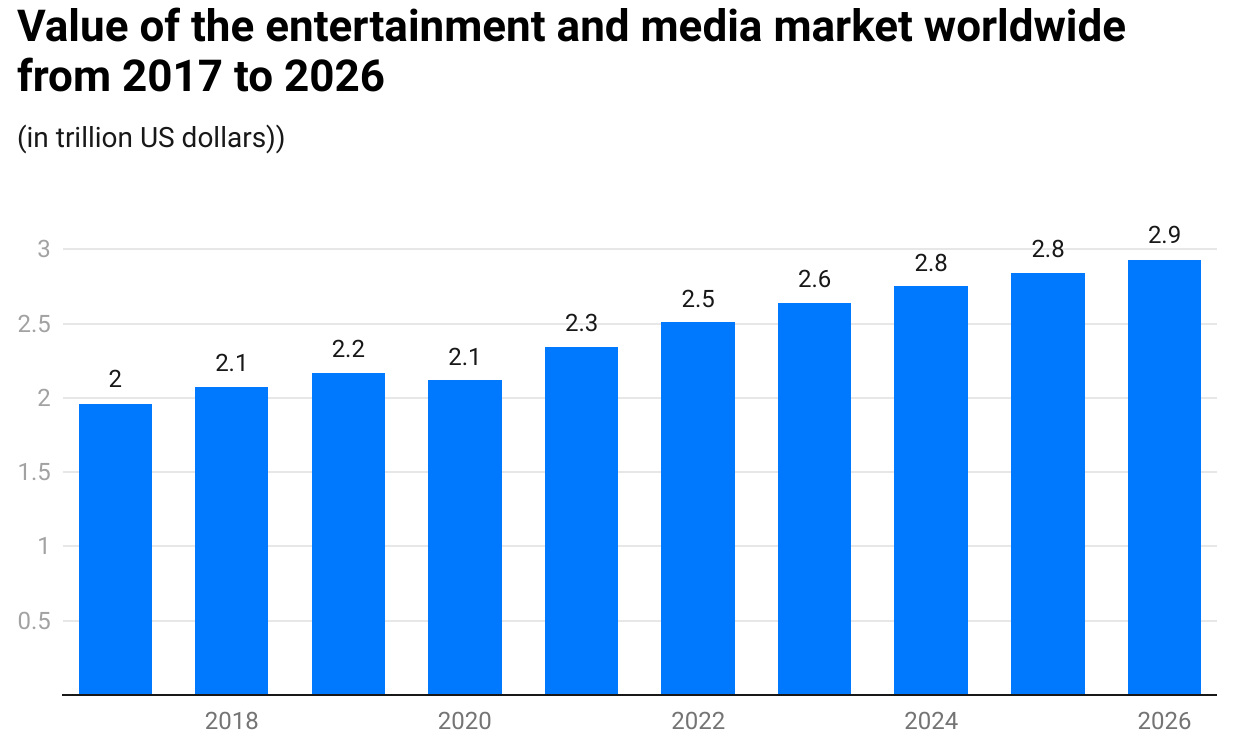
\includegraphics[width=0.6\linewidth]{figures/media_industry_demand.png}
     \caption[Media value]{Expected value of entertainment market industry from 2017 to 2026 \footnotemark} 
     \label{media industry demand}
\end{figure}
\footnotetext{\url{https://www.enterpriseappstoday.com/stats/media-and-entertainment-industry-statistics.html}}
The growing demand for multi-modal media content has led to various descriptive tasks such as captioning \cite{Abdar2023ARO}, video summarization \cite{Apostolidis2021VideoSU}, and question-answering \cite{defaria2023visual}, aimed at enhancing user experience. In the following sections we will introduce the concept of context and how multiple modalities provide contextual information.

\section{What is context ?}
In computer vision, context \cite{contextvision} refers to any relevant information encompassing the attributes of the object and event considered, along with other entities (objects and events) in the given scene, both visual and non-visual. Contextual information enables a wide variety of tasks, including object recognition, human affect perception, and salient event detection in videos, by providing additional cues needed for accurate inference. For example, the visual scene in a given image provides the necessary contextual information to detect commonly co-occurring objects along with any atypical placements. In terms of object placements, utensils are more likely to be found in the kitchen as compared to bedrooms or stadiums. An example of context providing the required information to improve object recognition under challenging conditions (poor lighting, image blurring, ) is shown in Fig \ref{object recognition}. The blurred object (marked by a red circle), when viewed in isolation, is not recognizable. However, when the object is placed in the context of the entire visual scene i.e. office, we can see that it is likely to be a keyboard.
\begin{figure}[h!]
    \centering 
     
\includegraphics[width=0.6\linewidth]{figures/blurred_object.png}
     \caption{ \textbf{LEFT:} A blurred object (marked in red circle), when viewed in isolation, is not recognizable. \textbf{RIGHT:} Contextual information in the form of the visual scene helps in recognition. Image source: \cite{Marques2010ContextMI}}
     \label{object recognition}
\end{figure}

Context also refers to the situation surrounding our responses and actions \cite{baez2018does}. An example of situational context can be seen in Fig \ref{context situation}. When the face is only considered, it conveys pain. However, by taking the entire situation into context involving the celebration, it can be inferred that the person is happy based on bodily expressions and the event (sports match). 

\begin{figure}[h!]
    \centering 
    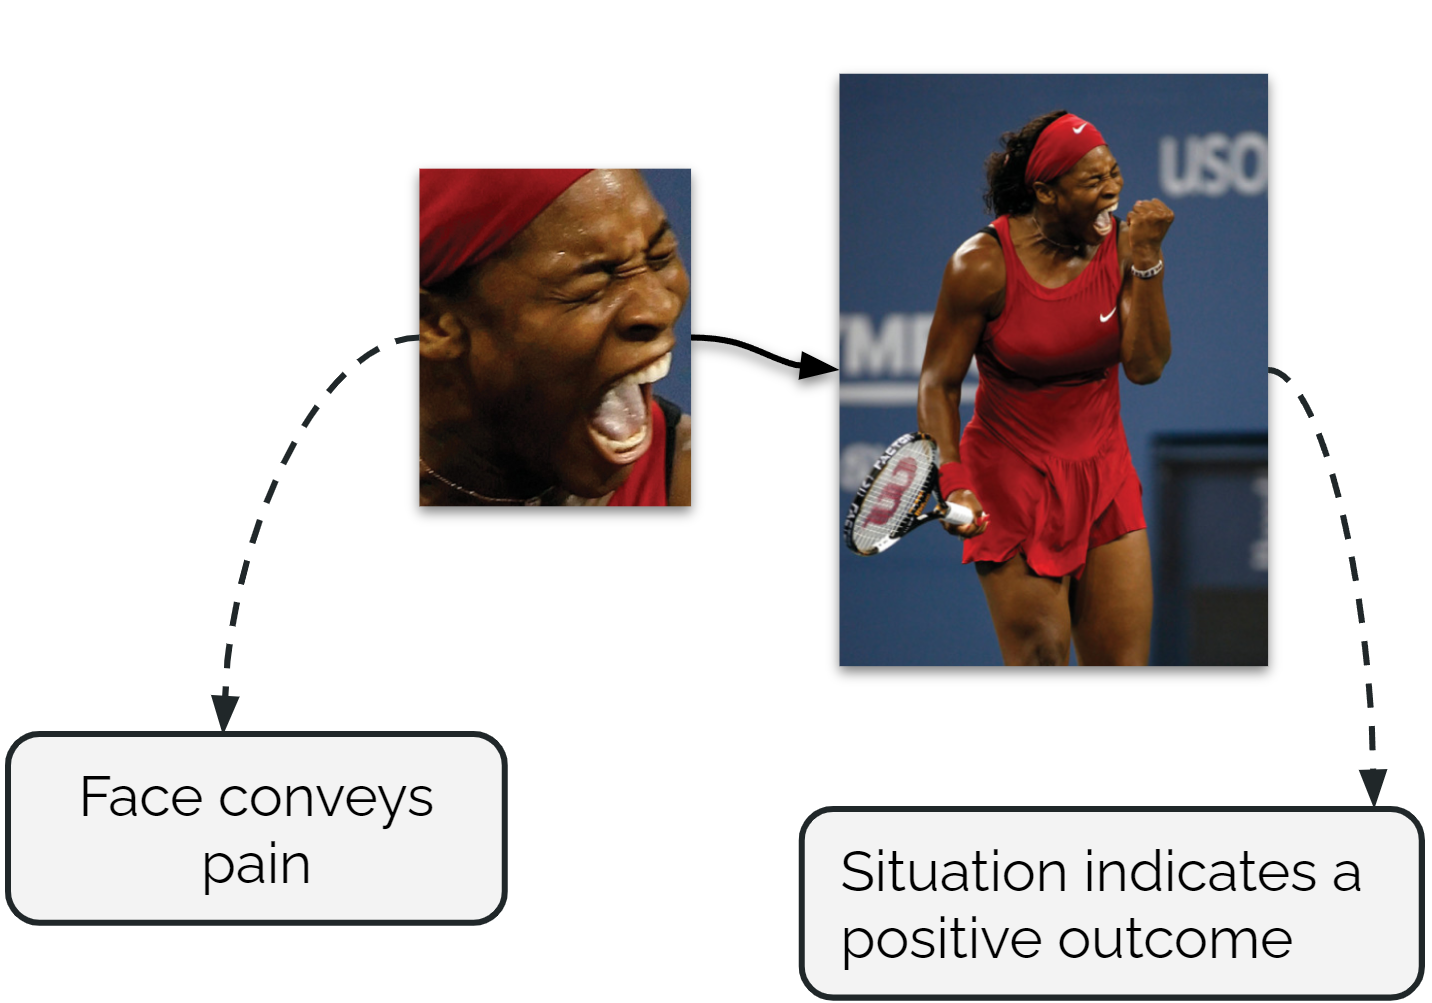
\includegraphics[width=0.6\linewidth]{figures/context_situation.png}
    \caption{Example of the situation as context information. Image source: \cite{barrettcontext} }
    \label{context situation}
\end{figure}


The broad organization of different context sources, along with associated levels is shown in Fig \ref{Context_type}.
\begin{figure}[t]
  \centering
  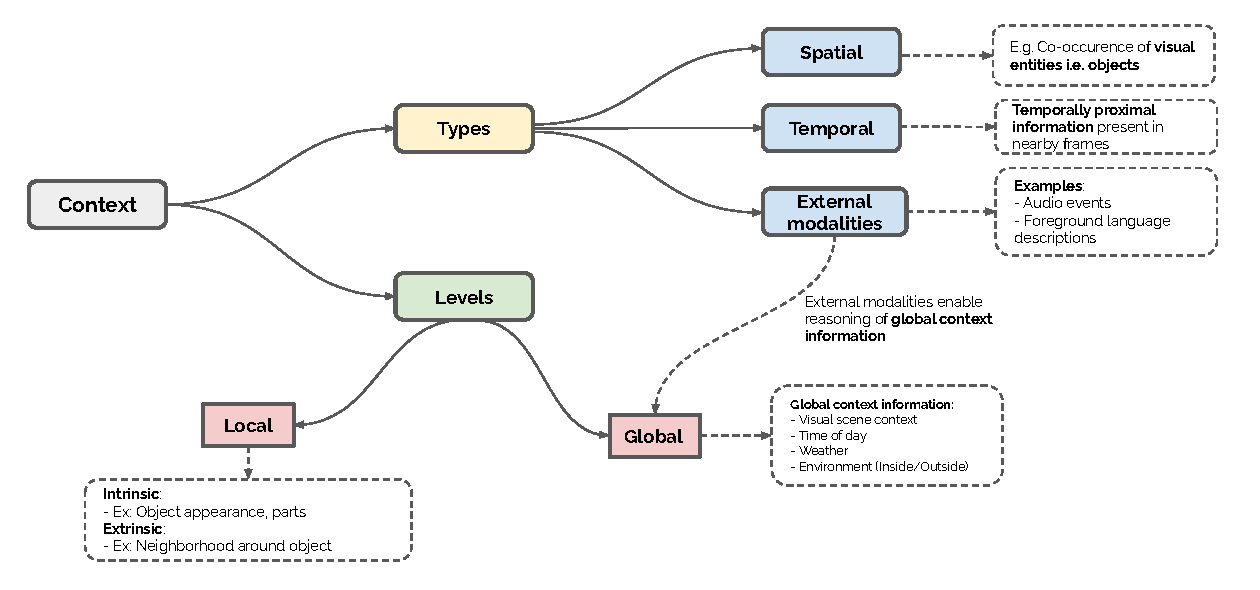
\includegraphics[width=\linewidth]{figures/Context_type.pdf}
  \caption{Variations in types and levels of context. Outline of context levels and types inspired from Fig 5 in \cite{contextvision}.}
  \label{Context_type}
\end{figure}
Context can be broadly divided into three types as follows:

\subsection{Spatial context}
Spatial context refers can be defined as the \textit{possibility of finding objects located at certain positions in the scene w.r.t other proximal objects}. For example, a ship can be found floating at sea rather than on a highway.
Spatial context can be further subdivided into the following major classes:
\begin{itemize}
    \item  \textbf{Spatial co-occurrence}: Spatial co-occurrence can be leveraged through co-occurrences of object labels in the same visual scene. Rabinovich et.al \cite{Rabinovich2007ObjectsIC} utilized co-occurrence statistics between labels in a CRF-based framework to refine object detections in a given visual scene. Further, Wang et al. \cite{Wang2007ShapeAA} expanded the idea of co-occurrence by providing a probability distribution of labels over different regions based on a given pixel location. Yang et.al \cite{Faceness-Net} explored fine-grained relative spatial information between facial parts i.e., placement of nose, mouth for face detection. 
    \item  \textbf{Direction and toplogical relations}: 2-D spatial relations between entities can be described through direction and topological-based relations \cite{Marques2010ContextMI}. Directional relations deal with the proximity of one object with other objects in terms of other entities based on relative terms like \textit{"near"}, \textit{"above"}, \textit{"below"}. Whereas topological relations are concerned with the neighborhood of the objects in terms of overlap/containment with distinct regions i.e. exterior, boundary and interior.
    \item  \textbf{Semantic driven spatial context}: Semantic context restricts the space of possible spatial contextual relations in a given scene to a set of valid ones. The usage of semantic context between proximal objects enables correction of mislabeling in images \cite{Rabinovich2007ObjectsIC}, and accurate discovery of all possible valid relations between objects through scene graphs \cite{Chang2021ACS}. An example of a scene graph with entities and semantic relations obtained after message-passing operations \cite{Xu2017SceneGG} is shown in Fig \ref{scenegraph}.
    \begin{figure}[h!]
    \centering
        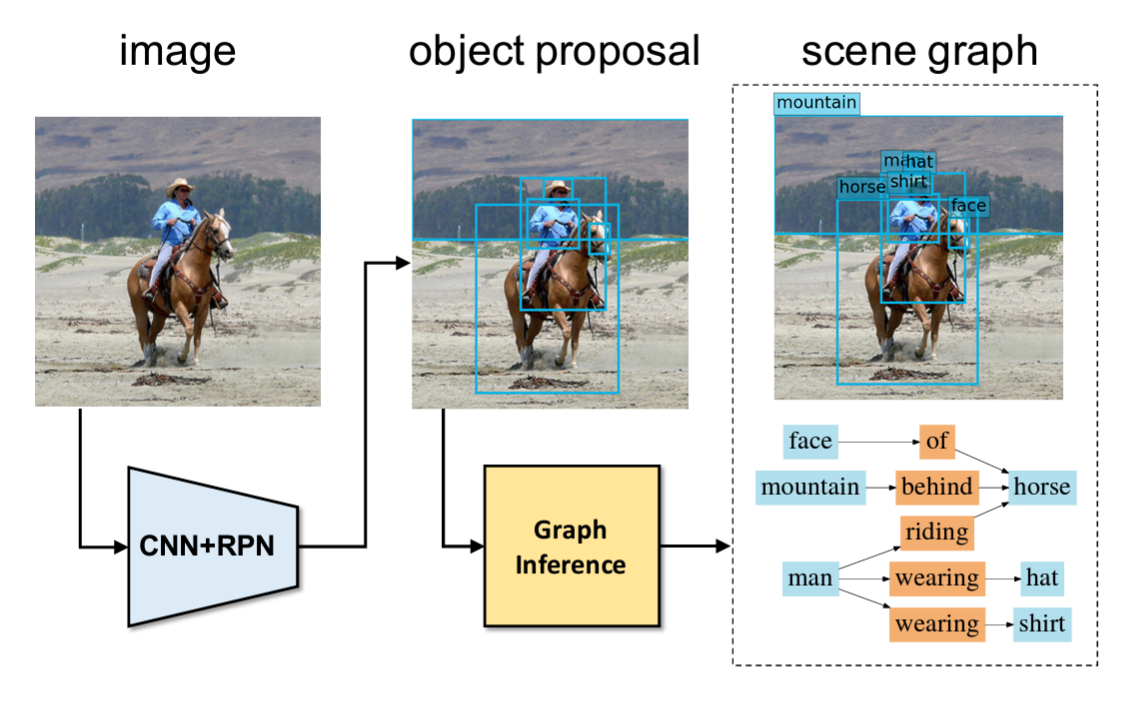
\includegraphics[width=0.5\linewidth]{figures/Scene_graph_outline.png}
        \caption{Sample scene graph obtained after iterative message passing (graph interface) over the region proposals (objects) }
        \label{scenegraph}
    \end{figure}
\end{itemize}

\subsection{Temporal context}
Temporal context refers to the \textit{information present in dynamic content, i.e. nearby or distant frames in videos}. The major subdivisions of temporal context are listed as follows:
\begin{itemize}
\item \textbf{Short-term temporal context:} Short-term temporal context relies on information present in nearby frames, which can be a short temporal window centered on the current frame or previous frame. The temporal context within a short window, (usually a few seconds) enables general video understanding tasks, including action recognition \cite{Carreira2017QuoVA}, pedestrian tracking \cite{Yan2019LearningCG}, human-object interaction \cite{Ji2021DetectingHR}. 
\item \textbf{Long-term temporal context:} Instead of limiting to nearby frames, long-term temporal context deals with temporal scale spanning from hours to months/years. General media-focused tasks based on movies \cite{Wu2021TowardsLV,Soldan2021MADAS} rely on long-form narratives (usually minutes to hours) for understanding character interactions, event dynamics, and broad semantics, including genre, etc. For tasks like species monitoring, temporal information over extended periods of time (months or years) is required for accurate identification \cite{Beery2019ContextRL}. 
\end{itemize}
In spite of clear divisions between short-term and long-term temporal contexts based on the duration of information, certain narrative-driven videos in media, i.e., advertisements, contain: 
\begin{itemize}
\item Rapid changes in short-term contextual information based on shots. 
\item Long-term contextual association between the shots based on an integrated narrative.
\end{itemize}
\subsection{External modalities}
Apart from visual-only information, modalities such as audio, language, and prior weather information also provide relevant contextual information for various reasoning tasks. For example, in the case of audio-visual tasks, the audio associated with an entity, i.e., dog barking, can help us estimate the proximity of the sound source and localize it in the given video \cite{Tian2018AudioVisualEL}. Further usage of audio modality as an additional contextual source for visual tasks has been explored in floorplan design \cite{purushwalkam2020audio} and audio-visual navigation for virtual agents \cite{chen2020soundspaces}. For various vision-language tasks like temporal grounding, natural language queries can be used as contextual inputs to isolate regions of interest in unconstrained videos \cite{Zhang2022TemporalSG}. Besides language and audio, additional contextual information available through thermal sensors \cite{Seymour2017AutomatedDA} is used to augment the visually captured data for improving wildlife detection in remote areas. In case of affect understanding problems, multi-turn dialogues (\textbf{language modality}) provide the necessary context information (i.e. topics and flow of information) along with facial expressions for emotion tracking of the speakers \cite{Zhao2022M3EDMM}.

\subsection{Local context}
Local context refers to the \textit{contextual information associated with objects itself (\textbf{intrinsic}) and surrounding local regions (\textbf{extrinsic}) such as color, shape, contrast, aspect ratio} \cite{contextvision}. Local context is closely related to spatial information in terms of the immediate neighborhood of the objects in the scene. Effective utilization of local context enables the detection of small objects in complex scenes with multiple entities. External modalities often provide local context for multi-modal reasoning, i.e., the conversation history (\textbf{language}) enables the autonomous agent associated with visual dialog \cite{Das2016VisualD} to provide the correct in-context answer.

\subsection{Global context}

Global context utilizes \textit{the overall configuration of the scene as a source of contextual information \cite{contextvision}}. The primary sources of global context information are as follows:
\textbf{(A) Visual scene:} The visual scene where the objects are present, i.e. living room, kitchen, train station etc. \\
\textbf{(B) Time of day:} The timing shown in the given image/video i.e. day, night, evening, or morning. \\
\textbf{ (C) Weather:} The ambient weather conditions associated with the given scene, i.e. sunny etc. \\
\textbf{ (D) Environment:} The environment associated with the given scene i.e., inside or outside.
\par 
Visual scene, along with the associated environment provides the prior context for finding certain objects. For example, there is a greater likelihood of finding utensils in the kitchen (\textbf{indoor visual scene}) as compared to train station (\textbf{outdoor visual scene}). Global context information (in the form of visual scenes) also influences the relative placement of different objects, like the proximity of a keyboard to the monitor in an office setup. Further, the accurate identification of different objects as part of the local contextual information in a given image/video can also help 
in recognizing the given visual scene \cite{Torralba2003ContextualPF} and its attributes (i.e., indoor/outdoor, time of day, etc.). For example, the presence of a microwave oven and dishwasher indicates that the visual scene is likely a kitchen. The global context information can also help in identifying atypical scenarios \cite{Choi2012ContextMA} involving objects i.e., a car located in the sky or a plane running on a highway, as shown in Fig \ref{outcontext}. 
\begin{figure}[h!]
    \centering
        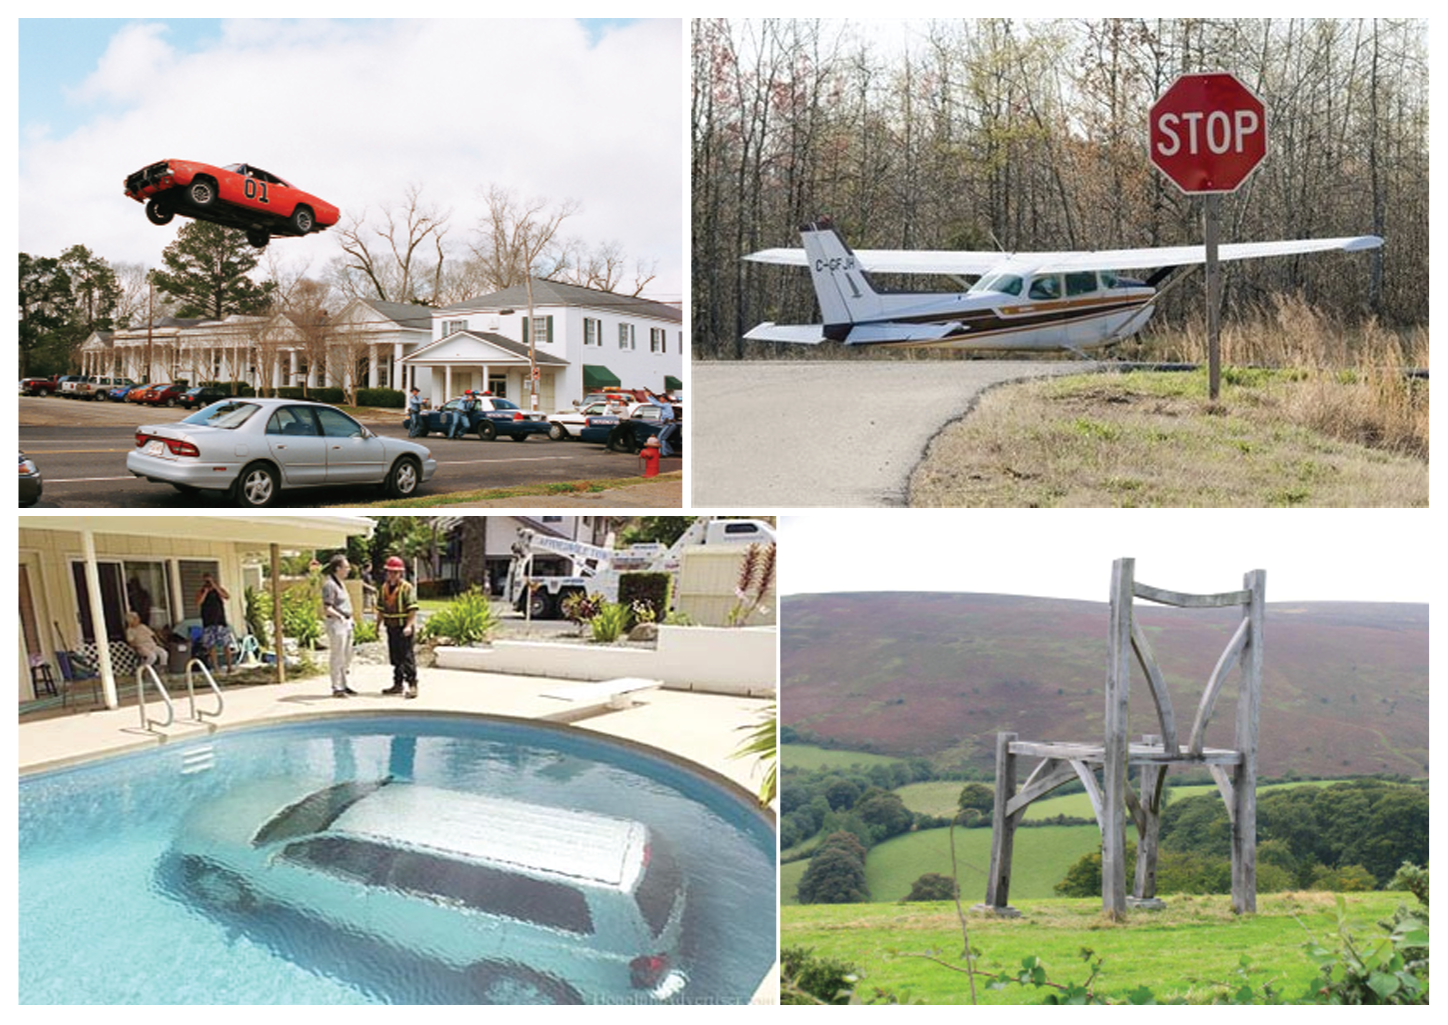
\includegraphics[width=0.5\linewidth]{figures/out_of_context_image.png}
        \caption{Sample images from \cite{Choi2012ContextMA} showing atypical scenarios involving violations of support, position, probability, size }
        \label{outcontext}
\end{figure}
    
\section{Context-driven multi-modal understanding}
\begin{figure}[h!]
    \centering
        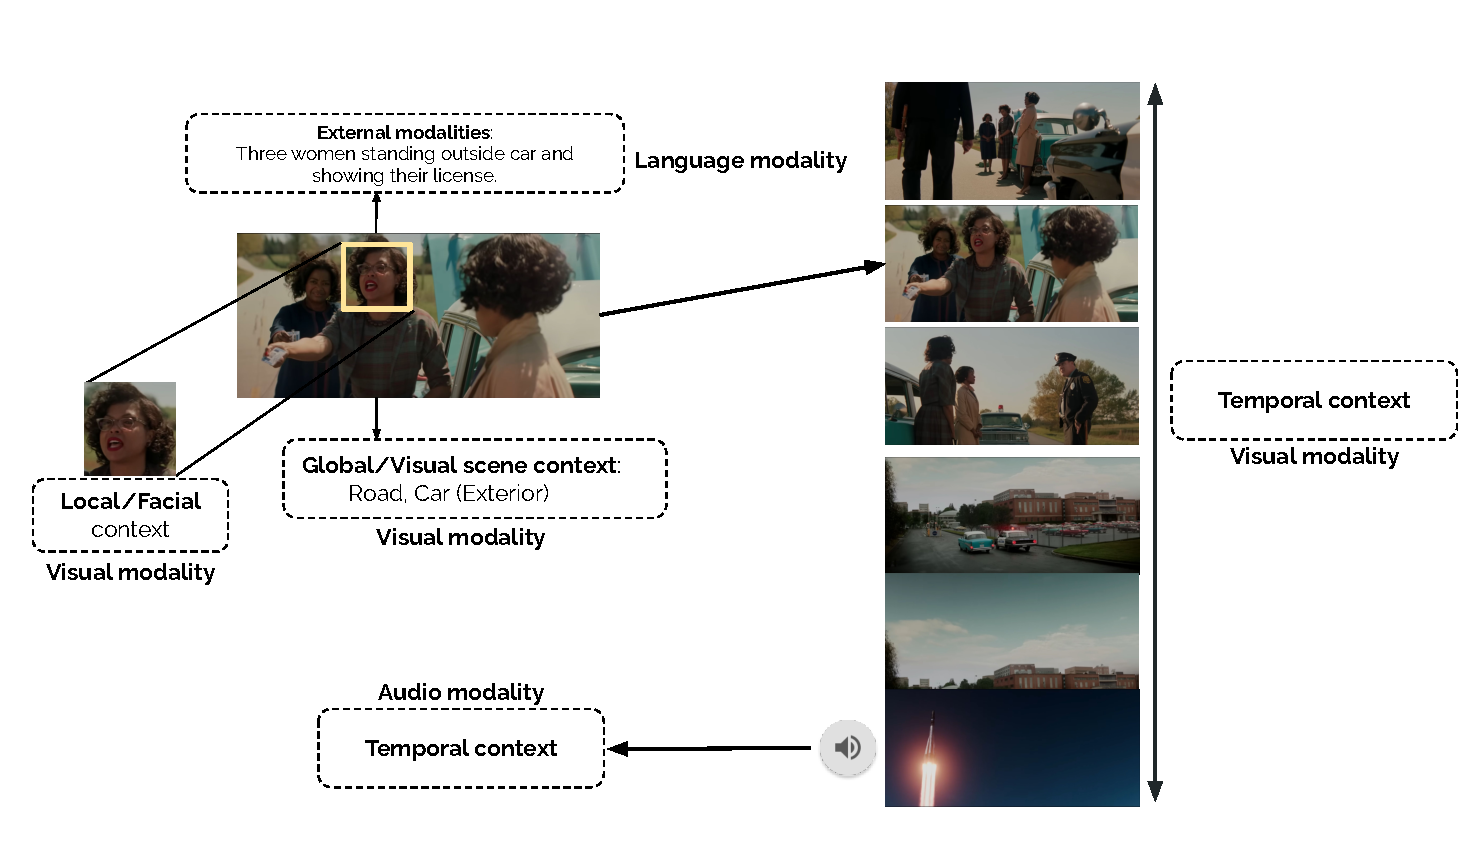
\includegraphics[width=0.9\linewidth]{figures/context_diagram.pdf}
        \caption{Outline diagram showing the presence of various contexts and associated modalities in a sample movie clip.} 
        \label{contextmultimodal}
\end{figure}
Multi-modal tasks require the processing of diverse contextual information followed by fusion for both macro and instance-level content understanding. In the case of multi-modal content, the contextual information is usually obtained through multiple input modalities. In \textbf{Fig \ref{contextmultimodal}} \footnote{Hidden Figures (2016): https://www.youtube.com/watch?v=W1VZ1-ZdQ7k\&ab\_channel=20thCenturyStudios}, we can see that the face crop of the person captures the \textbf{local/facial} context in the frame of interest. The \textbf{global} context is captured by visual scene i.e., \textbf{road, car (exterior)}. External modalities in the form of natural language descriptions, i.e., \textit{Three women standing outside the car and showing their license} provide information about the interactions happening in the foreground. Further, this frame is a part of a longer narrative, as shown in the sequence of frames. The frame sequence captures both short-term and long-term \textbf{temporal context}, where short-term context centers around local activities, including interactions between the woman and the policeman, followed by long-term temporal context involving multiple transitions within the narrative. By taking long-term temporal context into account, it can be seen that the clip ends with a spacecraft launch. Further, the sound event associated with spacecraft launch captures additional short-term temporal context.
\section{Multimodal content understanding - scale}
This work considers multimodal content understanding at two distinct scales: \textbf{instance-level} and \textbf{macro-level}. 
\subsection{Macro-level content understanding}
Macro level provides an expanded view by referring to the broad thematic elements associated with multimodal content like \textit{broad theme/topic}, \textit{underlying genre}, \textit{sentiment}, etc. As seen in Fig \ref{macro_scale_understanding} (a), the broad theme/topic, i.e., \textbf{Performing arts}, provides the macro-level view of the video. Further in Fig  \ref{macro_scale_understanding} (b), the genre, i.e., \textbf{animation}, \textbf{action}, \textbf{adventure} gives a high-level insight into the movie snippet. In our work, we consider macro-level understanding along the lines of genre for movie trailers and broad thematic elements for advertisement videos. 
\begin{figure}
 \centering
    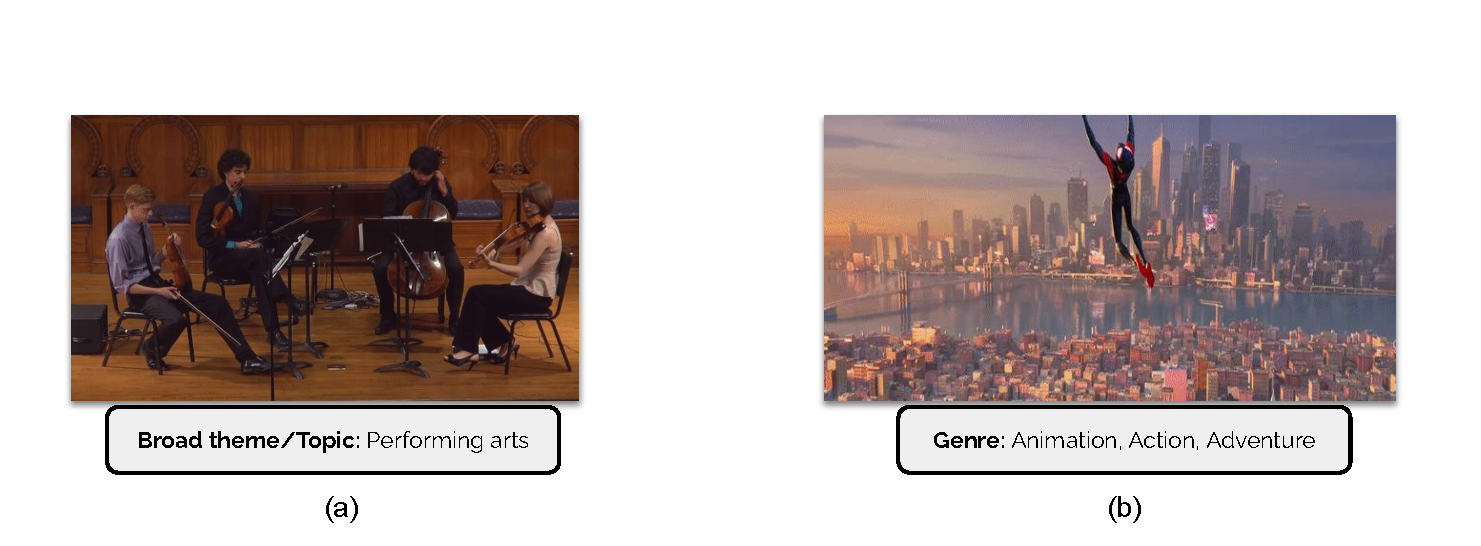
\includegraphics[width=\textwidth]{figures/macro_scale_understanding.pdf}
    \caption{Macro-level understanding examples (a) \textbf{Broad theme/topic:} Performing arts (b) \textbf{Genre:} Animation/action/adventure}
    \label{macro_scale_understanding}
\end{figure}
\subsection{Instance-level content understanding}
Instance level refers to content understanding at the scale of individual entities like objects and persons w.r.t. different attributes like \textbf{appearance}, \textbf{perceived emotional state}, \textbf{gender}, \textbf{age}, \textbf{skintone} and \textbf{occupation}. For example, in Fig \ref{instance_scale_understanding} (a) and (b), the instance-level view refers to the person with the green bounding box and the associated attributes of perceived age, gender, and affective state. In our work, we look at instance-level content understanding in terms of estimating the person's affective state.
\begin{figure}
 \centering
    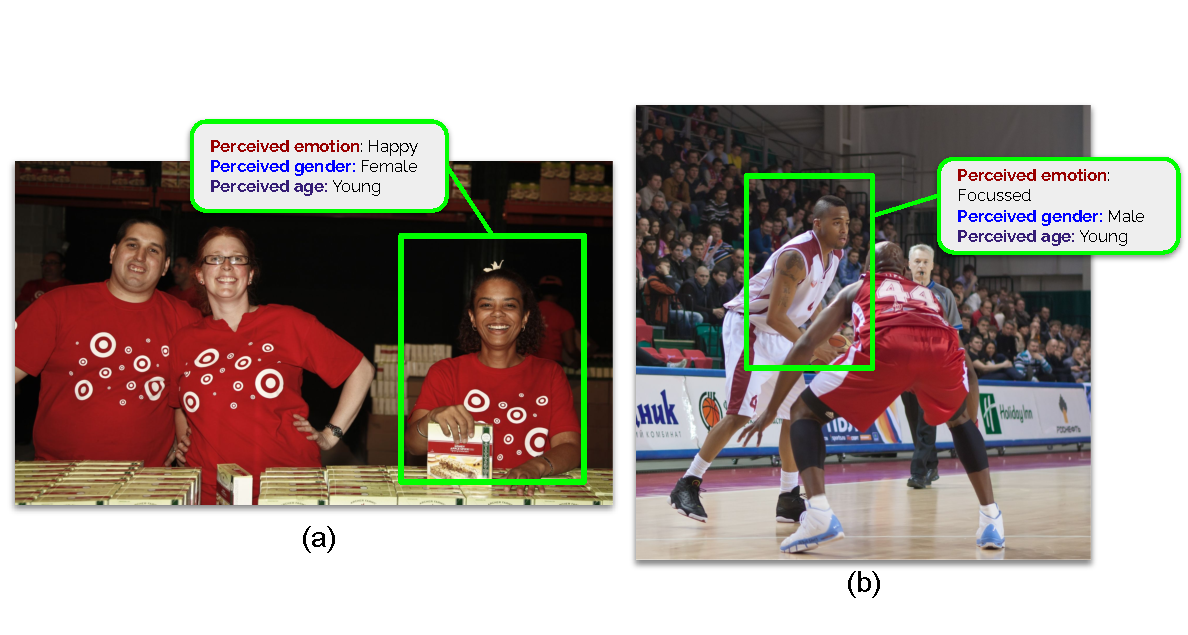
\includegraphics[width=\textwidth]{figures/instance_level_scale_understanding.pdf}
    \caption{Instance-level understanding examples. Image source: \cite{Gustafson2023FACETFI}}
    \label{instance_scale_understanding}
\end{figure}
\section{Organization and contributions}
In this section, we provide the basic outline of the thesis proposal. The proposed thesis statement is given as follows:
\begin{tcolorbox}[width=\textwidth]
Context-guided attention improves multi-modal content understanding at diverse scales.
\end{tcolorbox}
We develop contextual approaches for improved multimodal content understanding at different scales: \textbf{instance-level} and \textbf{macro-level}.  In terms of input sources, we consider multi-modal media content, including \textbf{movies}, \textbf{TV shows}, \textbf{advertisements}, and \textbf{natural scene images}. Looking at the multimodal content from both instance and macro-level viewpoints provides a holistic understanding of given inputs. In terms of the distinction between context and modalities, we use modalities available in input sources to extract diverse forms of contextual information. Further, dissimilar modalities can provide similar types of contextual information. Certain examples of contextual information obtained through multiple modalities are as follows: 

\begin{itemize}
    \item  \textbf{Visual modality:} Captures \textbf{\textit{spatial/temporal}} context through visual semantic units, i.e., objects and persons captured over images and videos.
    \item  \textbf{Language modality:} Captures \textbf{\textit{spatial (semantic)/foreground}} context through foreground based natural language descriptions of images.
    \item  \textbf{Audio modality:} Captures \textbf{\textit{temporal}} context through audio events, background music and speech.
\end{itemize}

\begin{figure}[h!]
    \centering
        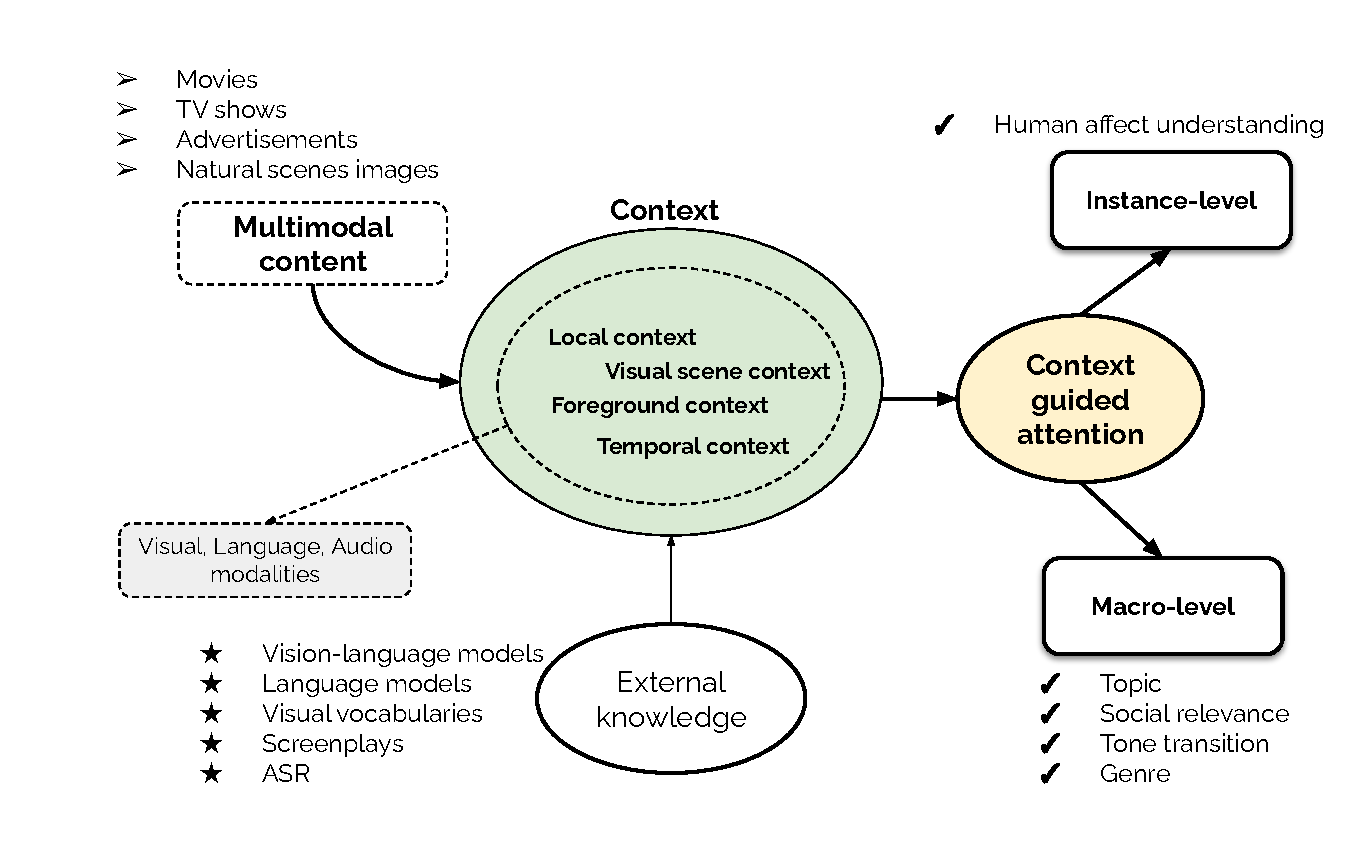
\includegraphics[width=\textwidth]{figures/Overview_diagram.pdf}
        \caption{Organization of the thesis proposal with different components}
        \label{proposalorganization}
\end{figure}

For example, both visual and audio modalities provide the necessary temporal context for various content-understanding tasks.
\par 
In the case of context processing, we leverage external knowledge from pretrained sources like vision-language models, language models, automatic speech recognition models, and domain-specific sources like screenplays and visual vocabularies. 
An outline of the proposal is shown in Fig \ref{proposalorganization}, showing the relationships between input multimodal content and content understanding at different scales. For processing the contextual information, we propose context-guided attention mechanisms to improve multimodal content understanding at two scales: macro-level and instance-level. We consider multi-modal media content, including \textbf{movies}, \textbf{TV shows}, \textbf{advertisements}, and \textbf{in-the-wild} videos as the primary input sources for exploration.
We combine the above-mentioned inputs in a content understanding framework in the following sequence of chapters:

\begin{enumerate}
    \item \textbf{Chapter 2}: We explore the problem of visual scene context processing in multi-modal data esp., movies, by leveraging external knowledge from pretrained multimodal model, i.e., CLIP \cite{Radford2021LearningTV} and domain-specific sources like screenplays, visual vocabularies. Further, we show the utility of visual scene context in improving macro-level content understanding in terms of genre.
    
    \item \textbf{Chapter 3}: We utilize our insights from Chapter 2 to propose a multimodal context fusion approach based on attention mechanism for human affect (\textbf{instance-level}) understanding in natural scenes and TV shows.
    
    \item \textbf{Chapter 4}: We explore the fusion of foreground and temporal context through multiple input modalities for macro-level understanding in advertisement videos along the lines of topic, tone transitions, and social relevance. 
    
    \item \textbf{Chapter 5}: We propose an efficient information-theoretic framework to fuse contextual information in multimodal pretrained transformers for content understanding tasks across different scales.
\end{enumerate}

\textbf{Chapter 5} is an ongoing work and will be extended into post-proposal for integration into the final thesis dissertation.


% Research Topic 1
\chapter{Visual scene context recognition through multimodal guidance}

In this chapter, we consider the task of recognizing visual scene context in media content by leveraging pre-trained multimodal information.  
\section{Role of scene as contextual signal}
Visual scene context refers to the global context in the image, including the relationship of the target objects with the environment/location and other co-occurring objects \cite{Bar2004VisualOI}, \cite{Qiao2021ObjectLevelSC}. Visual scene context drives the likelihood of finding particular objects spatially co-located with each other. For example, as shown in Fig \ref{station_kitchen}, utensils are more likely to be present in the kitchen as compared to the train station. 
Apart from the domain of natural scenes, understanding the visual scene context is also important in the case of media content \cite{CMI} esp. movies and curated short content like advertisements. 
\par
In cinematic terms, \textit{mis-en-scene} \cite{Bordwell1979FilmAA} refers to how the different elements of a film are depicted and arranged in front of camera. Key components of \textit{mis-en-scene} include the actors with their different styles, \textbf{visual scenes} where the interactions take place, set design including lighting and camera placement, and the accompanying costumes and makeup of the artists. The visual scene is considered a crucial component since it sets the mood and provides a background for the various actions performed by the actors in the scene. Visual scenes in movies are often tied to social settings like weddings, birthday parties, and workplace gatherings that provide information about character interactions. Accurate recognition of visual scenes can help in uncovering the bias involved in the portrayal of under-represented characters vis-a-vis different scenes, e.g., fewer women shown in the office as compared to the kitchen. For content tagging tasks like genre classification, visual scenes provide context information like battlefield portrayals in action/adventure movies, space-shuttle in sci-fi movies, or courtrooms in dramas.
\par 
In the following section, we highlight certain challenges associated with visual scene recognition, especially w.r.t. movies.
\begin{figure}[h!]
    \centering 
     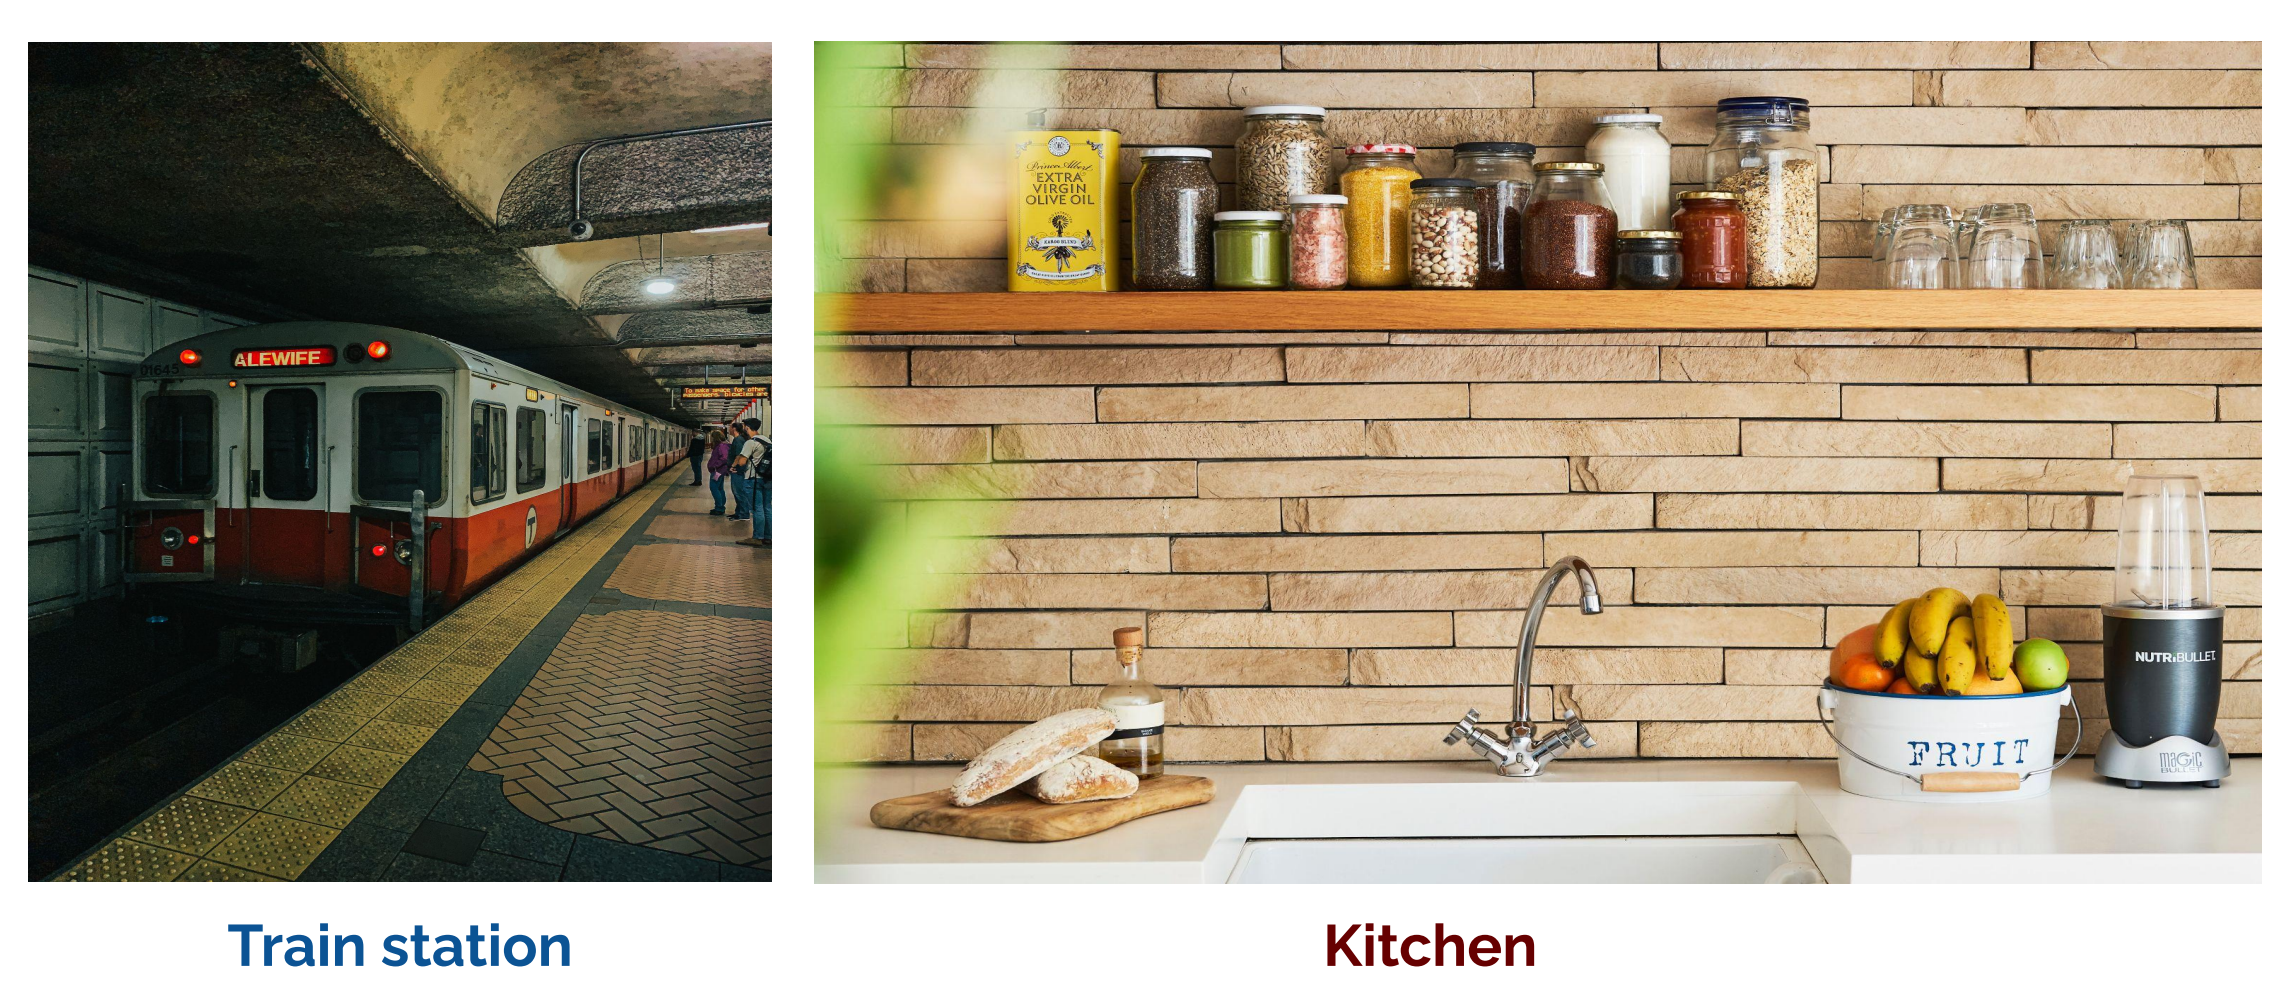
\includegraphics[width=0.6\linewidth]{figures/train_station_kitchen.png}
     \caption{Difference between visual scenes - train station and kitchen in terms of object placements.}
     \label{station_kitchen}
\end{figure}
% Use reference: \textit{Structure Inference Net: Object Detection Using Scene-Level Context and Instance-Level Relationships} here.
\section{Movies vs Natural scenes}
Visual scene recognition, in the case of static images, is primarily driven by natural scenes due to large-scale datasets like SUN397 \cite{Xiao2010SUNDL} and Places-2\cite{zhou2017places}. However, there are certain inherent challenges in visual scene recognition for movies that need to be addressed, as shown in Fig \ref{Intro figure}.
\begin{figure}[!h]
 \centering
  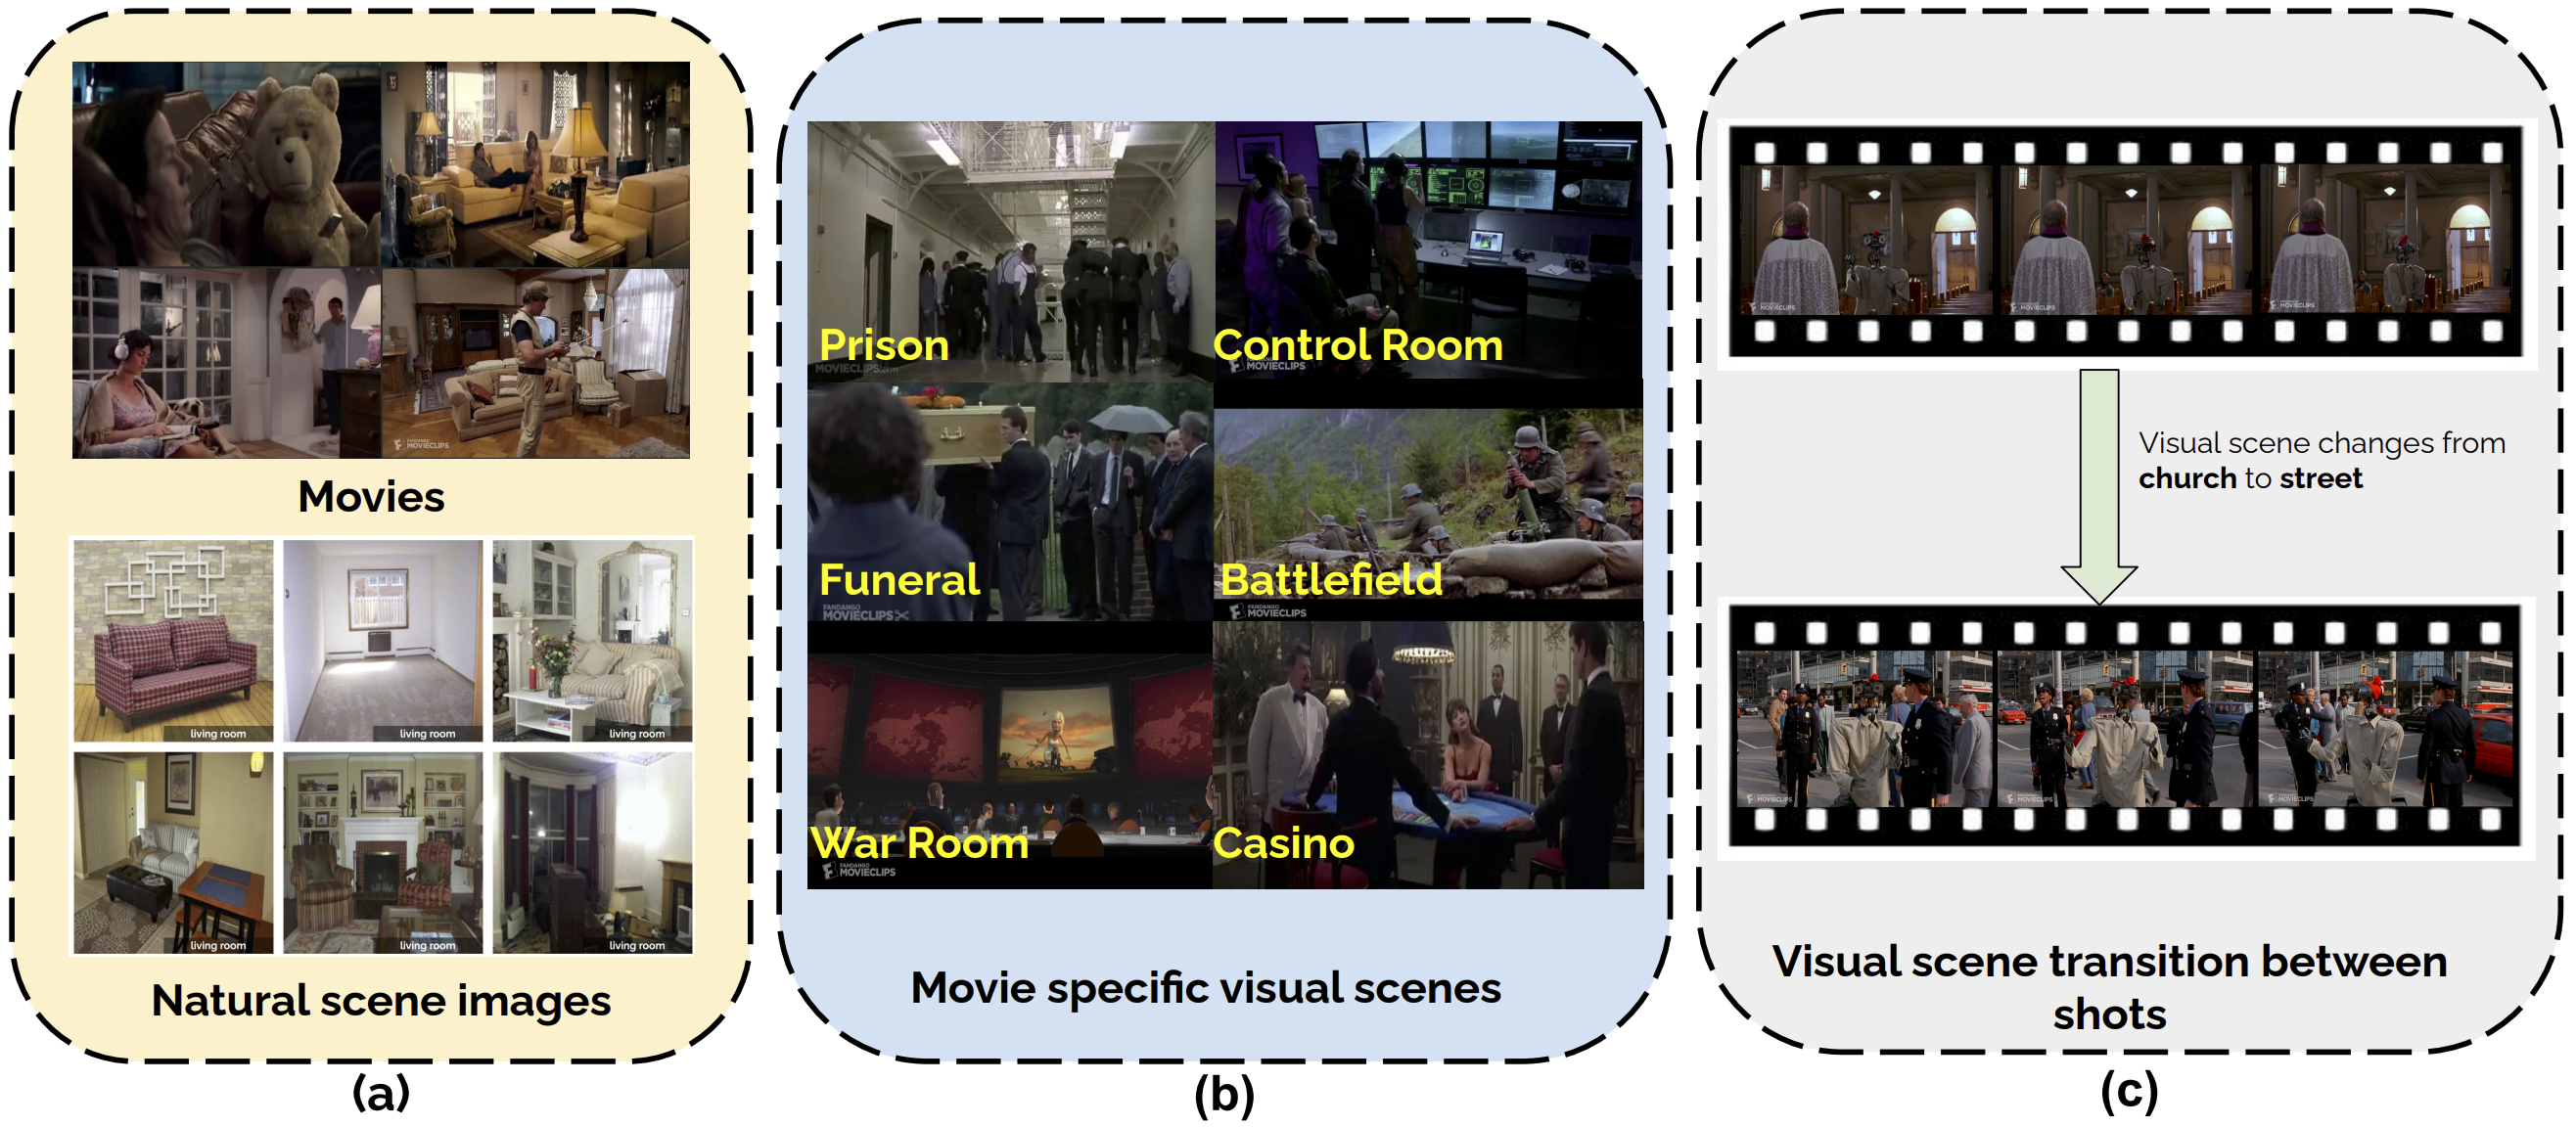
\includegraphics[width=0.8\linewidth]{figures/Introduction_Figure.png}
  \caption{Overview diagram highlighting the challenges associated with visual scene recognition in movies (a) Domain mismatch between Natural scene images,(Source: \url{http://places2.csail.mit.edu/explore.html}) vs frames from Movies for \textbf{living room} (b) Movie centric visual scene classes like prison, control room etc that are absent from existing taxonomies (c) Change in visual scene between shots in the same movie clip.}
  \label{Intro figure}
\end{figure}
\textbf{\underline{Domain mismatch - scene images vs. movie frames:}} Visual scenes depicted in movies are distinct compared to natural scenes due to increased focus on actors, multiple activities, and viewpoint variations like extreme closeup, wide-angle shots etc. An example is shown in Fig.~\ref{Intro figure} (a) for images from Places2 dataset \cite{zhou2017places} and movie frames from Condensed Movies dataset \cite{bain2020condensed}.\\
\textbf{\underline{Lack of completeness in scene taxonomy:}} Movies depict both real-life and fictional scenarios that span a wide variety of visual scenes. As shown in Fig.~\ref{Intro figure}(b), certain movie-centric visual scene classes like \textit{battlefield}, \textit{control room}, \textit{prison}, \textit{war room}, \textit{funeral}, \textit{casino} are absent from existing public scene taxonomies associated with natural scene image and video datasets.\\
\textbf{\underline{Lack of shot-specific visual scene annotations:}} Existing datasets like Condensed Movies \cite{bain2020condensed} and VidSitu \cite{Sadhu_2021_CVPR} provide a {\em single} visual scene label for the entire movie clip (around 2 minutes long), obtained through descriptions provided as part of YouTube channel Fandango Movie clips \footnote{https://www.youtube.com/channel/UC3gNmTGu-TTbFPpfSs5kNkg}. In Fig.~\ref{Intro figure} (c), the provided description: \textit{Johnny Five (Tim Blaney) searches for his humanity in the \textbf{streets} of New York.} mentions only the visual scene \textbf{street}, while the initial set of events takes place inside \textbf{church}. Instead of considering a single scene label for the entire movie clip, shot-level visual scene annotation can help in tracking the scene change from \textbf{church} to \textbf{street}.
\section{Contributions}
In our work, we consider shots within a given movie clip as the fundamental units for visual scene analysis since shots consist of consecutive set of frames related to the same content, whose starting and ending points are triggered by recording using a single camera \cite{SBD}. Our contributions are as follows:
Our contributions are as follows:
\begin{itemize}
\item \textbf{Language guided Movie-centric scene taxonomy:} We develop a movie-centric scene taxonomy by leveraging scene headers (sluglines) from movie scripts (language-based sources) and existing video datasets with scene labels like HVU\cite{diba_large_2020}. 
\item \textbf{Automatic shot tagging:} We utilize our generated scene taxonomy to automatically tag around 1.12M shots from 32K movie clips using a pretrained vision-language model called CLIP \cite{CLIP} based on a frame-wise aggregation scheme.  
\item \textbf{Multi-label scene classification:} We develop multi-label scene classification baselines using the shot-level tagged dataset called MovieCLIP and evaluate them on an independent shot-level dataset curated by human experts. 
\item \textbf{Downstream tasks:} We further extract feature representations from the baseline models pretrained on MovieCLIP and explore their applicability in diverse downstream tasks of multi-label scene and movie genre classification from web videos \cite{diba_large_2020} and trailers \cite{2019Moviescope}, respectively. 
\end{itemize}
\section{Related work}
\textbf{Image datasets for visual scene recognition:}
Image datasets for scene classification like MIT Indoor67 \cite{IndoorScenes} relied on categorizing a finite set of (67) indoor scene classes. A broad categorization into indoor, outdoor (natural) and outdoor (man-made) groups for 130K images across 397 subcategories was introduced by the SUN dataset \cite{xiao_sun_2016}. For large-scale scene recognition, the Places dataset \cite{zhou2017places} was developed with 434 scene labels spanning 10 million images. The scene taxonomy considered in the Places dataset was derived from the SUN dataset, followed by the careful merging of similar pairs. It should be noted that the curation of large-scale visual scene datasets like Places relied on crowd-sourced manual annotations over multiple rounds.\\
\section{Role of multi-modality:}
    \subsection{Language driven taxonomy curation}
    \subsection{Usage of vision-language models}
    \subsubsection{CLIP: Learning Transferable Visual Models From Natural Language Supervision}
    \subsection{MovieCLIP dataset}
    \subsubsection{CLIP-based visual tagging}
    \subsubsection{Analysis of CLIP tagging}
    \subsubsection{Quality estimation through human verification}
\section{Experiments and Results:}
\subsection{Experimental Setup}
\subsection{Visual scene recognition - Movies}
\subsection{Downstream tasks}
\subsubsection{Visual scene recognition - web videos}
\subsubsection{Multi label genre classification - movie trailers}
\subsubsection{Impact of MovieCLIP pretraining}
\section{Ethical implications}
\section{Conclusion}

\chapter{Human affect understanding through multimodal context driven fusion}
In the previous chapter, we explored how visual scene context information can be extracted from multimodal sources, especially media content, by utilizing large-scale pretrained external multimodal models. In this chapter, we will investigate the usage of contextual signals for instance-level multimodal content understanding. We consider instance-level multimodal content understanding along the granularity of individual persons and their perceived affective states in the scene. 
\section{Human affect understanding}
 There has been increased interest in understanding the affective processes associated with various facets of human emotions \cite{dukes2021}. An integral part of affective understanding is the ability to infer expressions of human emotions from various sources like images \cite{AICA}, speech \cite{speechemo}, and language use \cite{Poria2019EmotionRI}, as seen in Fig \ref{}. Affect recognition systems have enabled multiple human-centered applications, notably in healthcare (depression detection \cite{depressiondetection}, autism-spectrum diagnosis \cite{autismguha}) and learning \cite{savchecnkoengagement}).

\begin{figure}[h!]
    \centering
    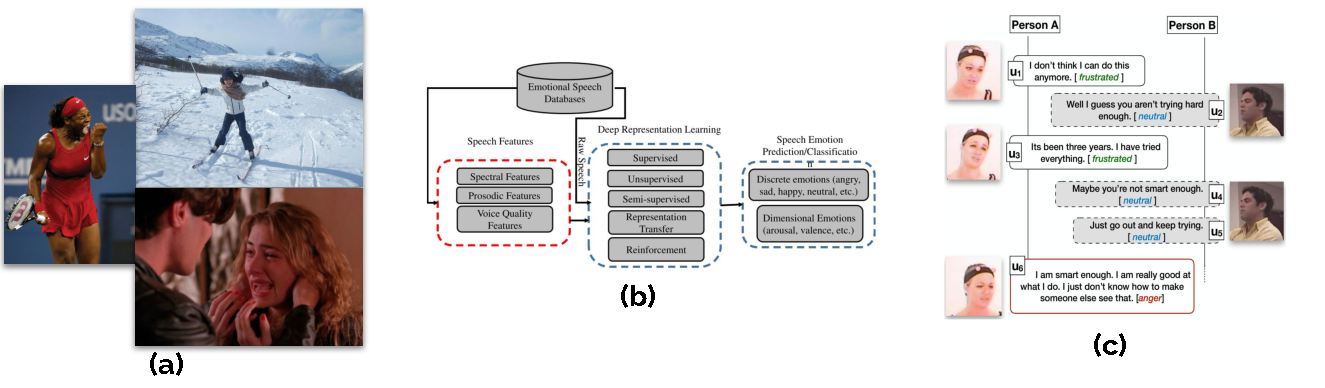
\includegraphics[width=\textwidth]{figures/emotion_overview.pdf}
    \caption{Overview of sources associated with different modalities (mentioned in brackets). \textbf{(a)} images (\textbf{visual}) \textbf{(b)} speech (\textbf{audio}) \textbf{(c)} language (\textbf{language}).}
    \label{emotion overview}
\end{figure}

 
\subsection{Facial expression - Is it the complete picture?}

Affect recognition from images has primarily focused on facial expressions \cite{DFEW,Mollahosseini2019AffectNetAD} along a fixed set of categories. Moreover, facial expression-based methods typically consider crops of a single face, which might provide ambiguous signals for classifying perceived emotions. An example where the face crop doesn't provide a complete picture for decoding the human affective state is shown in Fig \ref{face crop}. In Fig \ref{face crop} (a), we can see that the face crop for the child indicates a perceived affective state of surprise. But after including the entire global scene context, it can be inferred that the child is feeling happy and excited due to the event, i.e., birthday.
Further, in Fig \ref{face crop} (b), we can see that the face crop provides a noisy and incomplete picture. After taking into account the surrounding context that involves a troublesome situation of flooding, it can be assumed that the woman is feeling annoyed. Hence, in this work, we aim to include contextual cues from the visual scene and foreground interactions that contribute to the perception of affective state.

\begin{figure}[h!]
    \centering
    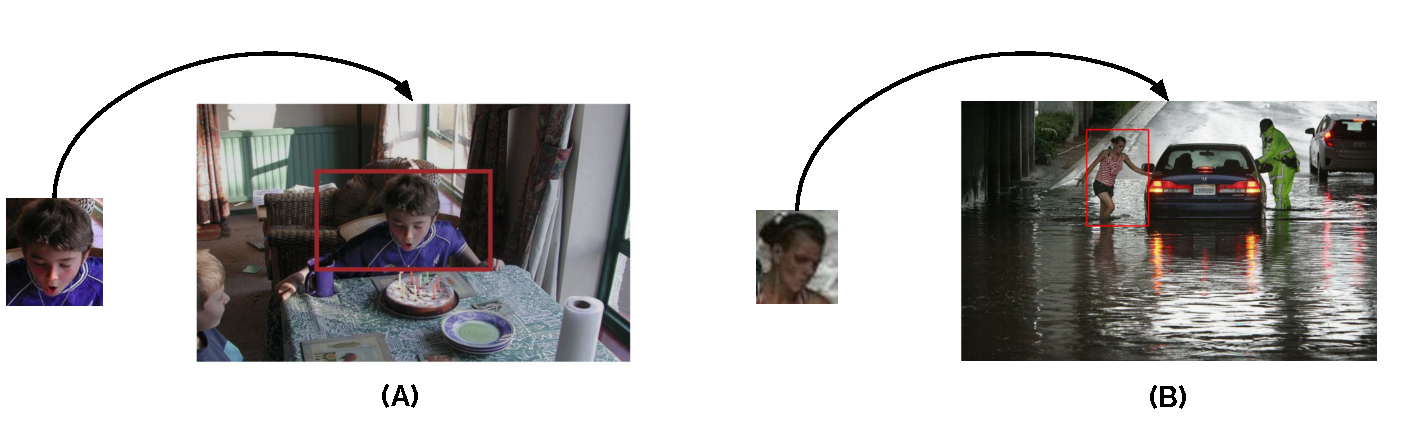
\includegraphics[width=\textwidth]{figures/face_crop_drawings.pdf}
    \caption{Examples from \textbf{EMOTIC} dataset where \textbf{(a)} face crop only provides an incomplete picture \textbf{(b)} face crop provides a noisy signal }
    \label{face crop}
\end{figure}


\section{Role of context in affect perception}
\textbf{Context in Emotion Perception:} The role of context extraneous to a person (beyond their traits and behavior) in the perception of their expressed emotion has been studied from the perspective of scenes \cite{BarretEmotionPerception}, and cultures \cite{Masuda2008PlacingTF}. In \cite{Dudzik2019ContextIH}, the perceivable-encoding context and the prior knowledge available with the perceivers are reported as the major sources of context for influencing emotion perception.  Situational context, like reactions from other people, has been considered in \cite{Wieser2012FacesIC} as a means to decode emotional states of persons in consideration.\\
\textbf{Context-based image datasets:} Image-based emotion recognition datasets like AffectNet \cite{AffectNet}, FER \cite{BarsoumICMI2016}, DFEW \cite{DFEW} primarily focus on signals encoded in facial expressions. Since emotion perception depends on where the facial configuration is present, datasets like EMOTIC \cite{kostiPAMI} and CAER \cite{CAER-S} have been proposed to incorporate contextual information in terms of visual scenes and social interactions. In the case of EMOTIC, annotators have marked person instances in unconstrained environments with apparent emotional states based on the existing scene context. However, the annotation process in CAER revolves around TV shows with primary focus on interactions-driven context. 
\\
\textbf{Context modeling approaches:} 
\cite{kostiPAMI,CAER-S} explore context modeling in terms of dual stream models for processing body and whole image streams. \cite{CAGER} also uses a dual stream network with context stream, modeled using an affective graph composed of region proposals.\cite{Mittal2020EmotiConCM} uses depth and pose as additional contextual signals with existing streams like scene, face for predicting person-specific emotion.
\cite{pikoulis2021leveraging} explores contextual modeling in short movie clips by considering scene and action characteristics along with body (including face) based signals. In contrast, our approach uses natural language descriptions to describe the foreground context along with scene and person-specific streams.
\\
\textbf{Multimodal vision-language models:} Vision language (VLN) models like OFA \cite{wang2022ofa}, VL-T5 \cite{cho2021vlt5}, ALBEF \cite{ALBEF} are pretrained on large-scale image-text pairs curated from the web, thus enabling its usage in diverse tasks like image captioning, retrieval, visual-question answering etc. In our formulation, we harness the capabilities of VLN models to generate descriptive captions since they contain condensed descriptions of the foreground context in terms of entities, including persons.


\section{Human affect understanding framework}

\begin{figure}[h!]
    \centering
    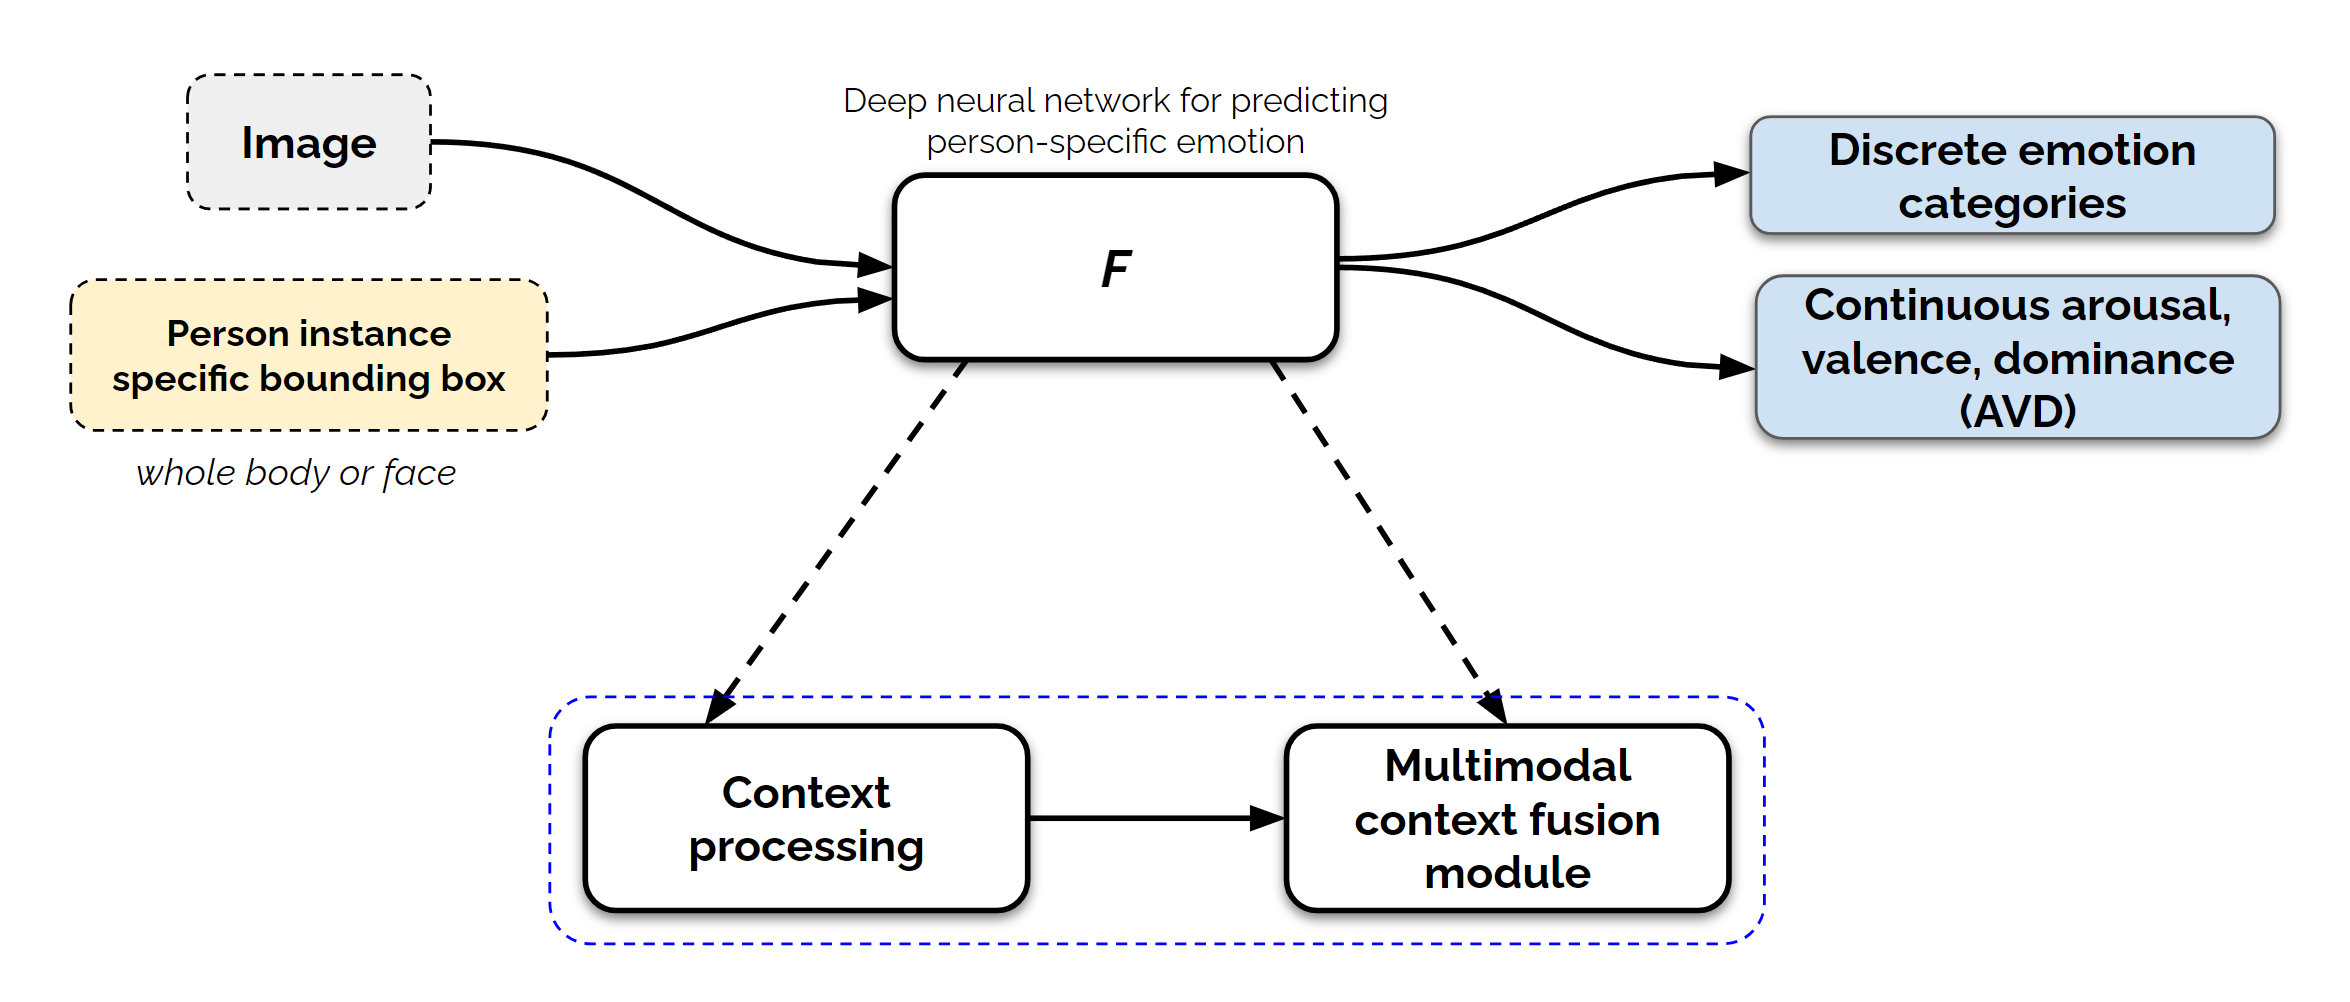
\includegraphics[width=\textwidth]{figures/human_affect_understanding.png}
    \caption{Outline of the human affect understanding framework }
    \label{human affect understanding}
\end{figure}

As seen in fig \ref{human affect understanding}, the human affect understanding relies on a neural network-based framework \textbf{\textit{F}} that consists of two segments: \textbf{Context processing} and \textbf{Multimodal context fusion module}. In terms of formal definition, given an image $I$ and a person-specific context in the form of bounding box $[x,y,w,h]$, the task is to predict the emotional state $p$ associated with a person as $p_{disc}, p_{cont} = F(I,[x,y,w,h])$. $p_{disc}$ and $p_{cont}$ refer to the predicted set of discrete emotion categories and continuous arousal, valence, and dominance values, respectively.

\section{Contextual processing - Multimodality:}

We extract contextual information through multiple modalities and use them for our subsequent instance-level content understanding task, i.e., affect estimation of a person. The outline of the context processing through different modalities is shown in Fig \ref{context_extraction}.

\begin{figure}
    \centering
    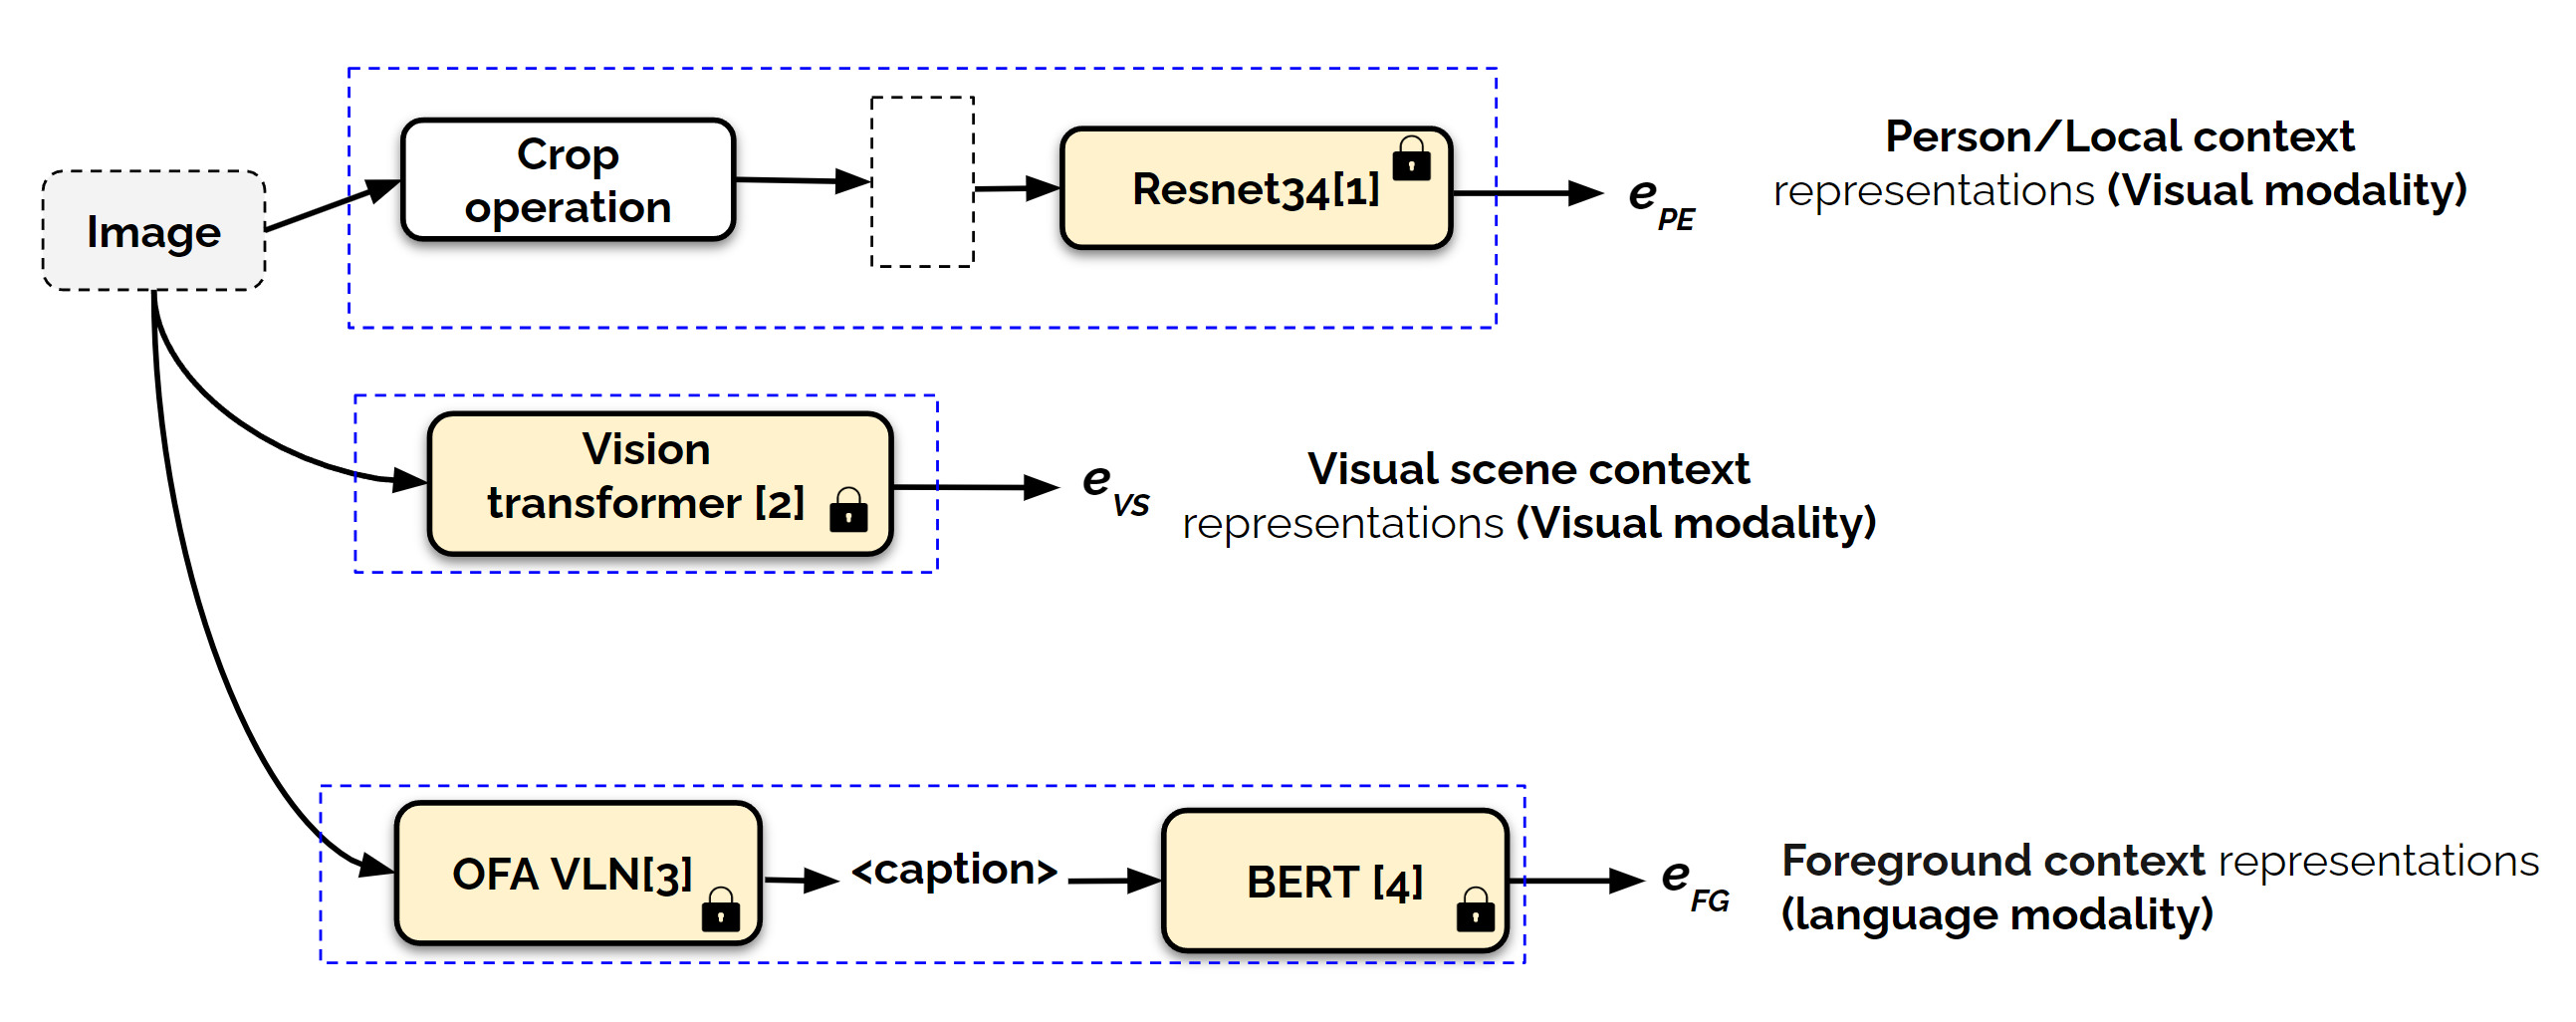
\includegraphics[width=\textwidth]{figures/context_extraction_multimodality.png}
    \caption{Outline of context processing through various modalities}
    \label{context_extraction}
\end{figure}
In the following subsections, we outline the process associated with the extraction of context information from the image.

\subsection{Visual scene context}
The underlying visual scene ($VS$) (e.g.,  kitchen, bar, football field etc) plays a role in influencing the emotional state of a person. Here we use a ViT \cite{Dosovitskiy2021AnII} model ($f_{VS}$) finetuned on Places365 \cite{zhou2017places} as the backbone network for extracting visual scene representations ($e_{VS}$) from $I$.
\subsection{Person-specific context}
The person-specific context is extracted using a whole-body or facial bounding box, denoted by $[x,y,w,h]$ from image $I$. The cropped person instance is passed through a person encoder ($f_{PE}$), i.e., Resnet34~\cite{He2016DeepRL} for extracting person-centric representations ($e_{PE}$). 
\subsection{Language-driven foreground context}
 Natural language description of image $I$ provides foreground (FG) context in terms of entities, including persons and their interactions. We use a 12-layer transformer encoder-decoder model $OFA_{large}$ \cite{wang2022ofa} as $f_{expert}$ to extract the foreground-specific captions for image $I$. For extracting text representations ($e_{FG}$) of the captions, we use BERT's \cite{Devlin2019BERT} pretrained encoder ($f_{FG}$) from HuggingFace \cite{wolf-etal-2020-transformers}.
\section{Multimodal context fusion module}

We propose a multimodal context fusion module to process the interaction of the person instance with foreground and background (visual scene).
\begin{figure}[h!]
    \centering
    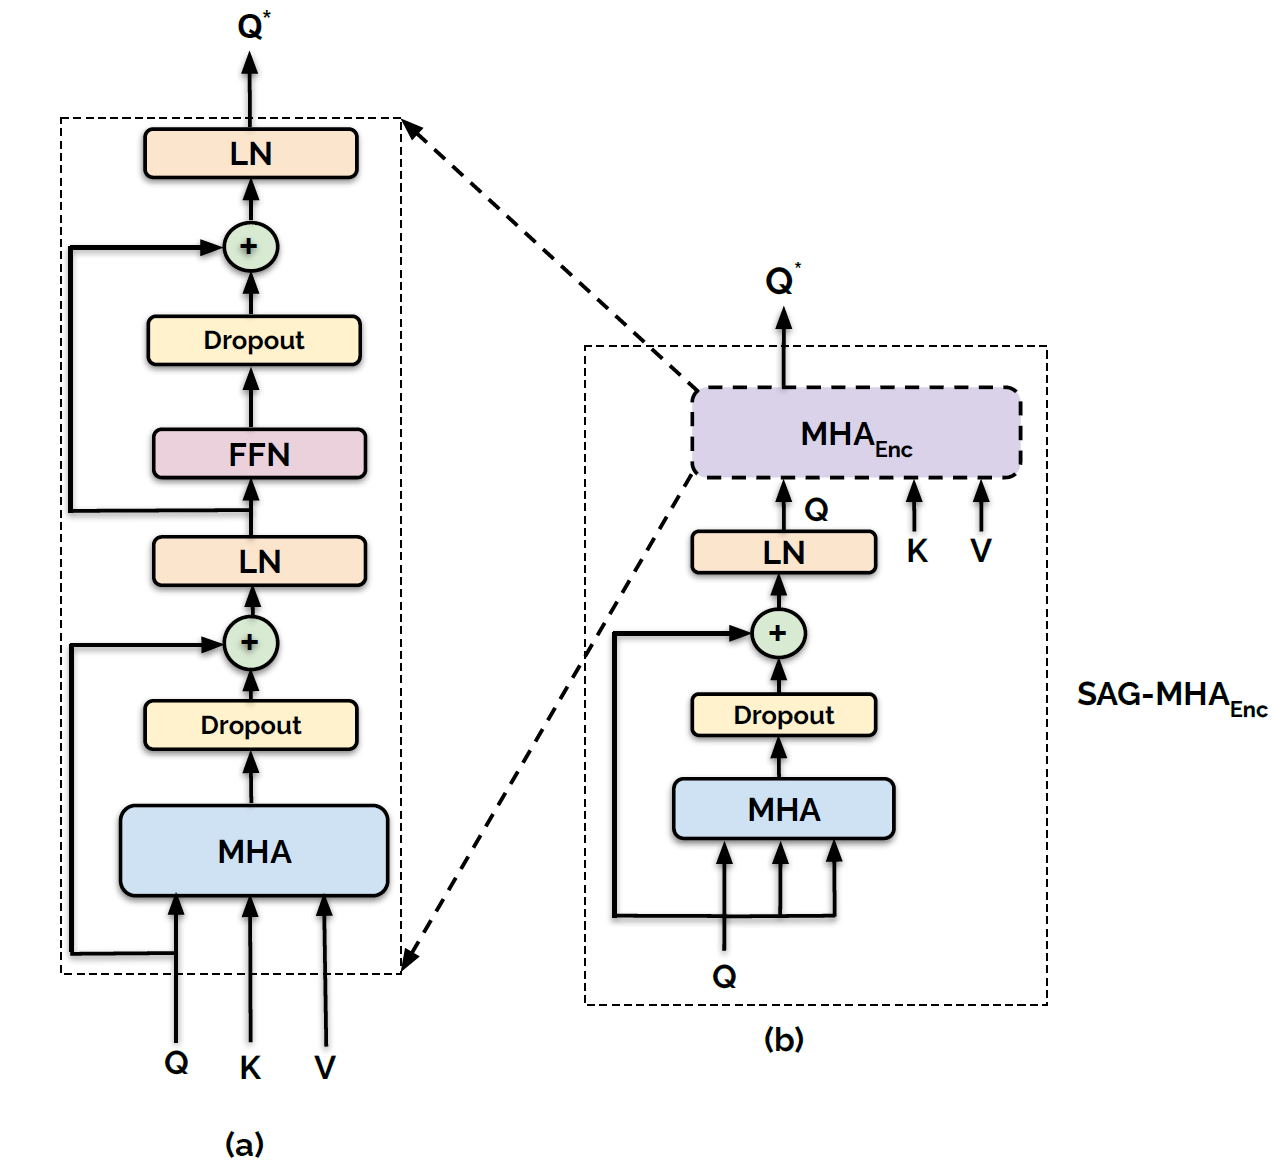
\includegraphics[width=0.7\textwidth]{figures/SAG_MHA.png}
    \caption{Outline of (a) MHA\textsubscript{enc} (b) SAG-MHA\textsubscript{enc} layers. \textbf{LN}: Layer Norm, \textbf{FFN}: Feedforward network, \textbf{MHA:} Multihead attention, \textbf{SAG:} Self Attention Augmented}
    \label{encoder block}
\end{figure}
The multimodal context fusion module is composed of two parallel streams, associated with foreground and visual scene-based contexts. The basic operation in individual streams is a cross-modal encoder block CM\textsubscript{enc} composed of L encoder layers. As shown in Fig \ref{encoder block}, we consider two designs for the encoder layer i.e., MHA\textsubscript{enc} and SAG-MHA\textsubscript{enc}.  
The set of operations in encoder MHA\textsubscript{enc} layer for query ($Q$), key ($K$) and value ($V$) representations are listed as follows:
\begin{equation} \label{MHAEnc operation}
\begin{split}
 Q^{'} & = LN(Q + \text{Dropout}(MHA(Q,K,V))) \\ 
Q^{*} & =LN(\text{Dropout}(FFN(Q^{'}))+Q^{'})
\end{split}
\end{equation}
Here $MHA$, $LN$ and $FFN$ refer to Multi-head attention, layer-norm operation and feed-forward neural network respectively. The SAG-MHA\textsubscript{enc} layer consists of a multi-head attention based transformation of the query representations followed by input to the MHA\textsubscript{enc} layer. The design of SAG-MHA\textsubscript{enc} is inspired from multimodal co-attention layer proposed in \cite{yu2019mcan} for visual question answering task.
\begin{equation} \label{SAG-MHAEnc operation}
\begin{split}
 Q^{'} & = LN(Q + \text{Dropout}(MHA(Q,Q,Q))) \\ 
Q^{*} & = MHA_{enc}( Q^{'},K,V) 
\end{split}
\end{equation}
In CM\textsubscript{enc}, the output from the $i$th encoder layer $Enc_{i}$ is passed as query ($Q$) to the subsequent layer with the key ($K$) and value ($V$) remaining the same. Here, $Enc_{i}$ layer can be either MHA\textsubscript{enc} or SAG-MHA\textsubscript{enc}.
\begin{equation} \label{encoder layer operation}
\begin{split}
    Q_{i}&=Enc_{i}(Q_{i-1},K,V) \     i > 0 \\
    Q_{0} &=Enc_{0}(Q,K,V)
\end{split}
\end{equation}
We use separate CM\textsubscript{enc} blocks for processing the foreground and visual scene-guided context streams. MCF (MHA\textsubscript{enc}) and MCF (SAG-MHA\textsubscript{enc}) consists of 4 MHA\textsubscript{enc} layers (8 heads and hidden dimension=512) and 3 SAG-MHA\textsubscript{enc} layers (8 heads and hidden dimension=768) in the CM\textsubscript{enc} blocks respectively.

\begin{figure}[h!]
    \centering
    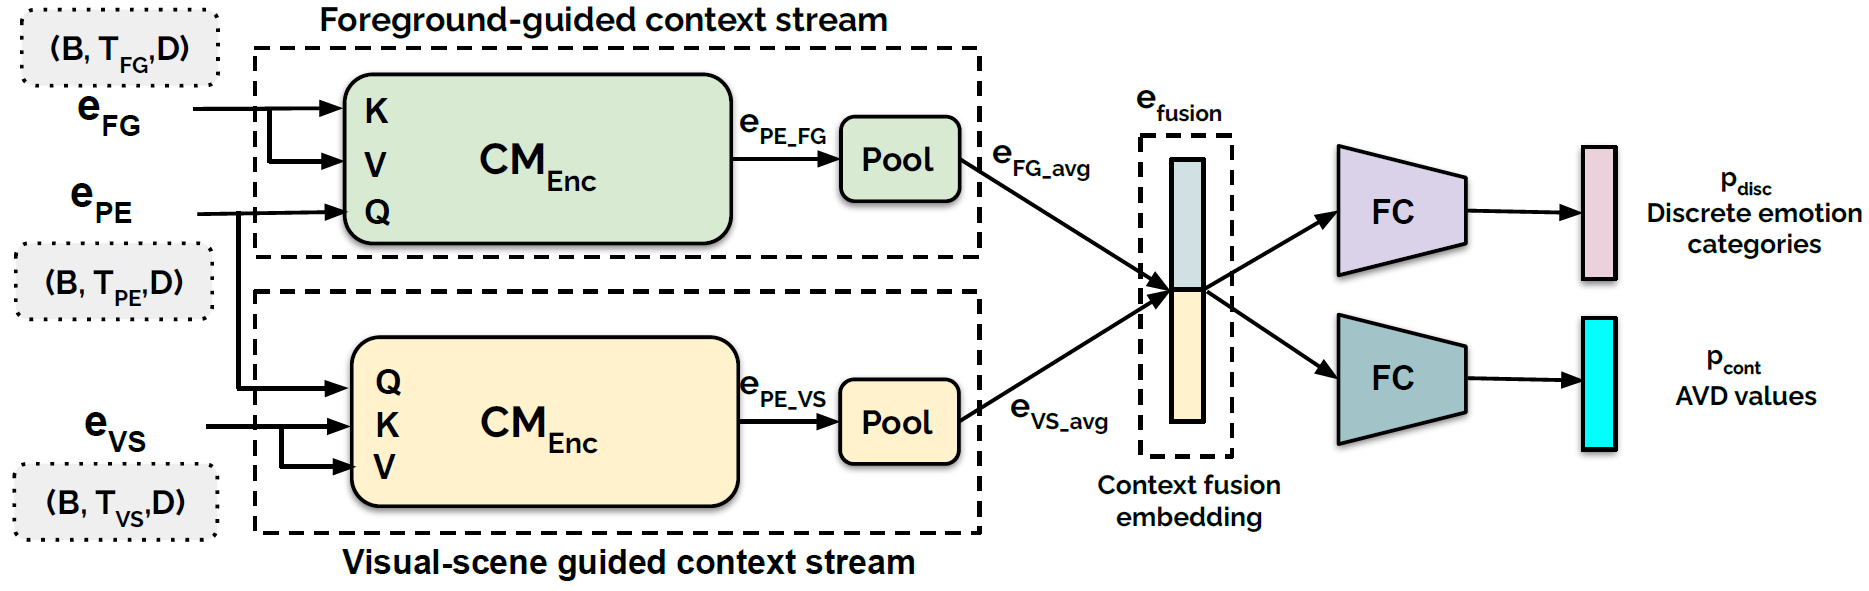
\includegraphics[width=\columnwidth]{figures/MCF_module_updated.png}
    \caption{Outline of the $MCF$ module. Separate CM\textsubscript{enc} blocks are used to model the foreground and visual scene context streams. $B$: Batch size. $D$: Hidden dimension. Token length of $T_{FG}$: text representations, $T_{PE}$: person representations, $T_{VS}$: visual scene representations. AVD: Arousal, Valence, Dominance
    }
    \label{mcf module}
\end{figure}
The details of the respective context-guided streams are listed as follows:\\
\textbf{\underline{Foreground-guided context stream:}} We use $e_{PE}$ as query ($Q$) and $e_{FG}$ as key and value inputs to the CM\textsubscript{enc} encoder.\\
\textbf{\underline{Visual-scene guided context stream:}} Similar to the foreground-guided context stream, we use $e_{PE}$ as query ($Q$) and $e_{VS}$ as key and value inputs to the CM\textsubscript{enc} encoder.\\
\textbf{\underline{Context fusion:}}
The outputs from the context-guided streams i.e., $e_{PE\_{FG}}$ and $e_{PE\_{VS}}$ are average pooled and concatenated to obtain a fused embedding as: $e_{fusion}=[e_{FG\_{avg}};e_{VS\_{avg}}]$
\section{Experiments}
\subsection{Emotic}

We use a non-intersecting split of 13584 and 4389 images for training and validation. For testing we use the publicly available split of 5108 images. For joint prediction of 26 discrete emotion classes and the continuous-valued AVD ratings, we use multiple fully-connected (FC) heads in the $MCF$ module with $e_{fusion}$ as input (Fig \ref{mcf module}). The person specific instance in each image is defined by the ground truth person box. We do not consider face as a part of person-specific context since approx 25\% of images do not have visible faces. \\
For training $MCF$ with MHA\textsubscript{enc} and SAG-MHA\textsubscript{enc} layers, we use AdamW \cite{AdamW} (\textit{lr=2e-5}) and Adam \cite{Adam} (\textit{lr=2e-4,  exp($\gamma$=0.90)}) with batch sizes 32 and 64 respectively. \footnote{exp is exponential scheduler \label{note1}}. We use SGD(\textit{lr=1e-2, exp($\gamma$=0.90)}) with a batch size of 64 while training the person-crop only Resnet34 model ($PO_{R34}$) in Table \ref{ablationemotic}. For training all the models associated with EMOTIC, we use a weighted combination of binary-cross entropy (BCE) and mean squared error (MSE) losses.
\begin{equation}
Loss =\lambda_{1} BCE(p_{disc},y_{disc}) + \lambda_{2} MSE(p_{cont},y_{cont})
\end{equation}
Here $y_{disc}$ and $y_{cont}$ refer to ground truth discrete emotion labels and continuous arousal valence dominance ratings. The optimal weights $\lambda_{1}$ and $\lambda_{2}$ are tuned using the validation split. 

\subsection{CAER-S}

We use a non-intersecting split of 39099 and 9769 video frames across 79 TV shows for training and validation. For testing, we use the public split of 20913 video frames. Since face is a dominant signal for persons in TV shows, we use MTCNN \cite{MTCNN} \footnote{https://github.com/timesler/facenet-pytorch} to obtain face crops. We have a single fully connected (FC) head with $e_{fusion}$ as input for predicting 7 discrete emotion classes. \\
For training $MCF$ with MHA\textsubscript{enc} and SAG-MHA\textsubscript{enc} layers, we use Adam (\textit{lr=2e-4, exp($\gamma$=0.90)}) with a batch size of 64. We use Adam (\textit{lr=1e-4, exp($\gamma$=0.75)}) with a batch size of 64 while training the face-crop only Resnet34 model ($FO_{R34}$) in Table \ref{ablationCAER-S}. For training all the models associated with CAER-S, we use multi-class cross-entropy loss.
\\
We conduct our experiments using the Pytorch \cite{Paszke2019PyTorchAI} library. We set the maximum sequence length $T_{FG}$ as 512 for the captions (Fig \ref{mcf module}). For visual scene and person representations, we use $T_{VS}=197$ and $T_{PE}=49$, respectively.

\section{Results}

\subsection{Emotic}

\subsubsection{Context modeling variations}
\begin{table}[h!]
\centering
\begin{tabular}{|c|c|c|c|}
\hline
\textbf{Model}                      & \textbf{mAP}            & $\mathbf{\lambda_{1}}$ & $\mathbf{\lambda_{2}}$ \\ \hline
PO\textsubscript{R34}                  & 23.46 (0.006)           & 0.95                   & 0.05               \\ \hline
PO\textsubscript{R34} + VS +LF & 25.53 (0.025)           & 0.6                    & 0.4                \\ \hline
CM\textsubscript{Enc} (MHA\textsubscript{enc} + VS)        & 27.37 (0.004)           & 0.5                    & 0.5                \\ \hline
\textbf{MCF (MHA\textsubscript{enc})}               & \textbf{29.53 (0.001)} & \textbf{0.8}           & \textbf{0.2}       \\ \hline
\end{tabular}
\caption{Associated models and different context streams for EMOTIC. \textbf{PO}: Person-only model, \textbf{R34}: Resnet34 fully fine-tuned, \textbf{VS}: Visual scene, \textbf{cls:} cls token, \textbf{LF:} Late fusion, $\mathbf{\lambda_{1}}$: BCE weight, $\mathbf{\lambda_{2}}$: MSE weight. Average of runs with 5 random seeds reported with standard deviation for the models}
\label{ablationemotic}
\end{table}
We analyze the importance of different input context streams and associated models in EMOTIC. From Table~\ref{ablationemotic}, we can see that the Resnet34 model ($PO_{R34}$) fully finetuned using person specific crops performs worst, thus indicating the need of additional contextual information. Inclusion of scene representation (cls token) from ViT pretrained on Places2 dataset with $PO_{R34}$ via late fusion (LF) improves the mAP to \textbf{25.53}. Freezing $PO_{R34}$ model followed by cross modal interaction through $CM_{enc}$ composed of MHA\textsubscript{enc} layers (visual-scene guided context stream in Fig.~\ref{ablationemotic}) further increases the mAP to \textbf{27.37}. Further we can see that fusion of both foreground and visual scene based context information through MCF (MHA\textsubscript{enc}) results in the best performance (\textbf{29.53}). For both CM\textsubscript{Enc} (MHA\textsubscript{enc} + VS) and MCF (MHA\textsubscript{enc}), we freeze the Resnet34 model for extracting representations from person crops. 

\subsubsection{Comparisons with state of the art}
We compare the performance of $MCF$ (Enc) under two settings where Enc refers to the encoder layer used i.e., MHA\textsubscript{enc} and SAG-MHA\textsubscript{enc} with existing methods in Table \ref{MHAEnc}. We can see that $MCF$ under both settings performs better than prior methods like  \cite{kostiPAMI}, \cite{CAGER}, and \cite{CAER-S} that rely on dual stream (person + whole image approach) and do not use explicit pose information. Furthermore, in contrast to previous methods, we consider language-driven foreground (captions) and visual scene contexts instead of end-to-end modeling of whole image-based information. For a fair comparison with \cite{Mittal2020EmotiConCM}, the current $MCF$ framework can be potentially expanded to include other person-specific streams like face and explicit pose information.
\begin{table}[h!]
\centering
\begin{tabular}{|c|c|}
\hline

\textbf{Model}   & \textbf{mAP}   \\ \hline
Kosti et. al \cite{kostiPAMI} & 27.38          \\ \hline
Zhang et. al  \cite{CAGER}   & 28.42          \\ \hline
Lee et.al  \cite{CAER-S}      & 20.84          \\ \hline
\textbf{MCF (MHA\textsubscript{enc})}     & \textbf{29.53 (0.001)} \\ \hline
MCF (SAG-MHA\textsubscript{enc}) & 28.58 (0.003)  \\ \hline
EmotiCon \cite{Mittal2020EmotiConCM}       & 32.03          \\ \hline
\end{tabular}
\caption{Comparison of $MCF$ module with state of the art in EMOTIC (Test). \textbf{mAP:} mean average precision. Average of runs with 5 random seeds reported with standard deviation for $MCF$.}
\label{MHAEnc}
\end{table}
\subsection{CAER-S}
\subsubsection{Context modeling variations}
\begin{table}[h!]
\centering
\begin{tabular}{|c|c|c|}
\hline
\textbf{Model}  & \textbf{Accuracy} & \textbf{F1}  \\ \hline
FO\textsubscript{R34}          & 77.35 (0.002)     & 77.13 (0.002) \\ \hline
MCF (SAG-MHA\textsubscript{Enc}) & \textbf{79.63 (0.003)}     & \textbf{79.36 (0.003)} \\ \hline
MCF (MHA\textsubscript{Enc})     & 76.89 (0.003)      & 76.74 (0.002) \\ \hline
\end{tabular}
\caption{Associated models and different context streams for CAER-S. \textbf{FO}: Face-only model, \textbf{R34}: Resnet-34 fully fine-tuned, Average of runs with 5 random seeds reported with standard deviation for the models}
\label{ablationCAER-S}
\end{table}

For CAER-S, we can see from Table \ref{ablationCAER-S} that inclusion of SAG-MHA\textsubscript{enc} layer instead of MHA\textsubscript{enc} improves the accuracy from \textbf{76.89} to \textbf{79.63}.  This can be attributed to the self-attention based augmentation operation for the query features i.e. face representations from Resnet34 in SAG-MHA\textsubscript{enc} layer (Fig \ref{encoder block}). For both MCF (MHA\textsubscript{enc}) and MCF (SAG-MHA\textsubscript{enc}), we finetune the Resnet34 model completely with $MCF$ for extracting representations from face crops. 

\subsubsection{Comparisons with state of the art}

 \begin{table}[h!]
\centering
\begin{tabular}{|c|c|c|}
\hline
\textbf{Model}                               & \textbf{Accuracy}                      & \textbf{F1}                       \\ \hline
CAER-Net-S  \cite{CAER-S}                                & 73.51                             & \textbf{\_}                       \\ \hline
FO\textsubscript{R34}                                    & 77.35 (0.002)                     & 77.13 (0.002)                      \\ \hline
\multicolumn{1}{|l|}{MCF (SAG-MHA\textsubscript{enc})} & \multicolumn{1}{l|}{\textbf{79.63 (0.003)}} & \multicolumn{1}{l|}{\textbf{79.36 (0.003)}}\\ \hline
\end{tabular}
\caption{Comparison of $MCF$ module with state of the art in CAER-S (Test). \textbf{F1:} macro-F1, \textbf{FO:} Face only, \textbf{R34}: Resnet34 fully finetuned. Average of runs with 5 random seeds reported with standard deviation for $MCF$ and Resnet34.}
\label{MCFSAG}
\end{table}
From Table \ref{MCFSAG}, we can see that in CAER-S, a fully finetuned Resnet34 model trained on face crops ($FO_{R34}$) obtains a high accuracy of 77.35 since facial expressions provide dominant signals for emotion classification in TV shows. However, inclusion of both foreground context through captions and visual scene information in MCF (MHA\textsubscript{enc}) results in better performance (\textbf{79.63}) as compared to both $FO_{R34}$ and baseline attention fusion method CAER-Net-S. 

\subsection{Qualitative examples}
\begin{figure}[h!]
    \centering
    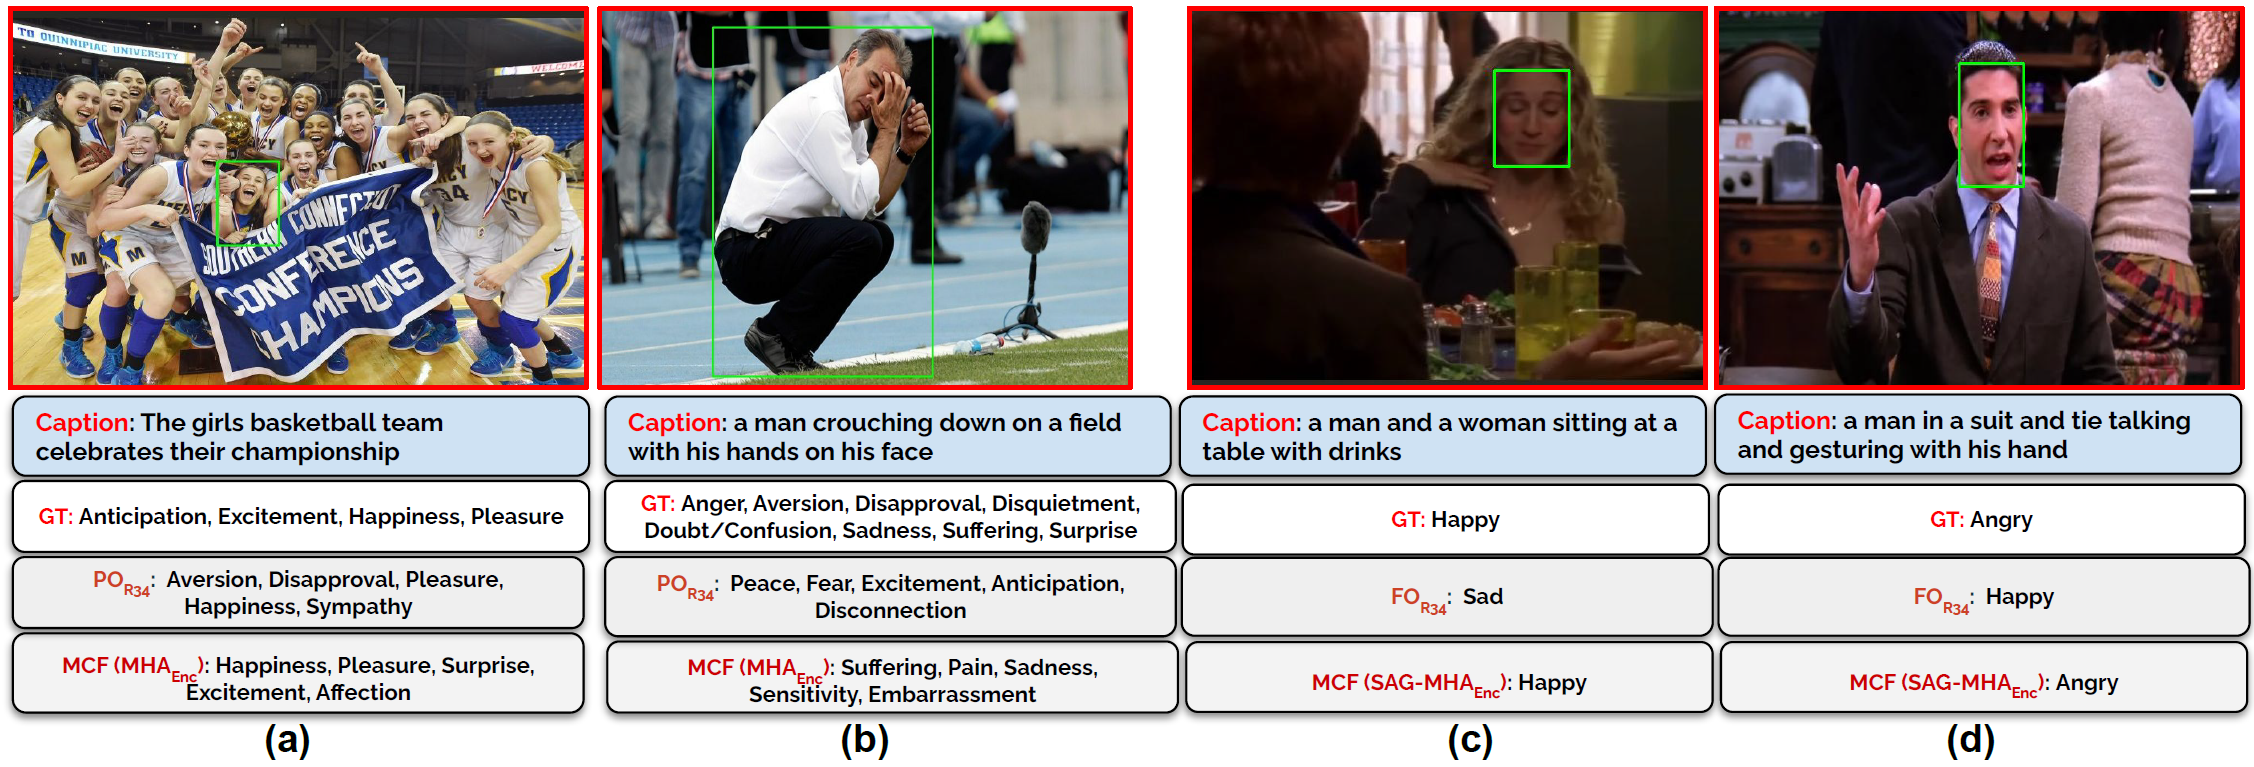
\includegraphics[width=\textwidth]{figures/EMOTIC_CAER_examples_updated.png}
    \caption{Examples (a) and (b) from EMOTIC showing comparisons between top-5 predictions of $PO_{R34}$ and MCF (MHA\textsubscript{enc}). Examples (c) and (d) from CAER-S showing comparisons between top predictions of $FO_{R34}$ and MCF (SAG-MHA\textsubscript{enc}) . $PO$: Person-only. $FO$: Face-only. $R_{34}$: Resnet34 fully finetuned. GT: Ground truth. Person or face instances marked by green bounding boxes}
    \label{qualfig}
\end{figure}

In Fig \ref{qualfig} (a) and (b), we can see that the inclusion of foreground context through captions like \textit{basketball team celebrating} and \textit{man crouching down with his hands on his face} results in consistent performance of MCF (MHA\textsubscript{enc}) as compared to $PO_{R34}$ (Resnet34 finetuned on person crops).  Similarly, for TV shows in Fig \ref{qualfig} (c) while the face crop based prediction from $FO_{R34}$ is \textbf{sad}, inclusion of foreground context with visual scene information gives a correct prediction for MCF (SAG-MHA\textsubscript{enc}). In Fig \ref{qualfig} (d), the act of \textit{gesturing with hand} enables MCF (SAG-MHA\textsubscript{enc}) to make a correct prediction (\textbf{Angry}) as compared to $FO_{R34}$ (Resnet34 finetuned on face crops).

\section{Limitations}

\begin{figure}[h!]
\centering
\subfloat[]{%
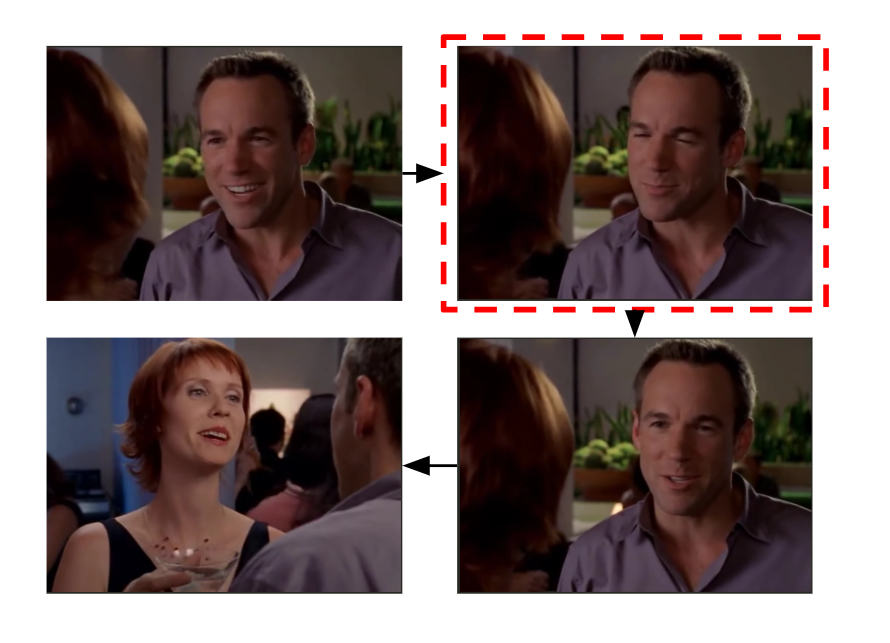
\includegraphics[width=0.5\textwidth]{figures/image_annotation.png}% 
\label{image annotation}
}
\subfloat[]{%
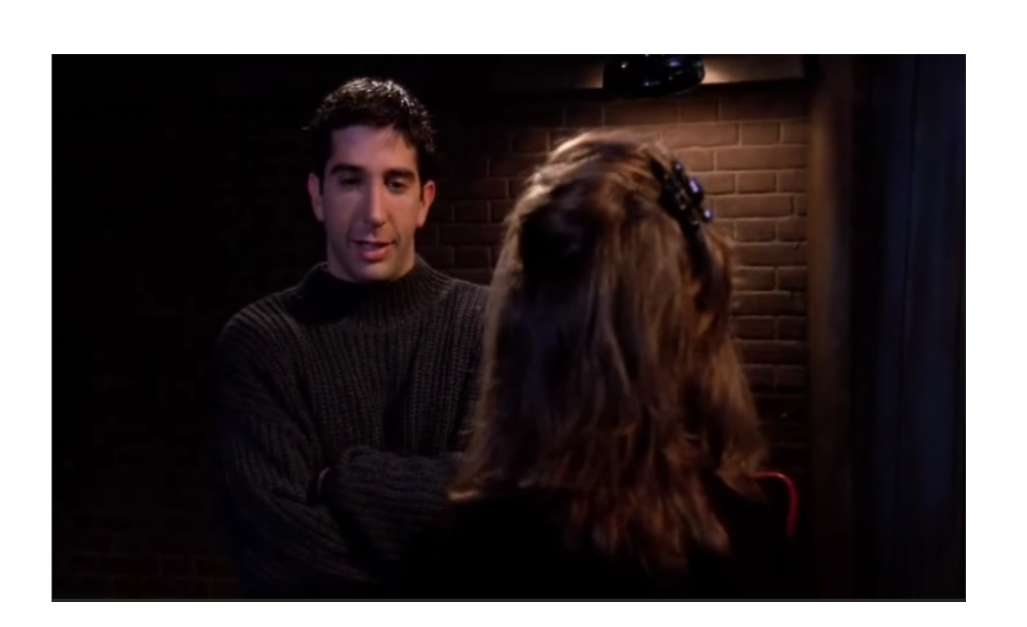
\includegraphics[width=0.5\textwidth]{figures/foreground_context.png}%
\label{foreground context}
}
\caption{(a) Lack of temporal information in image annotation (b) Incorrect foreground context predicted by OFA VLN \cite{wang2022ofa}: \textit{a man looking at a girl in a mirror}}
\label{temporal information and incorrect foreground}
\end{figure}

For image-based datasets like CAER-S, a lack of temporal information provides an ambiguous setting for marking the affective state of the person. For the red marked frame in \textbf{(a)}, it is difficult to infer that the person is feeling happy since the eyes and mouth are closed. However, if the interactions are taken into account, it can be seen that the person is feeling happy. Further, in the case of foreground context, OFA VLN provides the description: \textit{a man looking at a girl in a mirror}. This indicates that there are cases where the foreground context might not be captured correctly by pretrained vision language models.

% In this work, we explore the role of contextual information in estimating human emotions with respect to the domains of natural scenes (EMOTIC) and TV shows (CAER-S). Since multimodal-VLN models are pretrained on large-scale image-text pairs from the web, we utilize their capabilities to obtain foreground context information in terms of descriptive captions. Further, we propose a purely attention-based multimodal context fusion (MCF) module to combine person-specific information with the visual scene and foreground context representations. Future work involves the extension of the MCF module to include geometric aspects of person context including pose information and evaluation using media-centered data like movies and advertisements.

\section{Conclusion}



\chapter{Advertisement video understanding through the lens of temporal context}

In this chapter, we will explore the role of temporal context in macro-level content understanding of dynamic sources, i.e., videos. Specifically, we consider advertisement videos due to their unique narrative structures of multiple short-term temporal context changes that are linked by a longer narrative thread. In order to study the context-driven approaches, we introduce a new ads-specific benchmark called \textbf{\textit{MM-AU}} with salient narrative-driven tasks for macro-level understanding i.e., topic categorization, tone transition, and social relevance. 

\section{Video Understanding}

Video Understanding aims to identify semantic elements from videos, including: \textit{environment}, \textit{objects}, \textit{actions}, \textit{events}, \textit{attributes}, \textit{concepts/themes} \cite{diba_large_2020}. Recognition of the semantic elements requires processing temporal context across different time scales, including short-term and long-term. As shown in Fig \ref{short term and long term context}, the short-term context in videos centers around visible human actions for a limited duration. However, long-term context consists of an integrated narrative spanning across multiple short-term context changes. In the case of movies, the long-term context can even span the entire duration of the movie. In this work, we primarily look at advertisement videos due to their unique narrative structure consisting of multiple short-term context changes along with long-term linkage within a limited time frame.

\begin{figure}[h!]
\centering
\subfloat[]{%
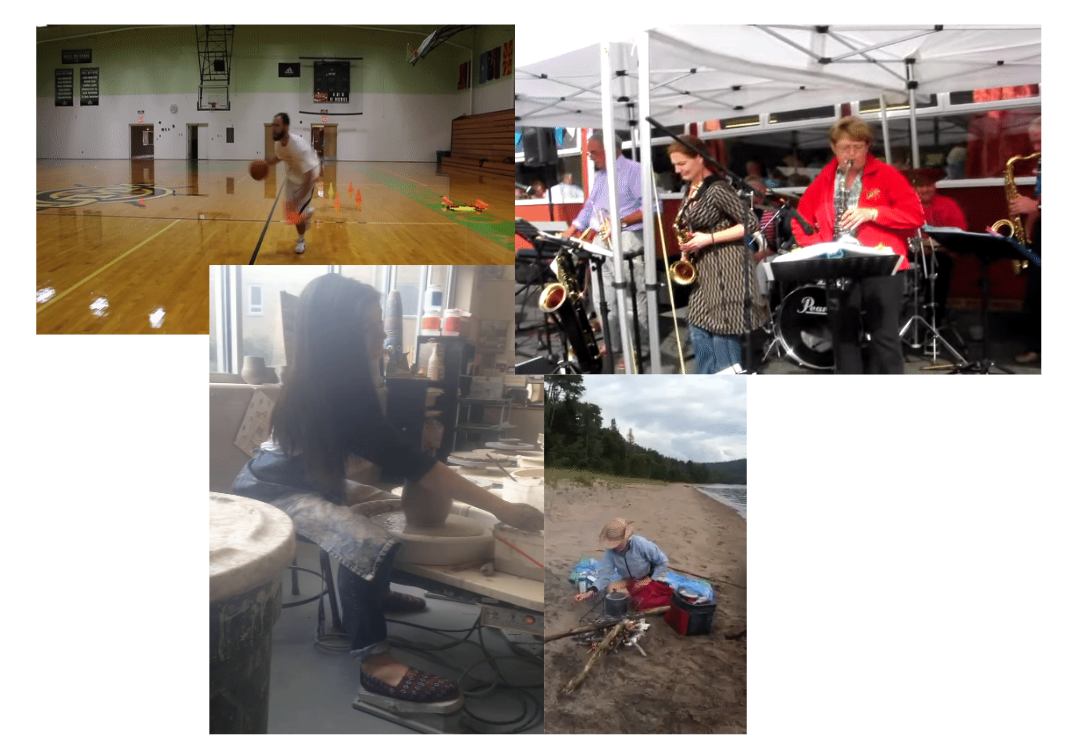
\includegraphics[width=0.5\textwidth]{figures/short_context_pictures.png}% 
\label{short context}
}
\subfloat[]{%
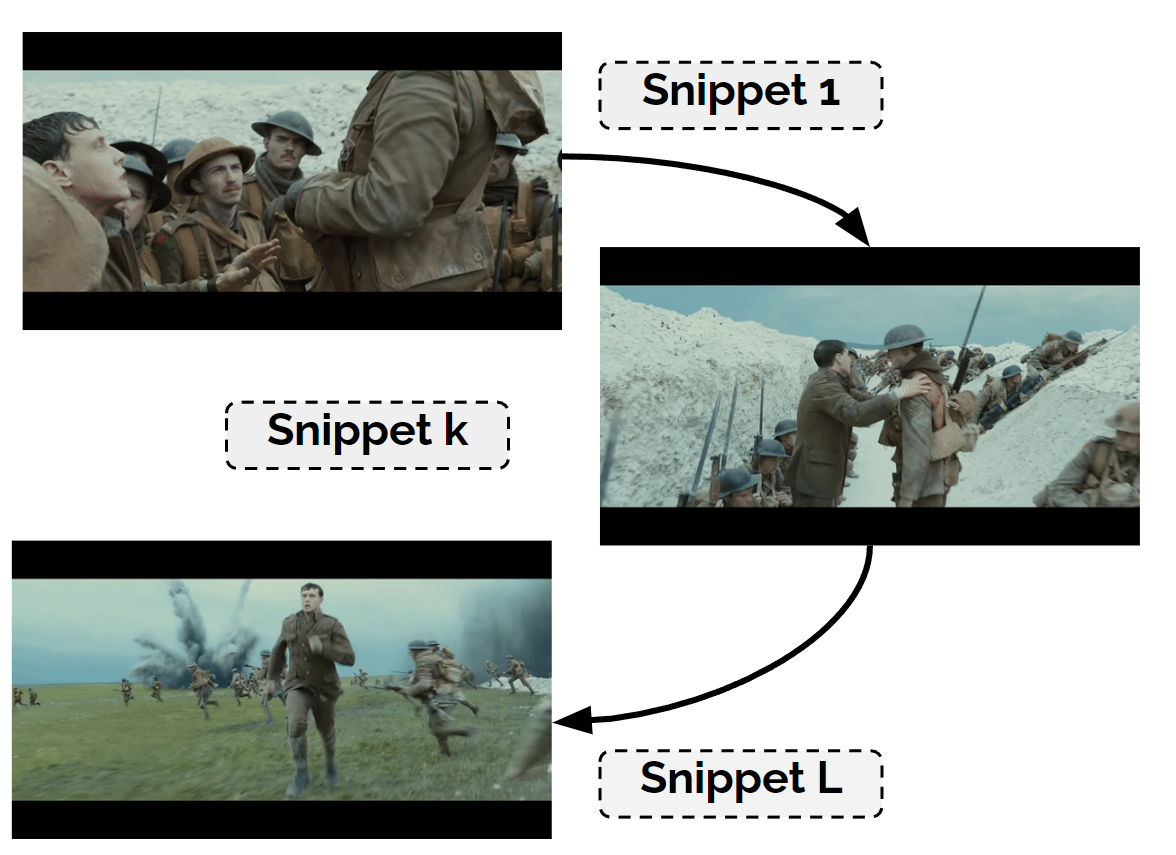
\includegraphics[width=0.5\textwidth]{figures/long_context_picture.png}%
\label{long context}
}
\caption{(a) Short-term context centered on human actions (b) Long-term context in movies useful for narrative understanding}
\label{short term and long term context}
\end{figure}

\section{Advertisements - Context transitions}

In terms of context transitions, advertisements lie between action-oriented short videos and feature-length movies. In Fig \ref{ads_structure_set}, we can see that multiple short-term context changes are happening due to the following sequence of activities/interactions:
\begin{itemize}
\item Police activity starting
\item Police chief gathering 
\item Police vehicles are getting destroyed
\item Children playing with toys 
\end{itemize}
From the sequence of events, it can be inferred that even though the short-term temporal information indicates negative situations, the overall theme revolves around toys for kids.
Thus, the temporal context information needs to be processed both locally and globally for a holistic understanding of ads at macro-level. 

\begin{figure}[h!]
\centering
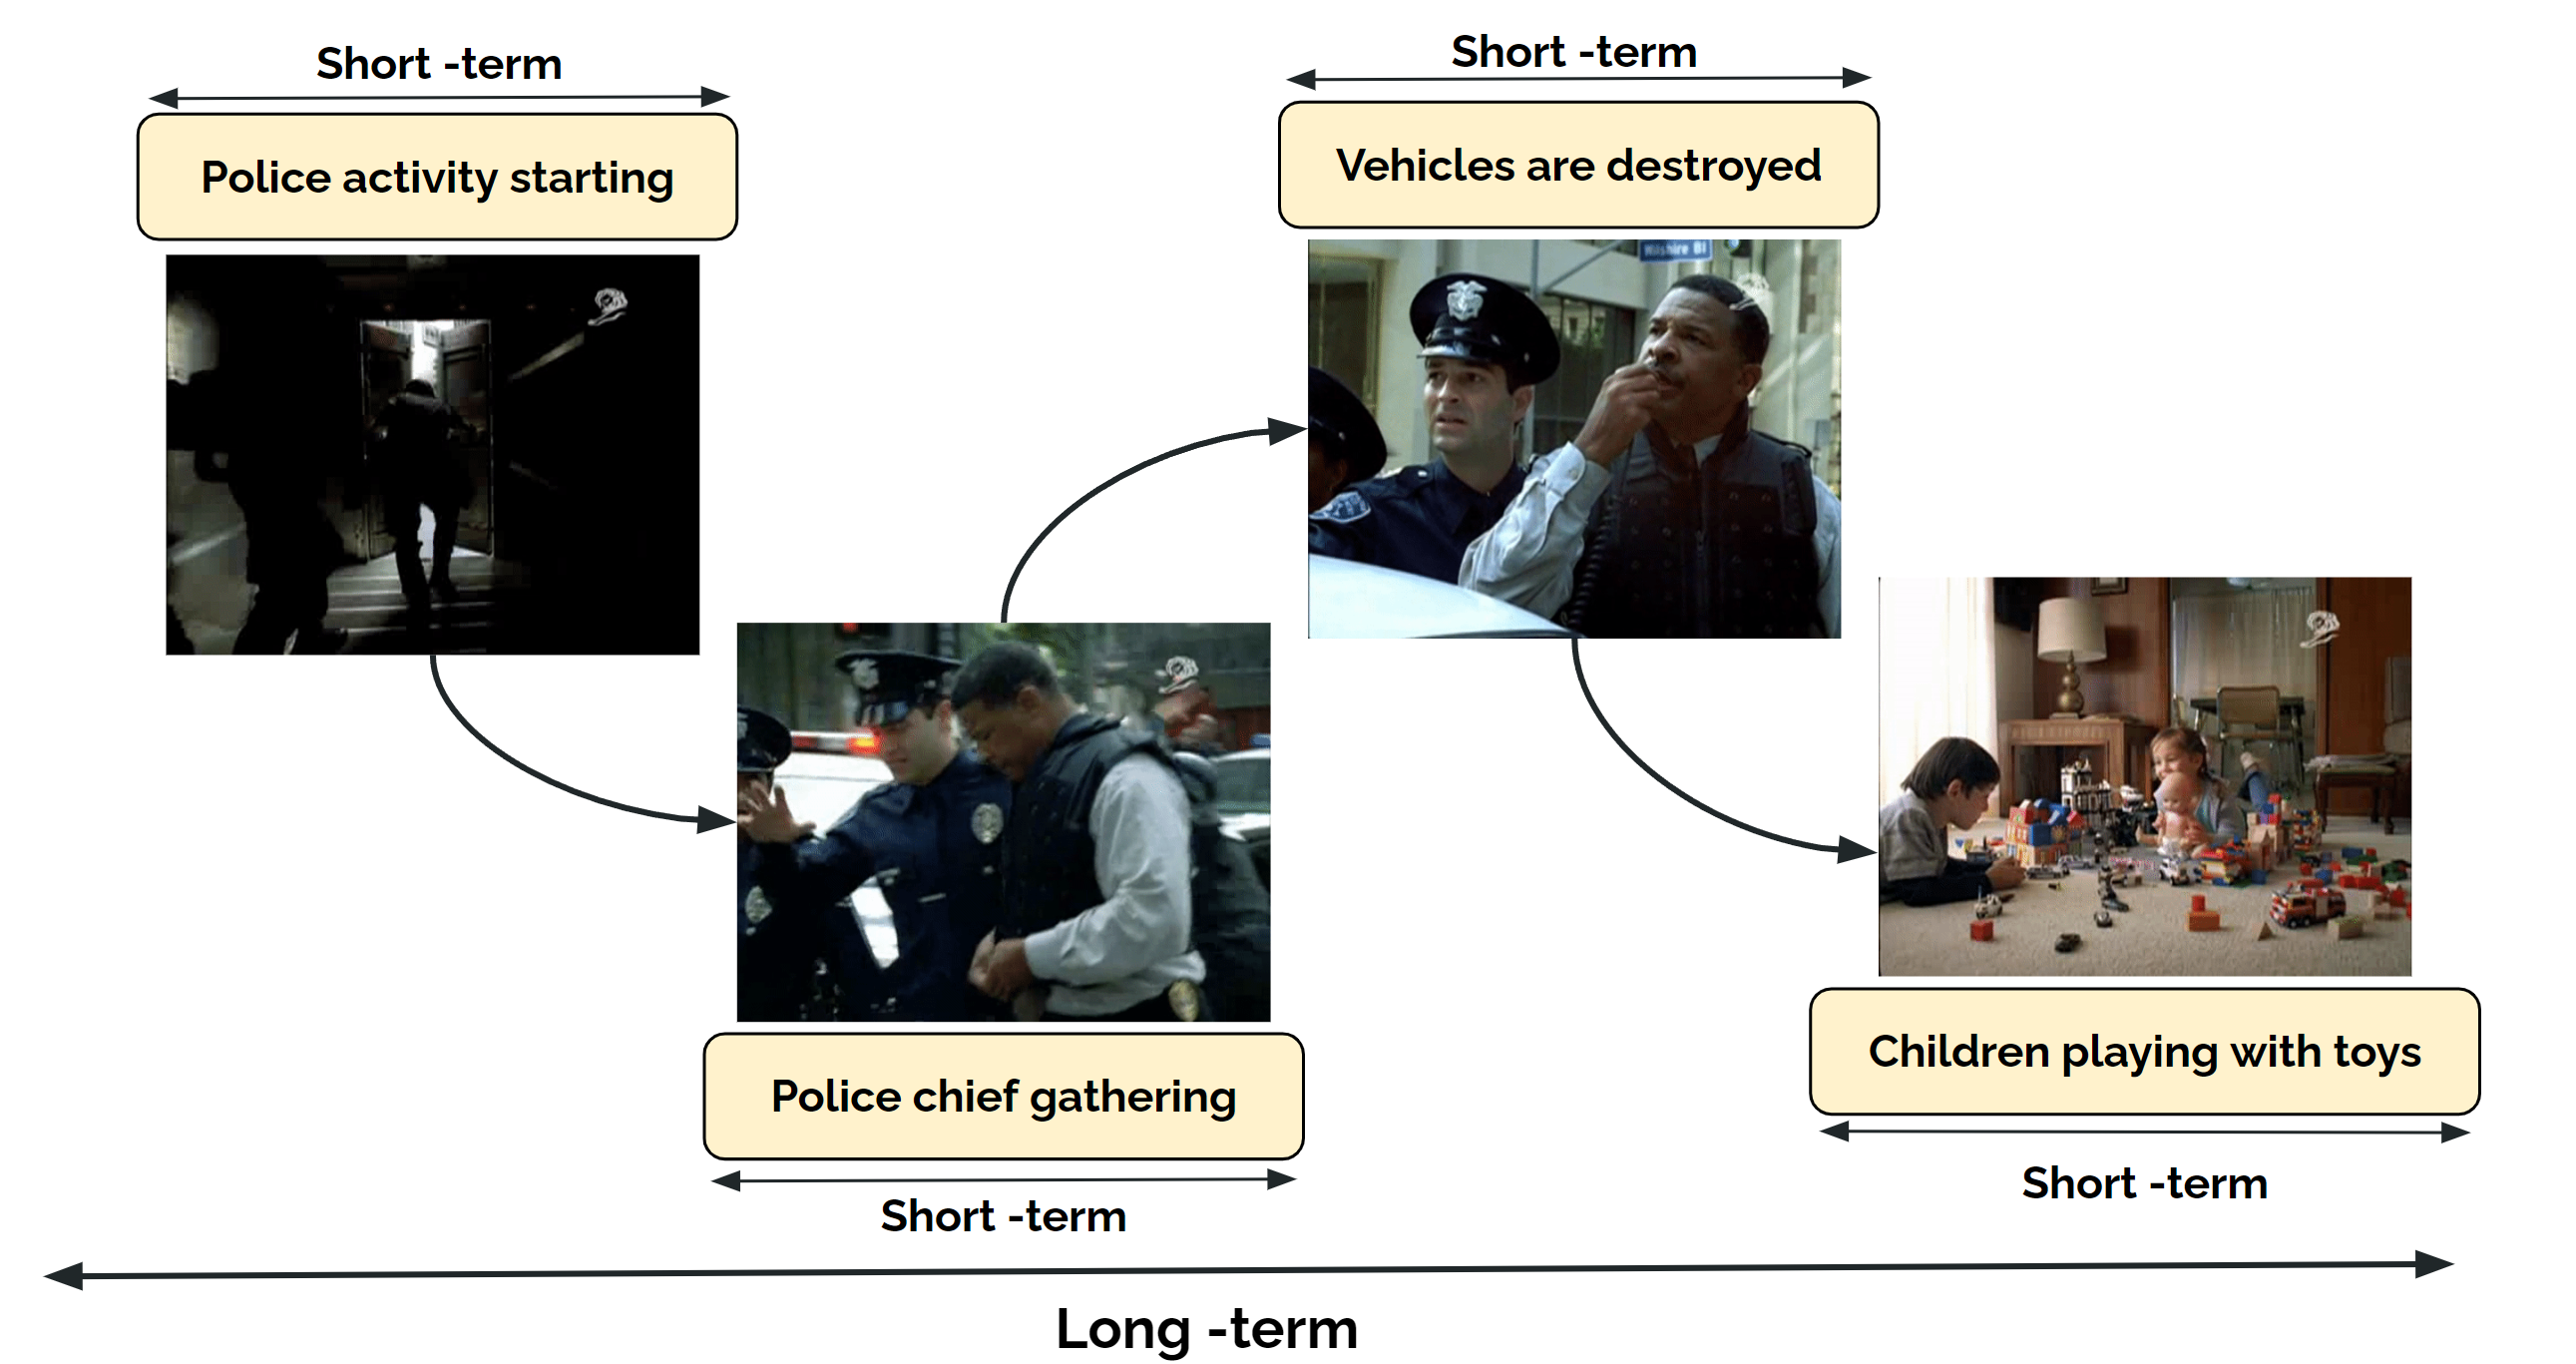
\includegraphics[width=\textwidth]{figures/ads_structure_figure.png}
\caption{Structure of advertisement video with multiple short-term context changes and overall long-term linkage}
\label{ads_structure_set}
\end{figure}

\section{Advertisements as medium}
As a primary media source for disseminating information, advertisements (ads for short) have been utilized to promote products or convey messages about extant social or political issues. The utility of advertisements as a media source has been amplified by the wide variety of platforms like radio, television, newspaper print, video streaming, and social networking sites, presenting significant influences, whether direct or indirect, to viewers from diverse backgrounds \cite{Pardun}. As shown in Fig \ref{ads_structure_set}, The rising importance of advertisements in the current socio-economic scenario is evident from the expected increase in media ad spending from 225.79 in 2020 to 322.11 billion dollars in 2024.

\begin{figure}[h!]
\centering
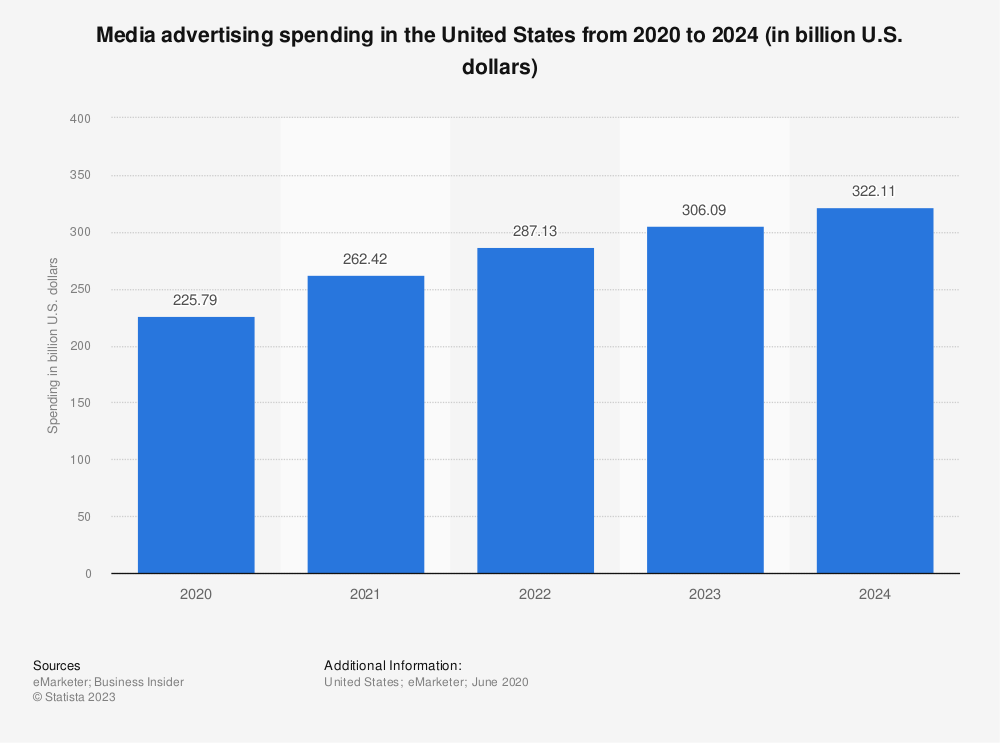
\includegraphics[width=0.9\textwidth]{figures/statistic_id272314_advertising-spending-in-the-us-2020-2024.png}
\caption{Increase in demand for advertisements over last 4 years}
\label{ads_structure_set}
\end{figure}

\section{Advertisements - Narrative driven tasks and challenges}

Objectively understanding the rich content in ads and their impact on the viewer experience and behavior is hence of great interest. However, in enabling computational media understanding \cite{CMI}, advertisements present unique challenges in the form of condensed narrative structures \cite{Kim2017WhyNA}. Due to their relatively short duration when compared to feature-length movies, an advertisement video showcases a particular narrative structure in a tightly integrated sequence with different formats, including slice-of-life \cite{Mick1987TowardAS}, drama \cite{Leong1994UsingDT}, and transformational \cite{Puto1984InformationalAT}. Further, reasoning about the narrative structure requires a multi-scale understanding of the underlying topic and fine-grained elements, including the sequence of events (of characters and interactions) and related messages. As shown in Fig~\ref{introfig}, the key elements associated with the narrative structure of ads and related challenges are listed as follows:

\begin{figure}[h!]
\centering 
    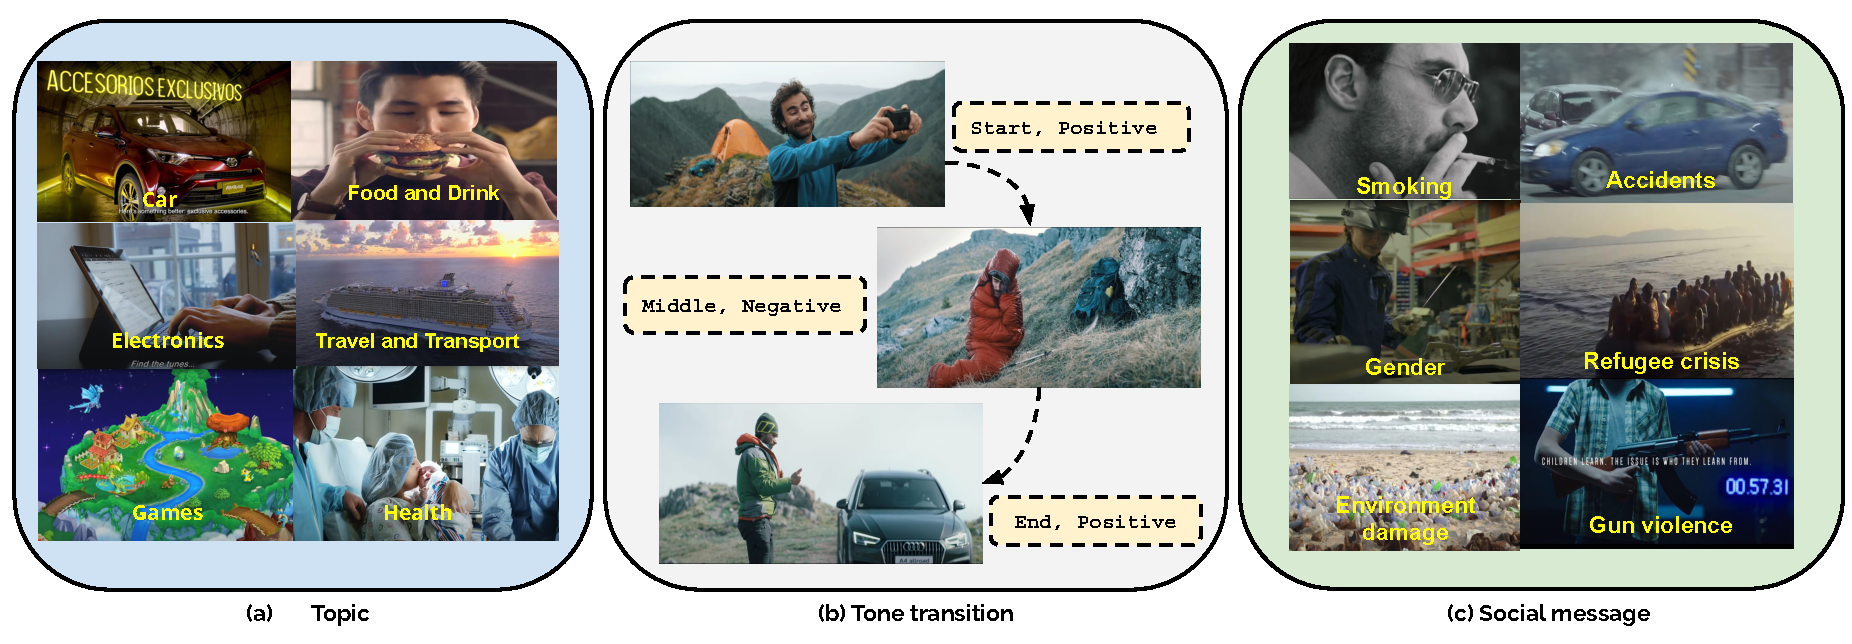
\includegraphics[width=0.8\textwidth]{figures/Task_outline_1_Topic_TT_SM.pdf}
  \caption{Schematic diagram showing illustrative examples of various tasks in the MM-AU (Multi-modal ads understanding) dataset. Multimodal understanding of ads along the lines of (a) Topic categorization (18 classes) (b) Tone transition (c) Social message detection i.e. Absence/Presence of social message}
  \label{introfig}
\end{figure}

\textbf{\underline{Topic}}: understanding enables personalized categorization and retrieval for customers along with key insights into the representation of genders \cite{google-diversity} and different demographic groups with respect to target classes like healthcare, retail, travel, etc. Topic categorization involves the handling of both inter and intra-topic diversity between the videos in terms of human-object interactions and a wide variety of items/products, as shown in Fig~\ref{introfig} (a). 

\textbf{\underline{Tone transition}}: Affective tone associated with an advertisement video refers to the perceived feeling by a viewer \cite{Veer2008HowTT}. Associating the appropriate tone with an ad enhances its persuasiveness, thus enabling the associated brand to expand its reach to a wide range of customers. While the positive tone centers around optimistic elements associated with hope and success \cite{Brooks2020ExploringAO}, portrayals of negative tone are tied to sad narratives involving fear and suffering. However, due to the narrative structure, the perceived affective tone exhibits transitions during the duration of an advertisement video, accompanied by changes in visuals and background music.  In Fig~\ref{introfig} (b), the video starts on a positive note with a happy person taking a picture, followed by a perceived negative tone in the middle due to the suffering of the person. The advertisement ends on a positive note, with the person being saved by an incoming vehicle.\\

\textbf{\underline{Social message}}: Advertisements act as a major source of information about pressing social issues for consumers. Brands conveying messages about various social issues, including but not limited to gender inequalities, racial discrimination, and environmental conservation, are viewed favorably by consumers across different age groups \cite{Brooks2020ExploringAO}. In terms of advertisement videos, social message portrayal is characterized by a huge diversity in depiction, as shown in Fig~\ref{introfig} (c) due to underlying categories like smoking, accidents, gun violence etc.

In this work, we introduce a multilingual multimodal benchmark called \textbf{\textit{MM-AU}} for the macro-level understanding of advertisement videos across the tasks of topic categorization, social message, and tone transition detection. Due to the inherent structure of the ads involving transitions in temporal context driven through multiple modalities, we propose context-guided attention mechanisms for the previously mentioned macro-level tasks. Our contributions can be listed as follows:

\begin{itemize}
    \item \textbf{\underline{Topic classification:}} We merge existing taxonomies for topic annotations from prior ads datasets and publicly available websites like {Ads of world}\footnote{https://www.adsoftheworld.com/} to obtain a condensed set of topic labels for the advertisement videos.
    \item \textbf{\underline{Tone Transition detection:}} We introduce a novel benchmark task of tone transition detection in advertisement videos by obtaining crowdsourced feedback from human annotators.
    \item \textbf{\underline{Social message detection:}} We provide weak human expert-based labels for detecting the presence/absence of social messages in advertisement videos.
    \item \textbf{\underline{Language-based reasoning:}} We explore zero-shot baselines for the three benchmark tasks through applications of large-language models on ad transcripts.
    \item \textbf{\underline{Context guided attention:}} We provide multiple context-guided attention baselines to benchmark the performance for the three macro-level tasks (topic classification, transition detection, and social message) and highlight future possibilities of explorations.
\end{itemize}
\section{Related work}

\textbf{Narrative understanding:} 
Narratives \cite{Fisher1987HumanCA} play an important role in enabling effective human communication and organizing the daily sequence of events. Advertisements centered on narratives \cite{Escalas1998ADVERTISINGNW} influence consumers by providing a concrete story arc centered around specific themes, protagonists, and their actions. Kim et al. \cite{Kim2017WhyNA} introduced an integrated theory of understanding narratives in advertisements based on key variables like emotic response, ad hedonic value, ad credibility, and perceived goal facilitation. Lien et al. \cite{Lien2013NarrativeAT} explored narrative ads from the lens of persuasion and the relationship with different advertisement mediums - verbal or visual. In the realm of computational narrative understanding, prior works have focused on language-based approaches for marking high-level structures in short stories \cite{Li2017AnnotatingHS}, most reportable events (MRE) in Reddit comment threads \cite{Ouyang2015ModelingRE} and primary processes in movie scripts, newspaper articles, etc \cite{Boyd2020TheNA}.\\
\textbf{Affect modeling in videos:}
Advertisement brands tend to invoke emotional reactions \cite{Holbrook1984TheRO} in viewers by influencing their actions i.e., purchasing a particular product. In the domain of television commercials, a combination of physiological, symbolic, and self-report measures was explored in \cite{Micu2010MeasurableEH} to determine the emotional responses of viewers. The role of facial expressions in decoding the preferences of viewers, including purchase intent, and smile responses, has been explored through large-scale studies in \cite{McDuff2014PredictingAL}, \cite{Teixeira2014WhyWA}. Apart from facial expressions, the role of CNN-based audio-visual and EEG descriptors from the viewers has been explored in a multi-task setup \cite{Shukla2017AffectRI,Shukla2017EvaluatingCV,Shukla2019RecognitionOA} for arousal and valence prediction in advertisement videos. Existing video-based affect datasets like DEAP \cite{Koelstra2012DEAPAD}, VideoEmotion \cite{Jiang2014PredictingEI} also focused on single arousal, valence, and dominance ratings as well as discrete emotion labels for music and user-generated videos, respectively.\\
In the domain of continuous affect modeling, datasets with frame-level annotations have been introduced across a wide variety of domains, including naturalistic and induced clips (HUMAINE \cite{DouglasCowie2007TheHD}), movies (COGNIMUSE \cite{Zlatintsi2017COGNIMUSEAM}, LIRIS-ACCEDE \cite{Baveye2015LIRISACCEDEAV}) and online videos (EEV \cite{Sun2020EEVDP}). Further extensions of continuous affect modeling based on independent and self-reports have been explored for daily emotional narratives in SENDv1 dataset \cite{Ong2019ModelingEI}. For advertisements, climax annotations (presence + rough timestamps) were provided by human annotators on a subset of the Video Ads dataset \cite{Hussain2017AutomaticUO} in \cite{Ye2018StoryUI} along with climax-driven modeling strategies to predict sentiment labels at the video level. 
In our proposed benchmark \textbf{\textit{MM-AU}}, based on the standard definition in \cite{Brooks2020ExploringAO}, we ask human annotators to denote the perceived tone in the advertisement video across segments approximately marking the start, middle, and end. The perceived tone transition enables tracking of the narrative dynamics in advertisement videos by considering the interactions between various contextual streams through different modalities, i.e. audio, visual, and narrations/spoken interactions (through transcripts).\\
\textbf{Advertisement benchmarks:} 
\begin{table*}[h!]
\centering
\resizebox{\textwidth}{!}{
\begin{tabular}{|c|c|c|c|c|c|c|c|c|}
\hline
\textbf{Dataset}       & \textbf{Annotation type} & \textbf{Duration} & \textbf{\#Samples} & \textbf{\#Shot} & \textbf{\#Class}                     & \textbf{Modalities}      & \textbf{Languages}                   & \textbf{Tasks}                      \\ \hline
Video Ads Dataset (I)  & H                        & NA                & 64832              & NA              & 38 (T), 30 (S), AR (OE), H(2), Ex(2) & Images                   & English                              & Image level classification          \\ \hline
Video Ads Dataset (V)  & H                        & 144.87            & 3477               & NA              & 38 (T), 30 (S), AR (OE), H(2), Ex(2) & Video                    & English                              & Video level classification          \\ \hline
Tencent-AVS            & H                        & 142.1h            & 12k                & 121.1k          & 25 (Pr), 34 (St), 23 (Pl)            & Video/Audio/ASR/OCR              & Chinese and English                  & Scene level classification          \\ \hline
Ads-persuasion dataset & H + AL                   & NA                & 3000               & NA              & 21 (PS)                              & Images                   & English                              & Image level classification          \\ \hline
E-MMAD                 & SG descriptions          & 1021.6 h          & 120984             & NA              & 4863 (PC)                            & Video                    & Chinese and English                  & Video level captioning              \\ \hline
\textbf{MM-AU}         & \textbf{H + SA}          & \textbf{147.8h}   & \textbf{8399}      & \textbf{216.4k} & \textbf{18 (T), 3 (Tone), 2 (SM)}    & \textbf{Video/Audio/ASR} & \textbf{Multilingual (65 languages)} & \textbf{Video level classification} \\ \hline
\end{tabular}
}
\vspace{5mm}
\caption{Comparison of \textbf{\textit{MM-AU}} with other available advertisement benchmarks across different modalities.  \underline{Annotation type:} \textbf{H}: Human annotation, \textbf{AL}: Active Learning, \textbf{SA}: Semi-automatic, \textbf{SG}: Store generated. \underline{Duration:} \textbf{NA}: Not applicable for images; Mentioned in hours(h). \underline{\#Samples:} Number of video clips or images. \underline{\#Shot:} \textbf{NA}: Not applicable for images; Number of shots detected from all the video samples. \underline{\#Class:} \textbf{T:} Topic, \textbf{S:} Sentiment, \textbf{OE:} Open-Ended, \textbf{H:} Humor, \textbf{Ex:} Exciting, \textbf{Pr:} Presentation, \textbf{St:} Style, \textbf{Pl:} Place, \textbf{PS:} Persuasion strategy, \textbf{PC:} Product categories, \textbf{SM:} Social messages}
\label{Overview}
\end{table*}

While there has been progress in terms of movie understanding due to the introduction of large-scale multimodal benchmark datasets like Condensed Movies \cite{bain2020condensed}, MovieNet \cite{huang2020movienet}, MAD \cite{Soldan_2022_CVPR}, Movie-cuts \cite{Pardo2021MovieCutsAN}, MovieCLIP \cite{Bose_2023_WACV} and SAM-S \cite{Hebbar2023ADF}, only few benchmarks have focused on large-scale understanding of advertisements across broad and fine-grained content. Hussain et al. \cite{Hussain2017AutomaticUO} introduced the benchmark Video-Ads dataset to facilitate understanding of images and videos along the lines of broad topics, induced sentiments, and action/intent reasoning. The images in the Video-Ads dataset were utilized in \cite{Singla2022PersuasionSI} for computational modeling of persuasion across 21 categories in marketing domain. Regarding large-scale ads understanding, Tencent-AVS dataset \cite{Jiang2022TencentAA} was proposed to enable multi-modal scene level categorization into semantic classes like presentation, places and styles. While the previously mentioned datasets focused on classification tasks, E-MMAD \cite{Zhang2022AttractMT} introduced the task of informative caption generation from advertisements across 120k e-commerce videos.
\\
\textbf{\textit{MM-AU}}, our curated multilingual dataset utilizes publicly available videos from Ads of the World along with a subset from Video-Ads dataset and an in-house video catalog from Cannes Lion archive \cite{cannes-lions}. We provide 18 broad topic categories by combining existing taxonomies (Cannes Lion, Ads of World, and Video-Ads dataset). Further, we rely on human expert annotators to label transitions in perceived tone along with the absence/presence of social messages in 8.4K advertisement videos. A comparative overview of \textbf{\textit{MM-AU}} and other advertisement datasets is shown in Table \ref{Overview}.\\
\textbf{Semantic video understanding:}
Existing large-scale video datasets including Kinetics\cite{Carreira2017QuoVA}, Moments-in-time \cite{Monfort2018MomentsIT}, ActivityNet \cite{Heilbron2015ActivityNetAL}, AVA \cite{Gu2017AVAAV} have focused mainly on classifying entity driven actions from in-the-wild short videos. Higher-level semantic labels beyond actions like topics, concepts, events, and video types were exploited for large-scale video-level categorization in datasets like Youtube-8M \cite{AbuElHaija2016YouTube8MAL}, Holistic-visual understanding (HVU) \cite{diba2020large} and 3MASSIV \cite{Gupta20223MASSIVMM}. Our proposed benchmark \textbf{\textit{MM-AU}} explores the domain of semantic video understanding in ads by considering broad categories like topic, presence/absence of social message, and fine-grained affective labels of perceived tone transition.\\
\textbf{Multimodal representation learning:} Multimodal representation learning \cite{Liang2022FoundationsAR} centers around the fusion of information from different modalities at multiple scales, including early, late, and mid-fusion. Prior works related to ads have utilized multimodal-LSTMs \cite{Vedula2017MultimodalCA}, segment-level autoencoders \cite{SomandepJointenc} or joint cross-modal embedding \cite{Ye2019InterpretingTR} approaches for learning multimodal representations for a variety of tasks. With the advent of transformer \cite{transformers} based multimodal models like PerceiverIO \cite{Jaegle2021PerceiverIA}, attention bottlenecks\cite{nagrani2021attention}, and VATT \cite{Akbari2021VATTTF}, information fusion at the input token space, followed by joint encoders, have become more prevalent. A multi-task attention-based approach was explored in \cite{LookReadFeel} for jointly predicting topic and sentiment labels associated with advertisement images. A NextVLAD \cite{Lin2018NeXtVLADAE} based approach \cite{Weng2021AMF} combined with global-local attention was utilized for predicting scene-specific labels in the Tencent \cite{Jiang2022TencentAA} ads benchmark dataset.
\section{MM-AU benchmark}
\subsection{Data sources}
We consider multiple ads-specific sources for curating our proposed MM-AU dataset. As a primary source, we consider Ads-of-the-world (AOW)\footnote{https://www.adsoftheworld.com/} video hosting website since it contains a richly-curated catalog of ads in various formats like film, print, digital, and video spanning across multiple countries. As auxiliary sources, we consider additional videos from the Cannes Lion Film Festival archive and Video-Ads dataset \cite{Hussain2017AutomaticUO}. We filter the videos based on unique video ids associated with their public links to ensure no duplicates across three sources. The share of different sources in curating the combined list of 8399 advertisement videos is shown in Fig~\ref{ads_sources}
\begin{figure}[h!]
    \centering
    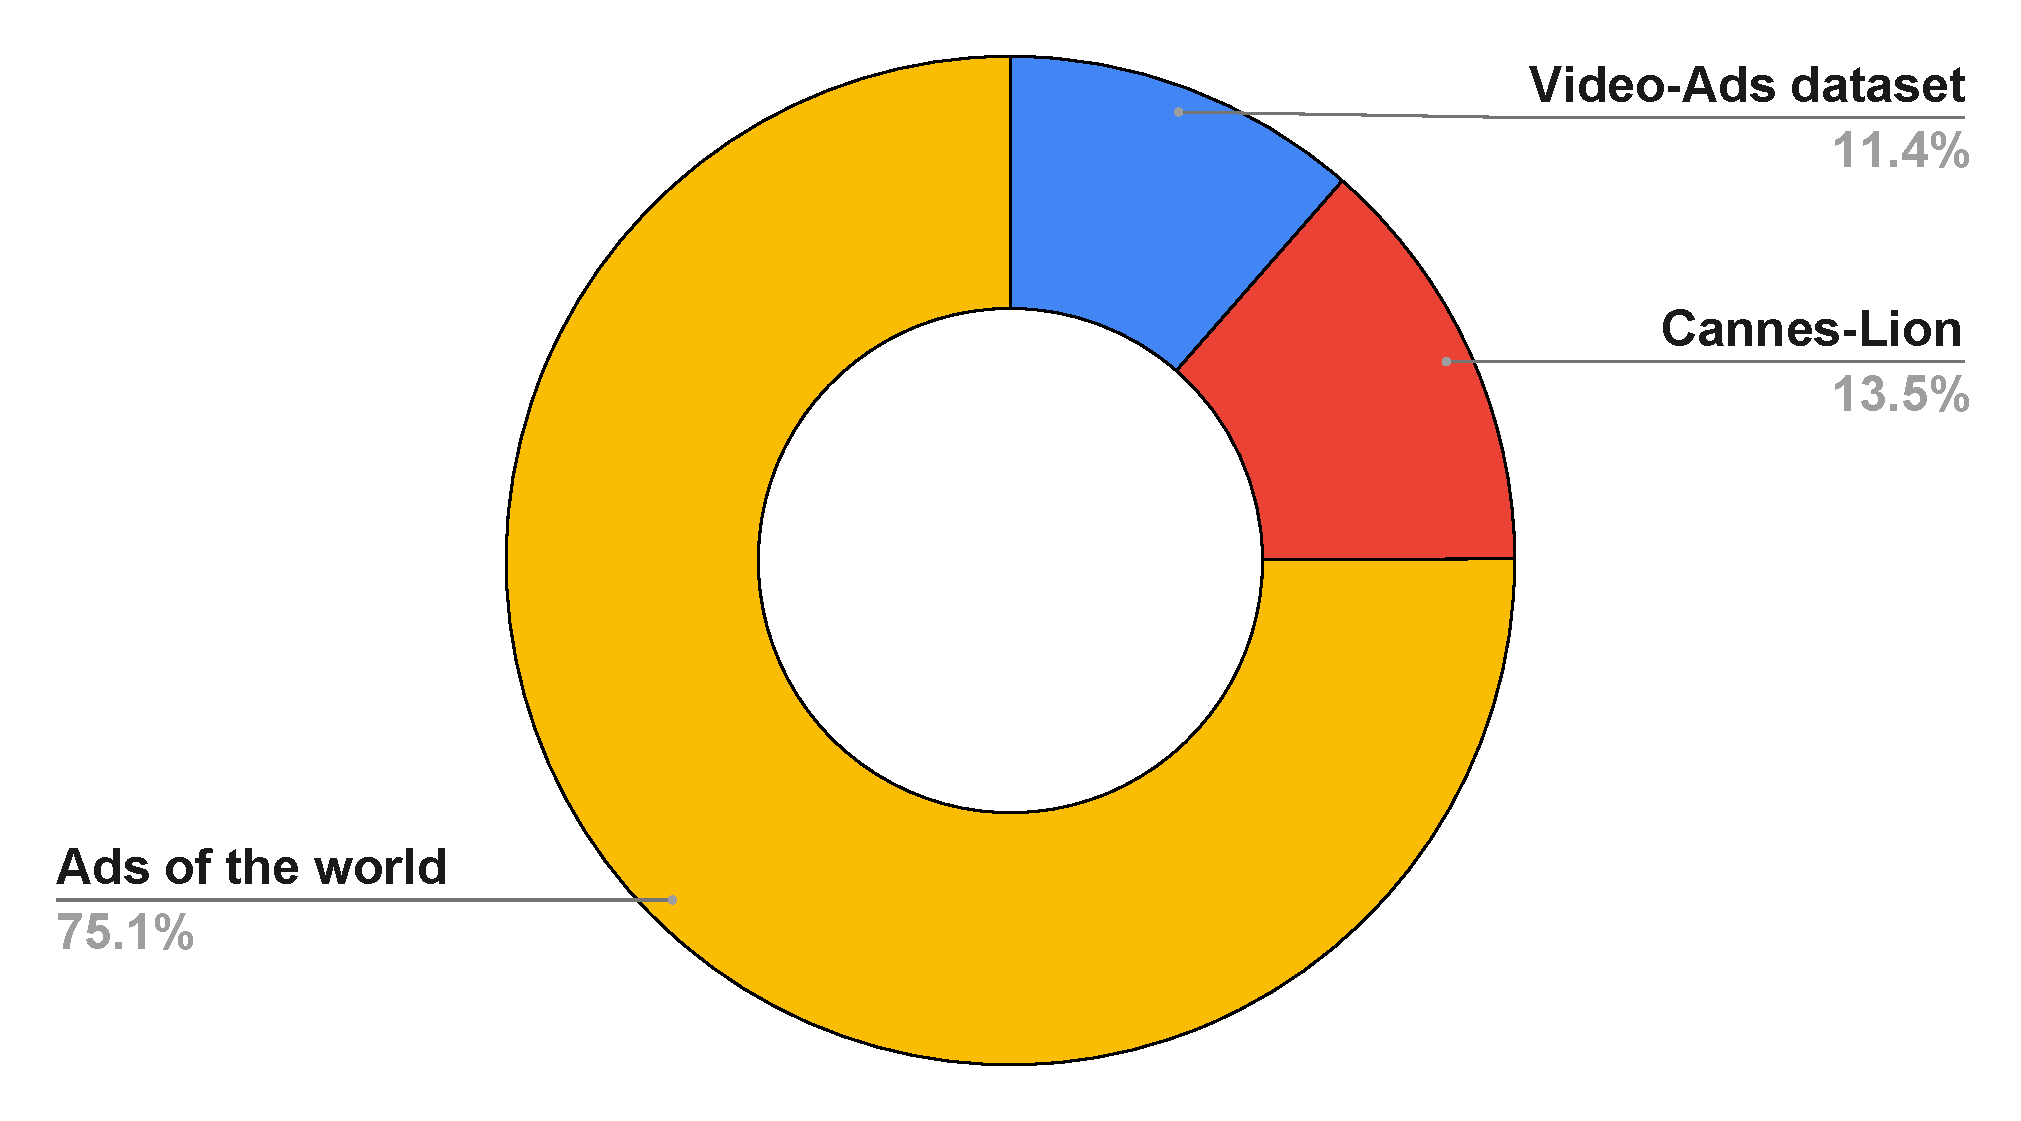
\includegraphics[width=0.8\textwidth]{figures/data_sources_distribution.pdf}
    \caption{Share of different ad sources in MM-AU dataset. Ads of the world (6304 videos), Cannes Lion (1135), Video-Ads dataset (960) }
    \label{ads_sources}
\end{figure}

\subsection{Human expert-driven annotations}
We employ a semi-automatic process for tagging the advertisement videos with broad topic categories. For the detection tasks of tone transition and social message, we use Amazon Mechanical Turk \footnote{https://www.mturk.com/} to obtain responses from a pool of 36 human annotators. 
For selecting a pool of workers with the requisite expertise, we hosted an initial pilot study where the workers are instructed to mark the tone transition labels and presence/absence of social message in the given set of videos. Further, in the final annotation phase, three annotators independently annotate each sample for the tone-transition and social message detection tasks. 
The annotation process details associated with the respective tasks are listed below:\\
\textbf{\underline{Tone transition:}} The annotators are instructed to mark the perceived tone labels associated with the start, middle, and ending segments of the advertisement videos. To reduce the burden associated with the task, no instructions are provided to mark the timestamps associated with the respective segments. 
\begin{figure*}[h!]
    \centering
    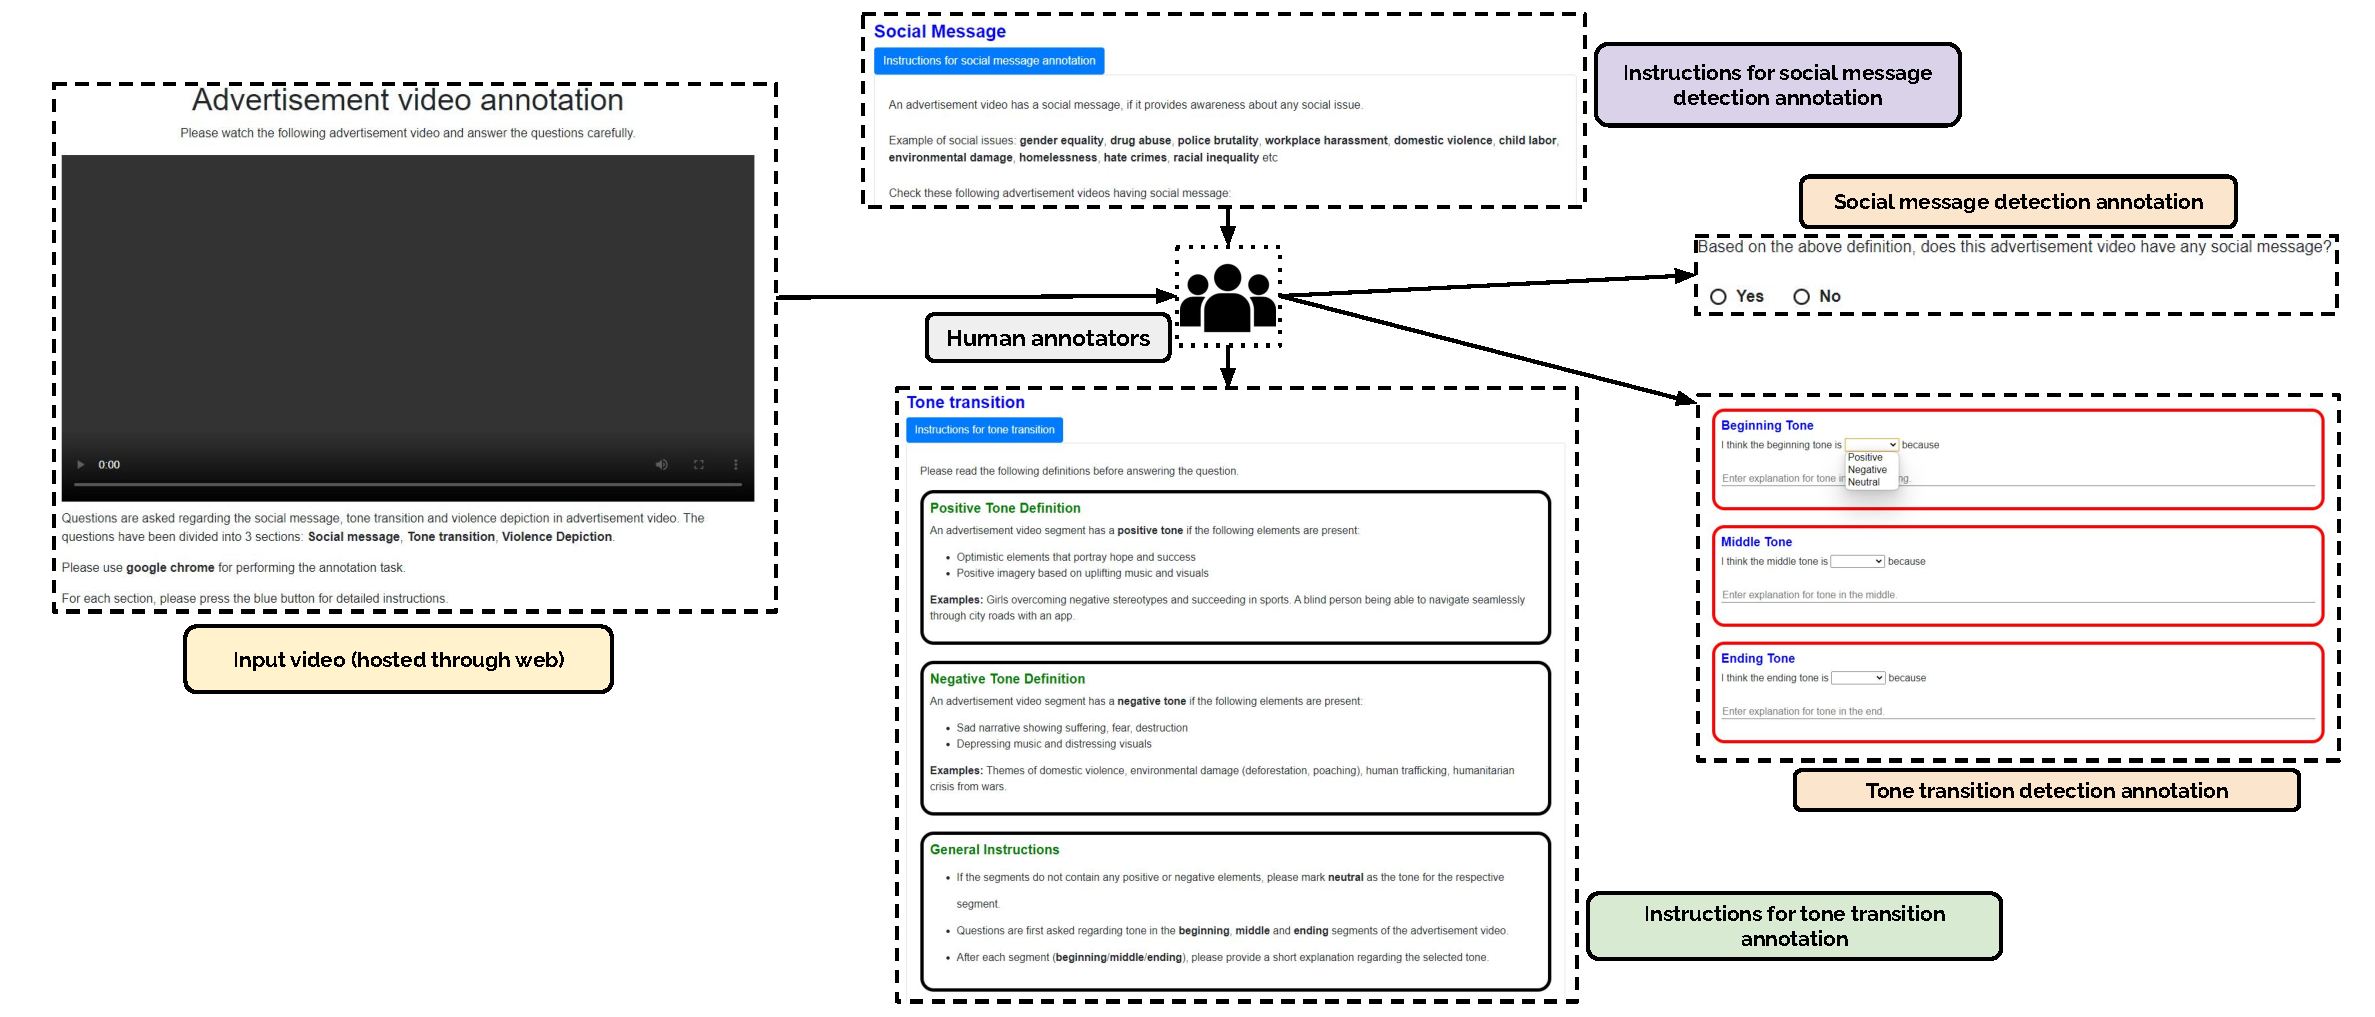
\includegraphics[width=\textwidth]{figures/Annotation_Flow_Part_2_updated.pdf}
    \caption{Outline of the annotation framework for tone transition and social message detection problem}
    \label{annot_framework}
\end{figure*}
Based on the tone definition considered in \cite{Brooks2020ExploringAO}, we provide the following descriptions to aid the annotation process:
\begin{itemize}
    \item \textbf{Positive tone:} An advertisement video segment has a positive tone if it contains: \textit{optimistic elements portraying hope and success} or \textit{positive imagery based on uplifting music and visuals}. Examples include girls overcoming negative stereotypes and succeeding in sports or a blind person being able to navigate easily through city roads by using an app.
    \item \textbf{Negative tone:} An advertisement video segment has a negative tone if it contains: \textit{sad narrative showing suffering, fear, destruction} or \textit{depressing music and distressing visuals}. Salient themes associated with negative tone include domestic violence, environmental damage, human trafficking, crisis from wars etc.
\end{itemize}
If a segment does not contain the above-mentioned characteristics, the annotators are instructed to mark the perceived tone as neutral. To determine the reasoning involved in marking the tone labels associated with the segments, the annotators are also asked to provide explanations regarding their choices. In Fig \ref{annot_framework}, we show the outline of the framework provided to the annotators for marking the tone associated with the start, middle, and end segments and the absence/presence of a social message. We provide a sample example to the annotators regarding tone transition and associated explanations, as shown in Fig \ref{tone_transition}. As seen in Fig \ref{tone_transition}, the beginning (start) segment has a perceived \textcolor{red}{\textbf{negative}} tone because police activity is being shown. The middle segment also shows a \textcolor{red}{\textbf{negative}} tone because vehicles are being destroyed, followed by a \textcolor{blue}{\textbf{positive}} tone at the ending portion because the kids are playing with toys.
\begin{figure}[h!]
    \centering
    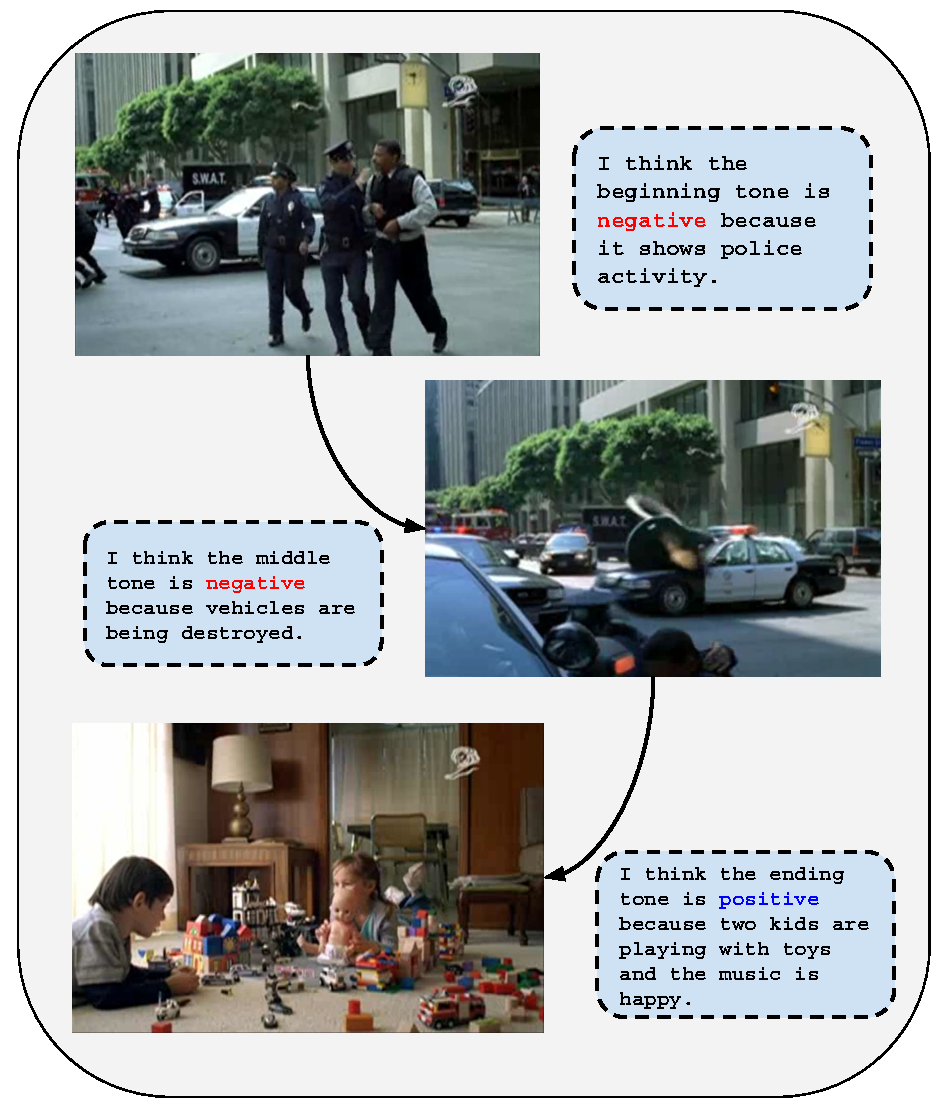
\includegraphics[width=0.5\columnwidth]{figures/Annotation_examples_tone_transition_new.pdf}
    \caption{Example provided to the annotators showing the tone transition and associated explanations}
    \label{tone_transition}
\end{figure}
\\
\textbf{\underline{Social message detection:}} For social message detection, the annotators are instructed to check for the absence/presence of social messages in the given video. Based on the social message framing in ads \cite{Brooks2020ExploringAO}, we provide the following definition to guide the annotation process:
\begin{itemize}
    \item An advertisement video has a social message if it provides awareness about any social issue. Examples include \textit{gender equality}, \textit{drug abuse}, \textit{police brutality}, \textit{workplace harassment}, \textit{domestic violence}, \textit{child labor}, \textit{homelessness}, \textit{hate crimes} etc.
\end{itemize}
To simplify the annotation process, we ask the annotators to mark Yes/No for indicating the presence/absence of social messages in the videos instead of marking the exact categories in the curated list of social issues \cite{ciment2006social}. The outline of the framework provided to annotators for marking the presence/absence of social messages is shown in Fig \ref{annot_framework}.
Further, annotators are also provided with example videos showing different forms of social messages. In Fig \ref{social_message} (a), frame transitions are shown from an example video urging everyone to vote since voters having bias can cast votes in their absence. In Fig  \ref{social_message} (b), sample frames in the sequence are shown from another example video highlighting the importance of equal opportunities for everyone in sports.
\begin{figure*}[h!]
\centering
    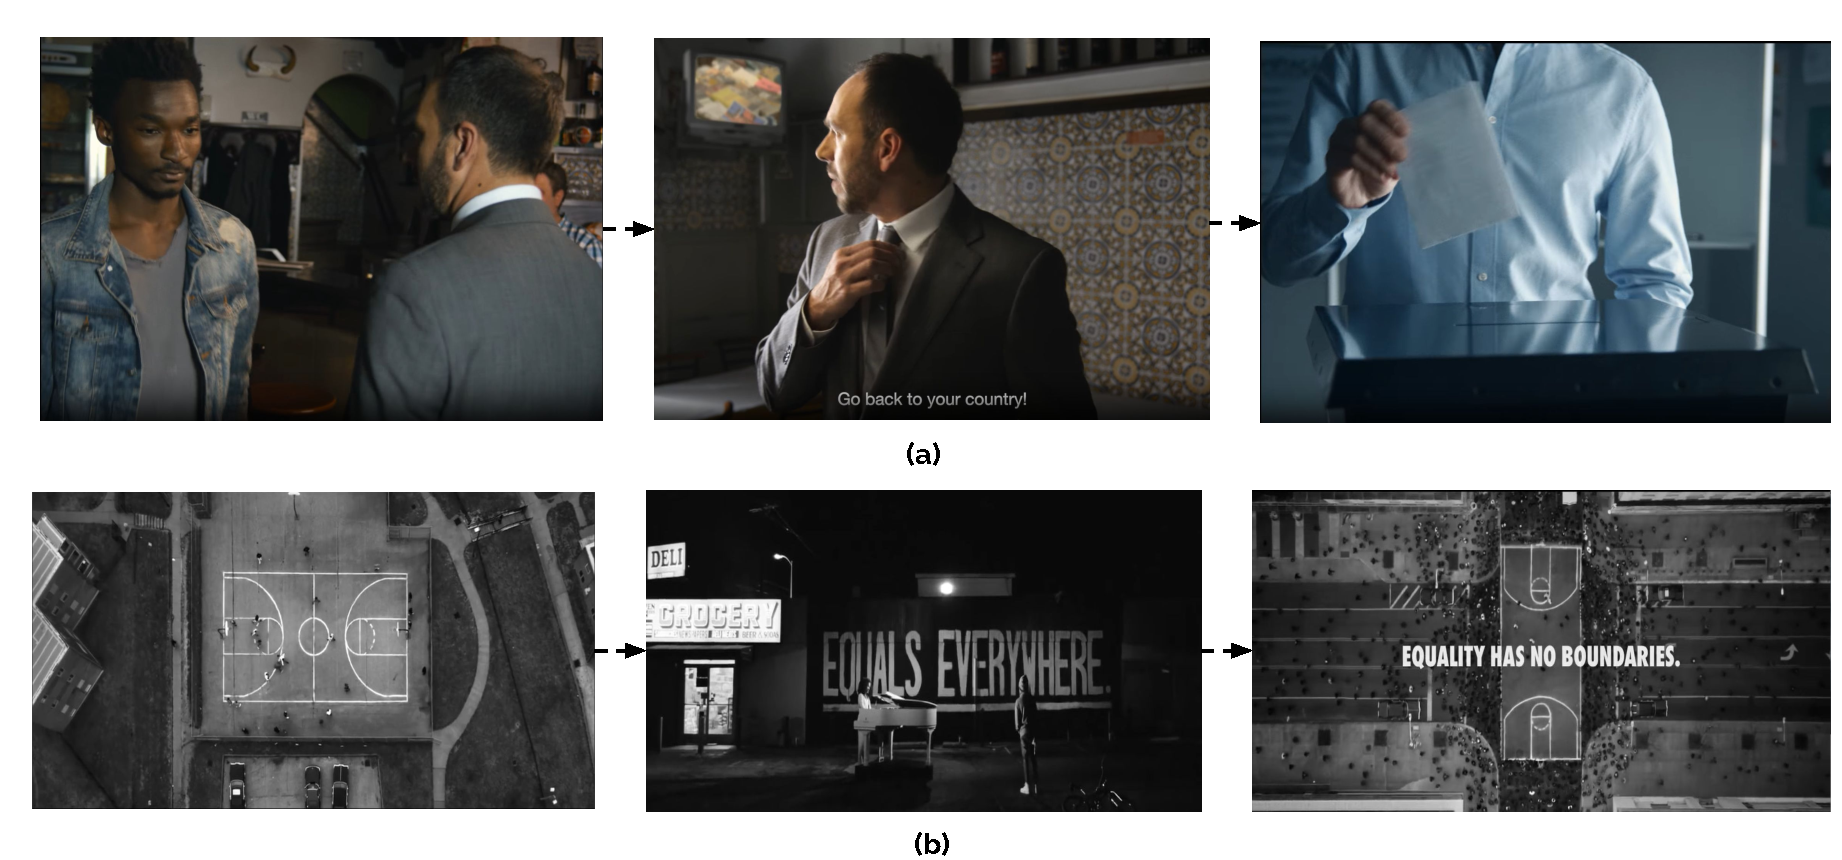
\includegraphics[width=0.8\textwidth]{figures/new_social_message_image.pdf}
    \caption{Example videos associated with absence/presence of social message provided to the annotators. (a) Frame transition associated with an example video urging people to vote (b) Frame transition associated with an example video emphasizing equal opportunities for everyone in sports.}
    \label{social_message}
\end{figure*}
\\
\textbf{\underline{Topic categorization:}}
We annotate topic categories using the existing taxonomies from Ads-of-the-world (AOW), Cannes Lions Film Festival \cite{cannes-lions}, and Video-Ads \cite{Hussain2017AutomaticUO} datasets. We denote the taxonomies associated with Cannes Lions Film Festival and Video-Ads datasets as Cannes-coding [\textcolor{purple}{\textbf{CC}}] and Video-Ads [\textcolor{blue}{\textbf{VA}}] coding schemes. 
We extract the available tags associated with 6304 videos in Ads-of-the-world [\textcolor{red}{\textbf{AOW}}] and retain the top 40 tags based on frequency. Then we manually merge the filtered topic tags from AOW with similar labels in Cannes-coding  [\textcolor{purple}{\textbf{CC}}] and Video-Ads [\textcolor{blue}{\textbf{VA}}] coding schemes. Some examples of merged labels from different sources are listed as follows with the final parent topic category:
\begin{itemize}
    \item \textbf{Publications media:} Media \& Publications  [\textcolor{purple}{\textbf{CC}}]; Media and arts [\textcolor{blue}{\textbf{VA}}]; TV Promos, Music, Media, Movies [\textcolor{red}{\textbf{AOW}}]
    \item \textbf{Games:} Games and toys [\textcolor{blue}{\textbf{VA}}]; Gaming [\textcolor{red}{\textbf{AOW}}]
    \item \textbf{Sports:} Sports equipment and activities [\textcolor{blue}{\textbf{VA}}]; Sports [\textcolor{red}{\textbf{AOW}}]
    \item \textbf{Clothing:} Clothing, Footwear \& Accessories [\textcolor{purple}{\textbf{CC}}]; Clothing and accessories [\textcolor{blue}{\textbf{VA}}]; Personal Accessories [\textcolor{red}{\textbf{AOW}}]
\end{itemize}
A detailed list of mapping between the AOW, CC and VA coding schemes is included as part of the Appendix (\ref{app:topic_categories}). Our final merged topic taxonomy consists of 18 categories as follows:
\begin{itemize}
    \item \textit{Games, Household, Services, Misc, Sports, Banking, Clothing, Industrial and agriculture, Leisure, Publications media, Health, Car, Electronics, Cosmetics, Food and Drink, Awareness, Travel and transport, Retail}
\end{itemize}
\textbf{\underline{Dataset Filtering:}} During the annotation process, we employ certain checks to maintain the quality of the annotated data. We reject those tone transition annotations with very short explanations (single words) or long generic descriptions of ads copied from the internet. Further, we also flag tone-transition annotations with the copied content across the start, middle, and end segments. For topic categorization, we merge categories with low frequencies, i.e., Alcohol and Restaurant, into the broad category of Food and Drink.
\subsection{Statistics}
MM-AU consists of 8399 annotated videos with a total of 147 hours of curated data. A detailed overview of MM-AU with total duration, number of tags, and year coverage is shown in Table \ref{Data_stats_table}.
\begin{table}[h!]
\centering
\begin{tabular}{@{}cc@{}}
\toprule
\textbf{Attribute} & \textbf{Value} \\ \midrule
\textbf{\#videos}           & 8399           \\
\textbf{\#explanations}     & 74970         \\
\textbf{\#topics}           & 18          \\
\textbf{\#social msg labels}       & 25197          \\
\textbf{\#tone labels}           & 75,591         \\
\textbf{\#duration}         & 147.79 hrs     \\
\textbf{\#avg duration}     & 63.35s         \\
\textbf{year}               & 2006-2019      \\
\textbf{\#annotators}       & 36             \\ 
\textbf{\#countries}       & 99             \\ \bottomrule
\end{tabular}
\caption{Data statistics of MM-AU dataset. \#social msg labels: total number of labels }
\label{Data_stats_table}
\end{table}
\begin{figure}[h!]
    \centering
    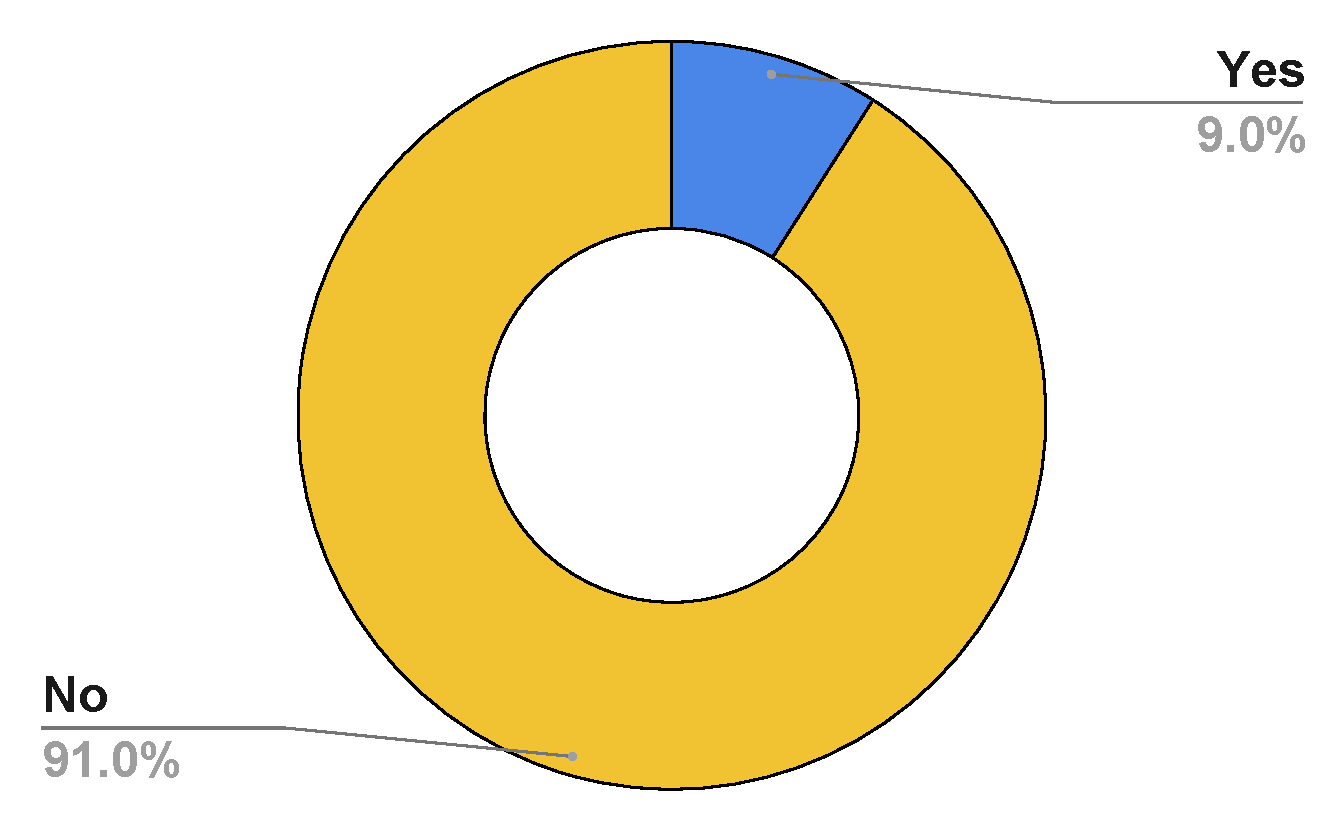
\includegraphics[width=0.6\columnwidth]{figures/social_message_majority.pdf}
    \caption{Distribution of the social message absence (No) and presence (Yes) labels in MM-AU}
    \label{Social_message_majority}
\end{figure}
\begin{figure*}[h!]
  \centering
  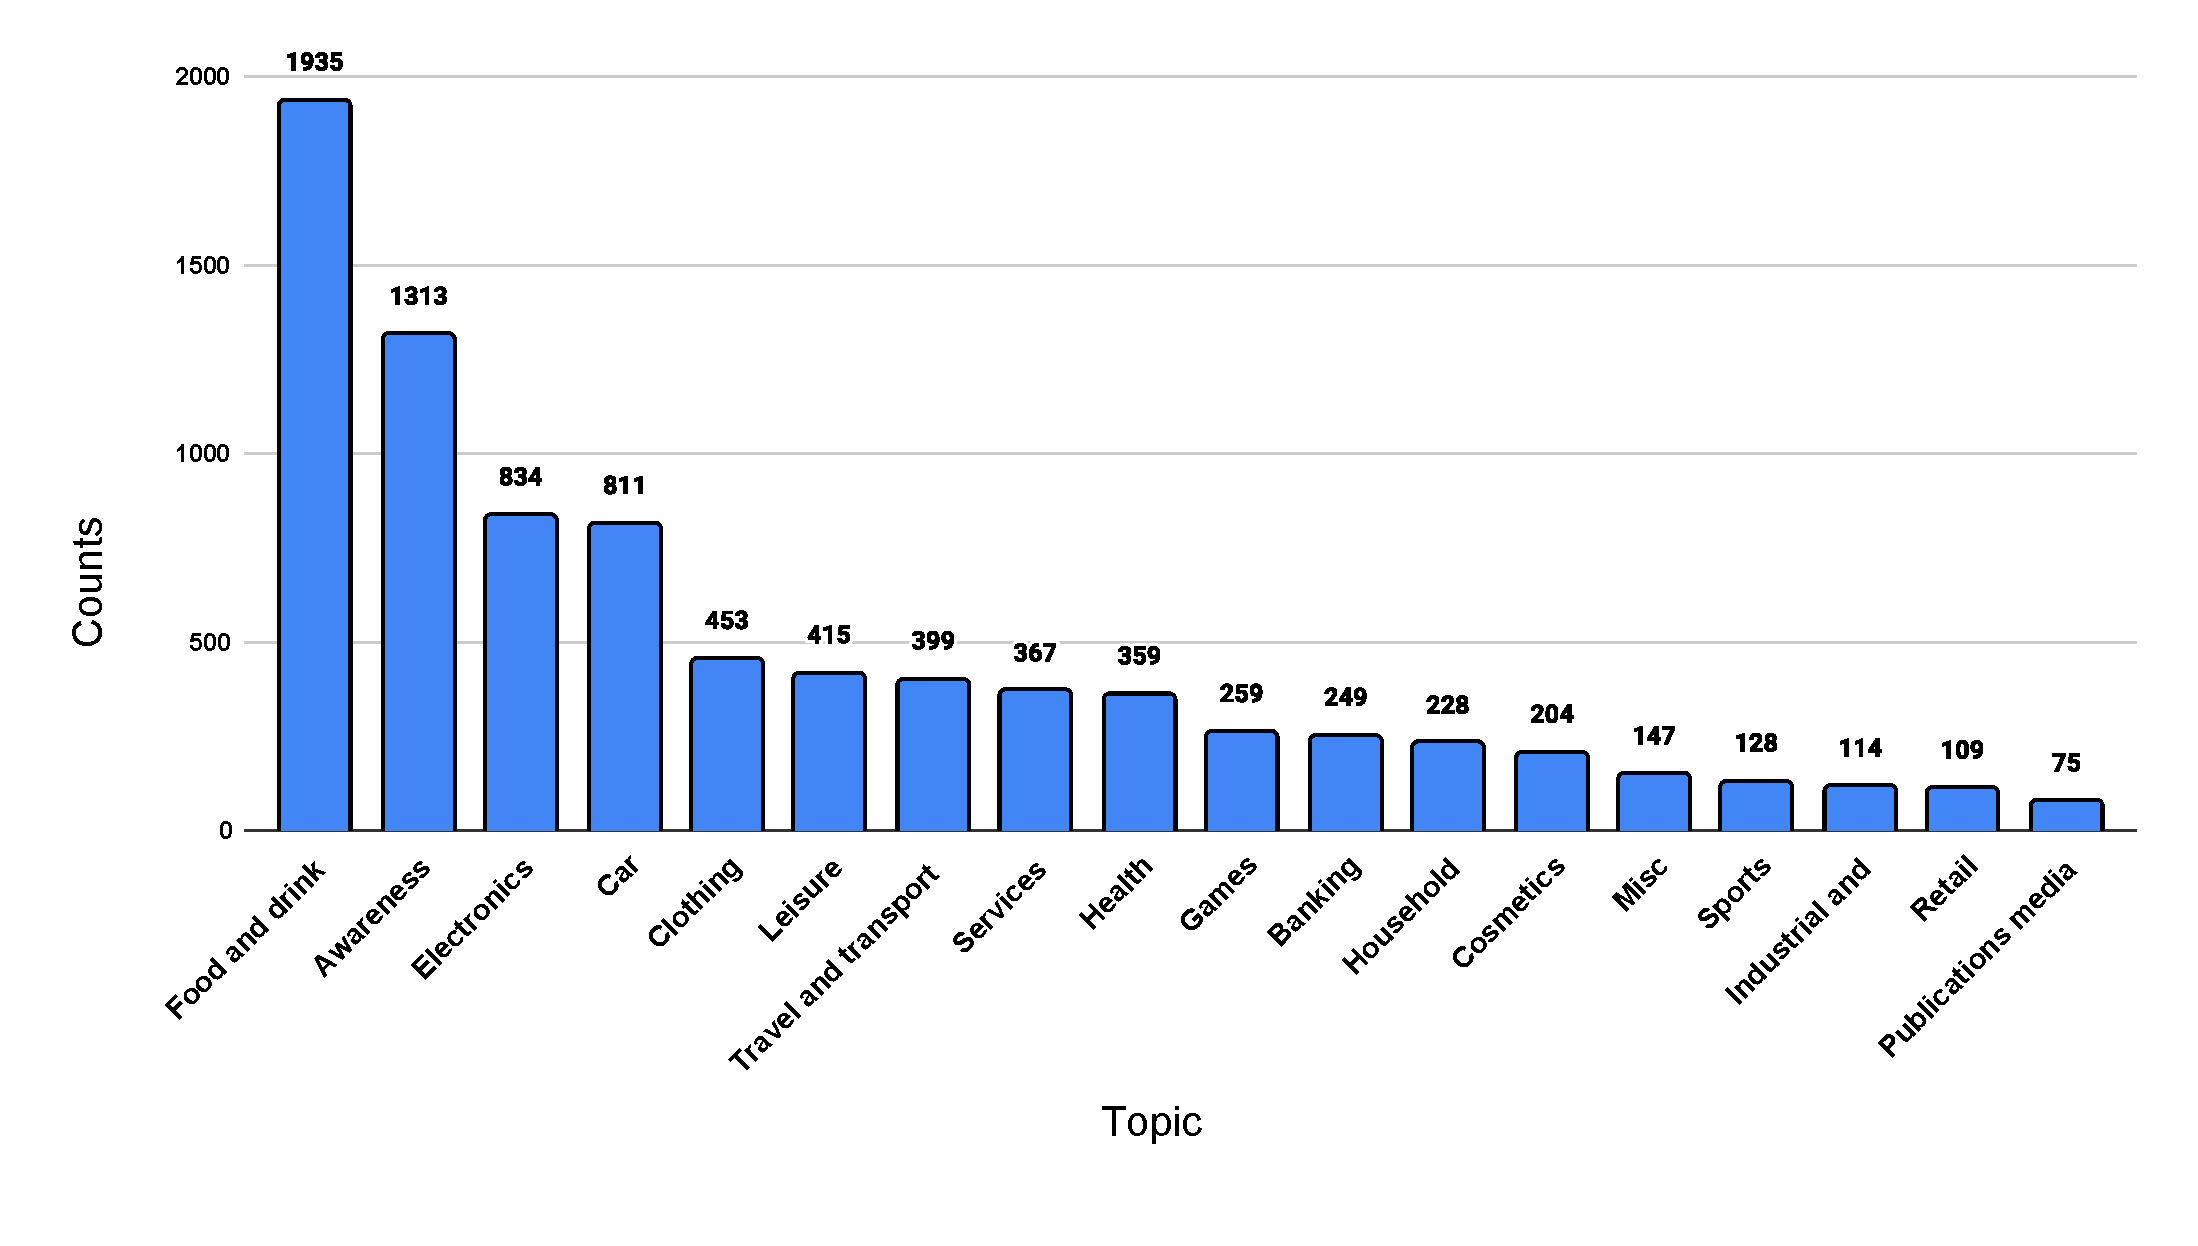
\includegraphics[width=\textwidth]{figures/topic_listing_new_pdf.pdf}
  \caption{Distribution of topics in MM-AU dataset}
  \label{topics}
\end{figure*}
The distribution of topics is shown in Fig~\ref{topics}, with Food and Drink, Awareness, and Electronics being the top-3 dominant categories. In the case of perceived tone labels, we obtain a high majority agreement among annotators in marking the start (\textbf{91.2\%}), middle (\textbf{91.6\%}), and the ending (\textbf{94.5\%}) segments of the videos with perceived tone labels. Since annotating the presence/absence of social messages is a comparatively less subjective task than perceived tone labeling, we obtain a majority agreement (\textbf{99\%}) among the annotators. In terms of tone labels for start, middle, and end segments, we can see from Fig~\ref{start_mid_end_tone}, that the dominant perceived tone for the advertisements is positive, with its share rising from \textbf{60.2\%} (start) to \textbf{81.3\%} (end). This can be explained due to the fact that advertisements are primarily designed to persuade viewers to buy certain products or act toward certain social issues. However, from Fig~\ref{start_mid_end_tone}, we can see that the share of negative tone labels increases from \textbf{15.5\%} to \textbf{19.6\%} due to the narrative structure of the ads, where the middle segment portrays negative elements like human suffering, environmental damage, etc to set up the final conclusion. From Fig~\ref{Social_message_majority}, we can see that \textbf{9.0\%} of the videos, i.e. 759 contain social messages, as marked by \textbf{Yes} label. Out of 759 videos, \textbf{62.5\%} exhibit transition in perceived tone with the share of negative tone rising from \textbf{32.3\%} to \textbf{43.3\%} in the middle segments.

% \begin{figure}[h!]
% \centering
% \subfloat[]{%
% 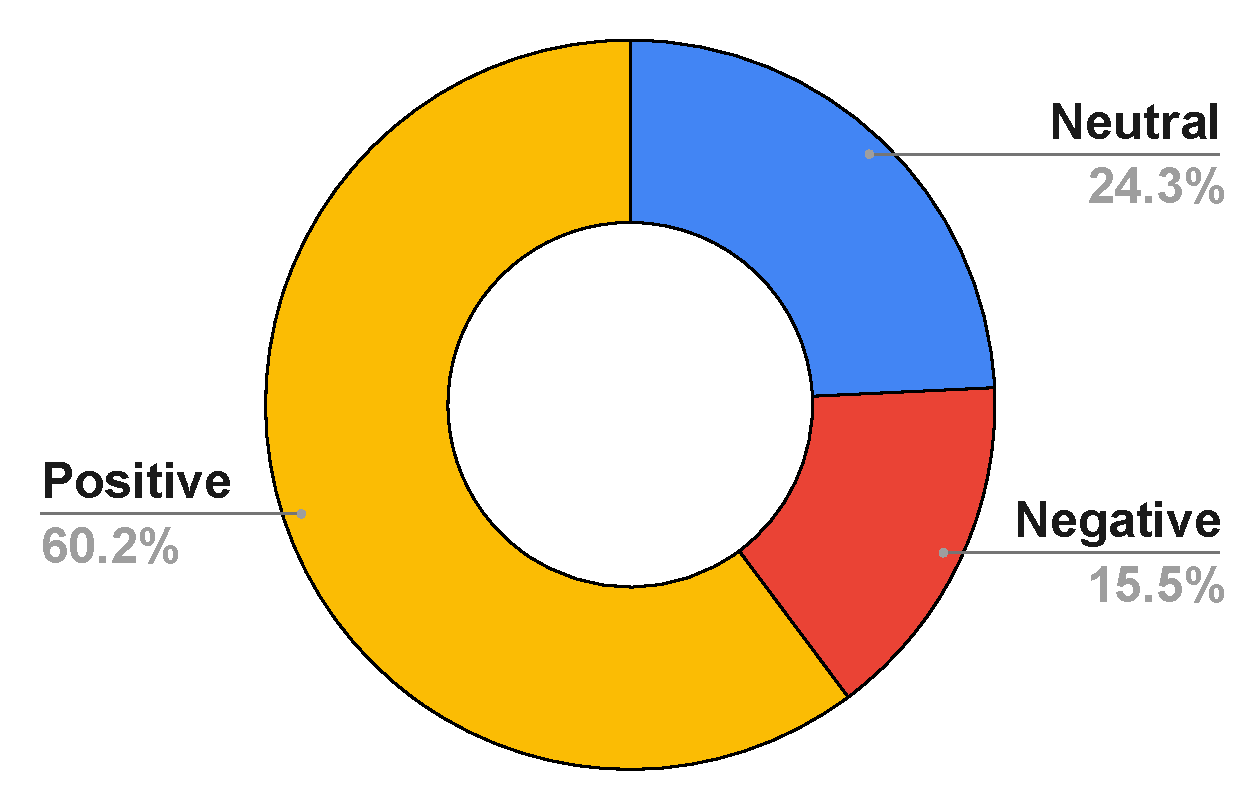
\includegraphics[width=0.33\textwidth]{figures/start_tone_majority.pdf}% 
% \label{start_tone}
% }
% \subfloat[]{%
% 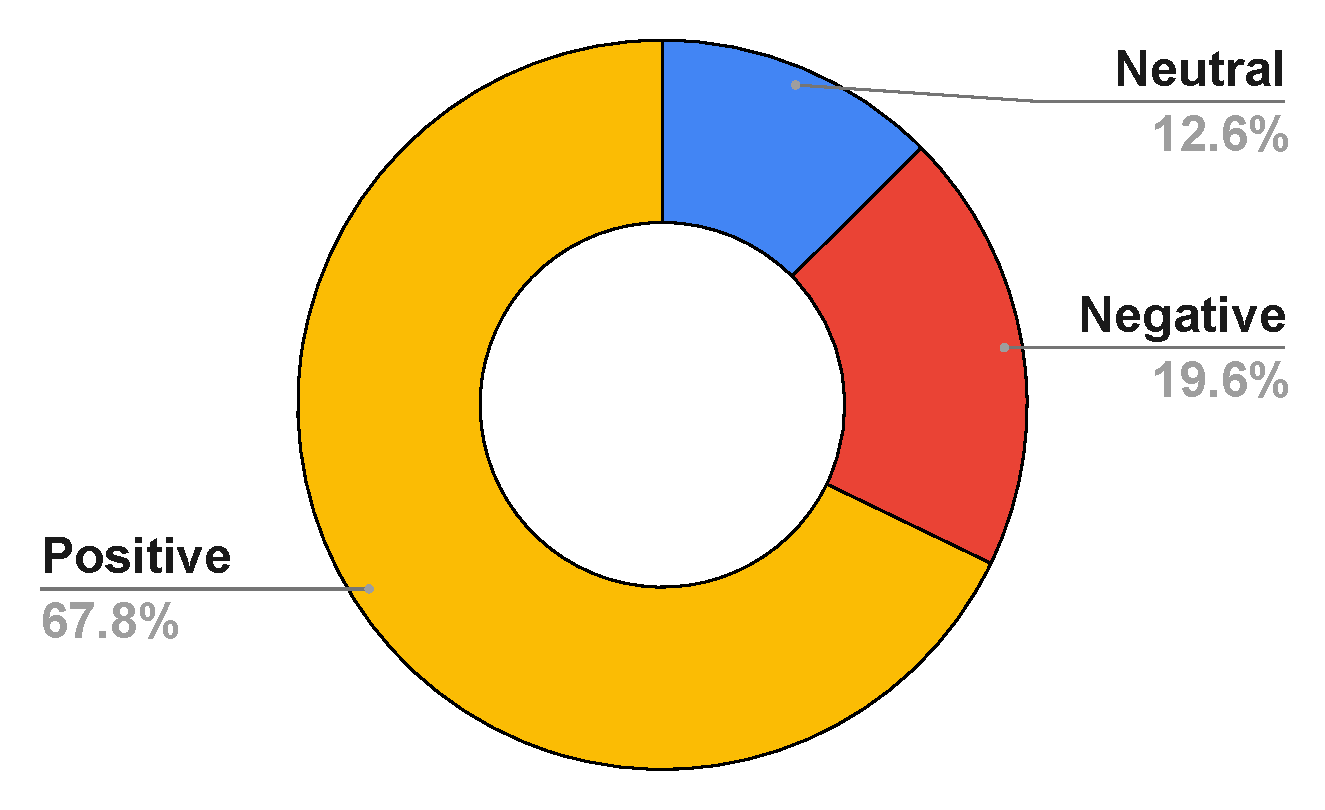
\includegraphics[width=0.33\textwidth]{figures/middle_tone_majority.pdf}%
% \label{mid_tone}
% }
% \subfloat[]{%
% 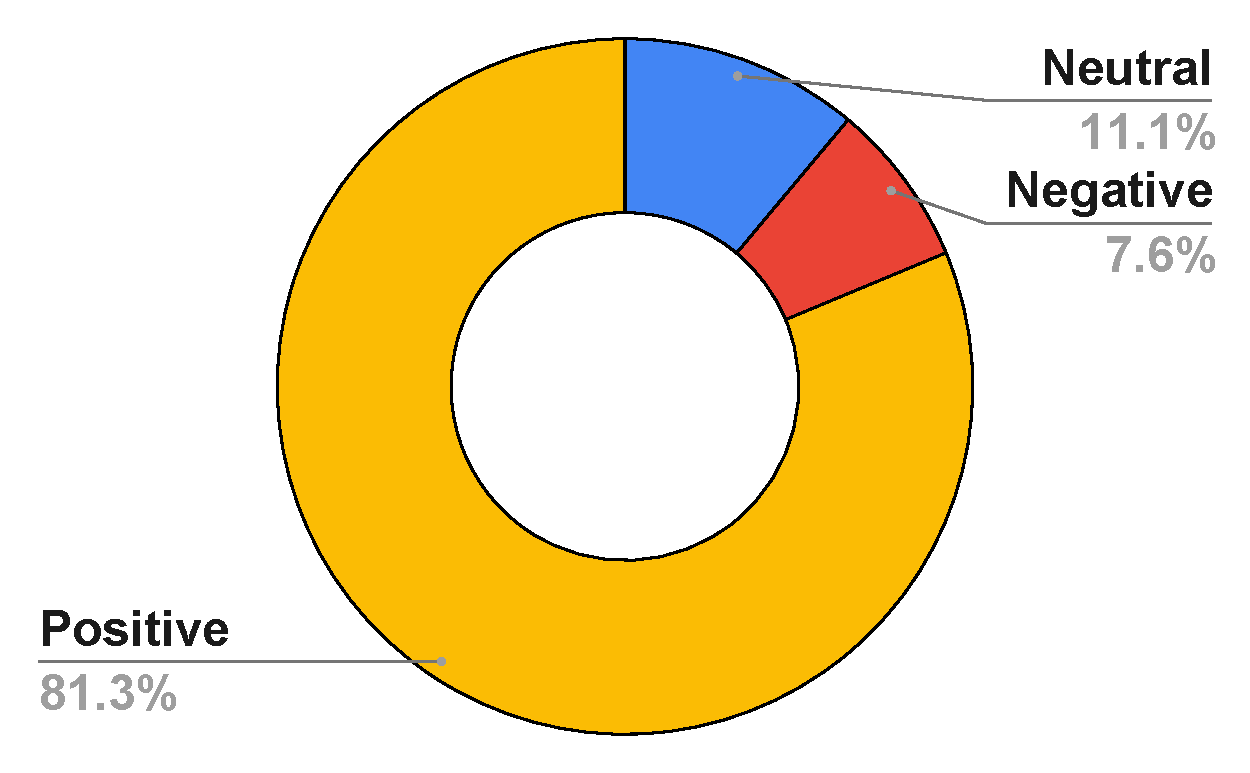
\includegraphics[width=0.34\textwidth]{figures/end_tone_majority.pdf}%
% \label{mid_tone}
% }
% \caption{Distribution of majority perceived tone labels (among 3 annotators) across (a) start, (b) middle, and (c) ending segments in MM-AU dataset (8399 videos) }
% \label{start_mid_end_tone}
% \end{figure}
\begin{figure}
\begin{subfigure}{.33\textwidth}
  \centering
  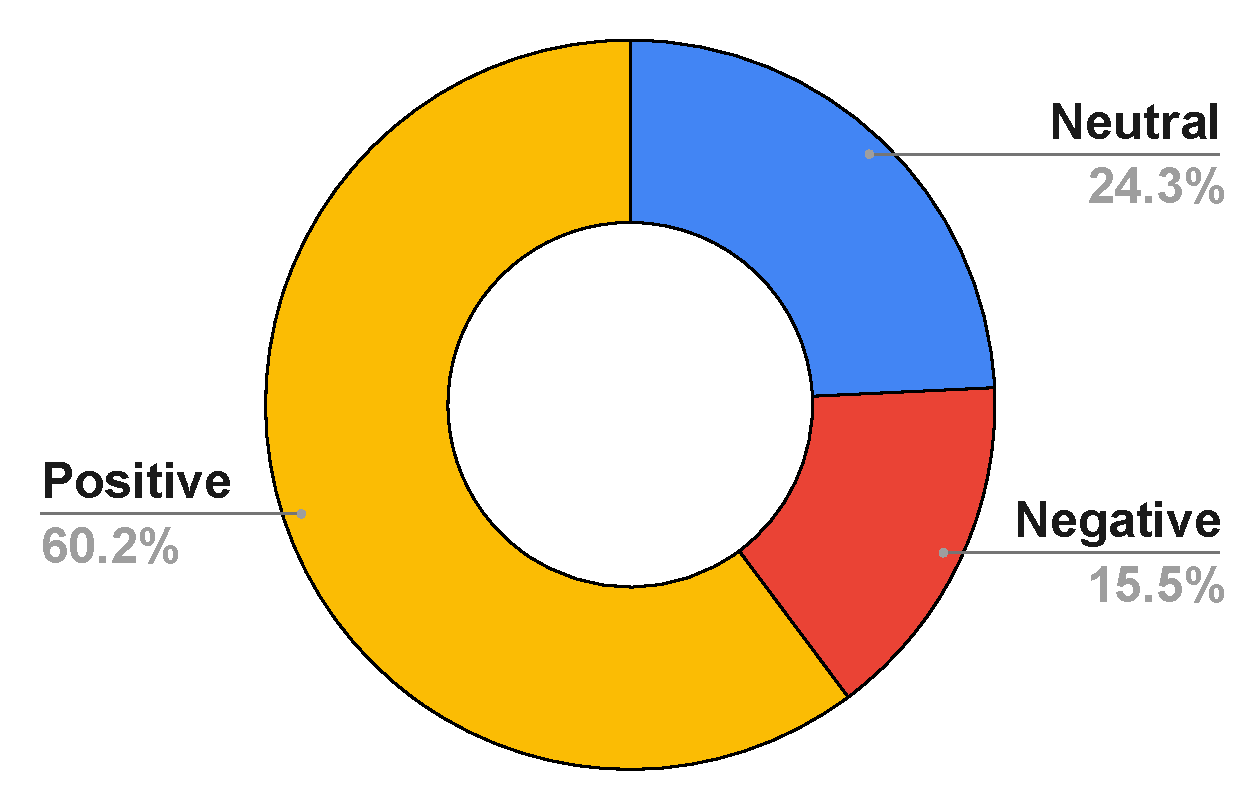
\includegraphics[width=.8\linewidth]{figures/start_tone_majority.pdf}
  \caption{Start segment}
  \label{start_tone}
\end{subfigure}%
\begin{subfigure}{.33\textwidth}
  \centering
  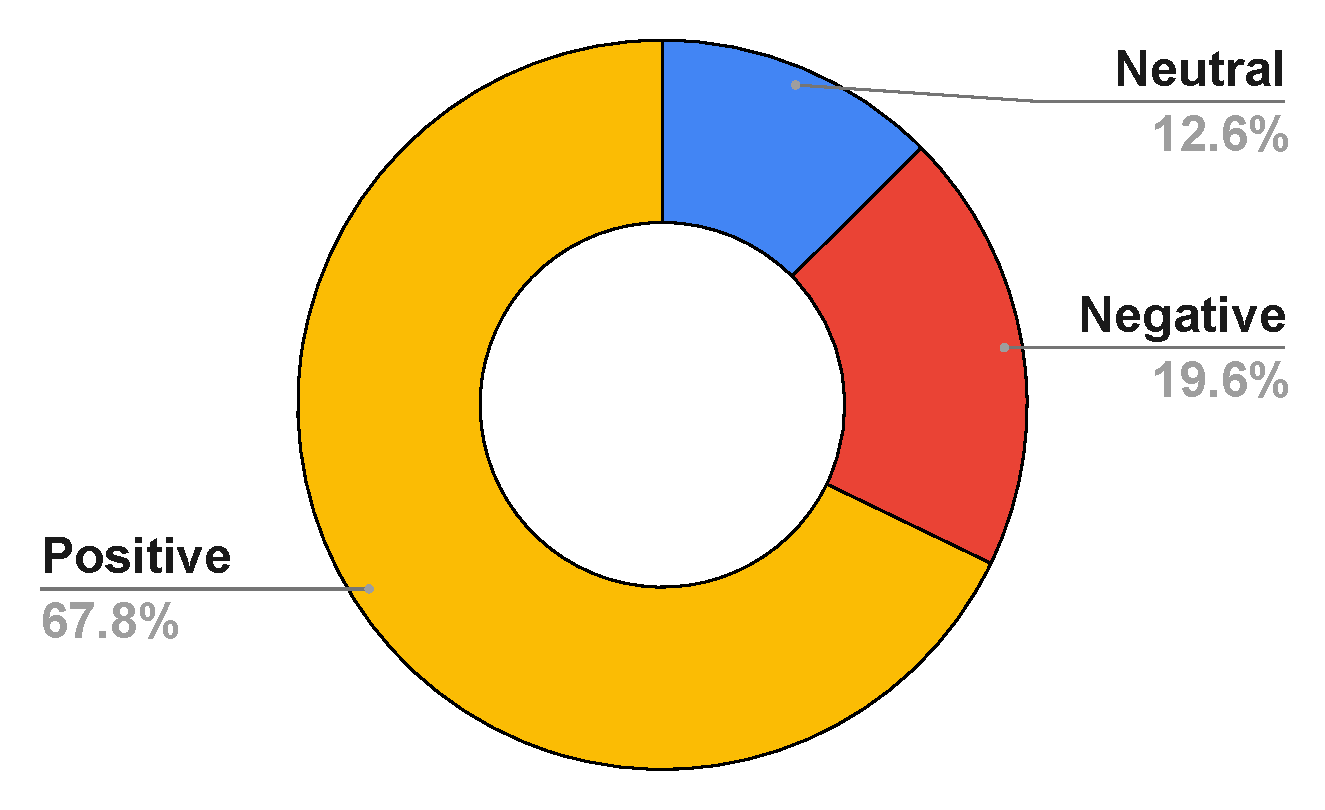
\includegraphics[width=.8\linewidth]{figures/middle_tone_majority.pdf}
  \caption{Middle segment}
  \label{mid_tone}
\end{subfigure}
\begin{subfigure}{.33\textwidth}
  \centering
  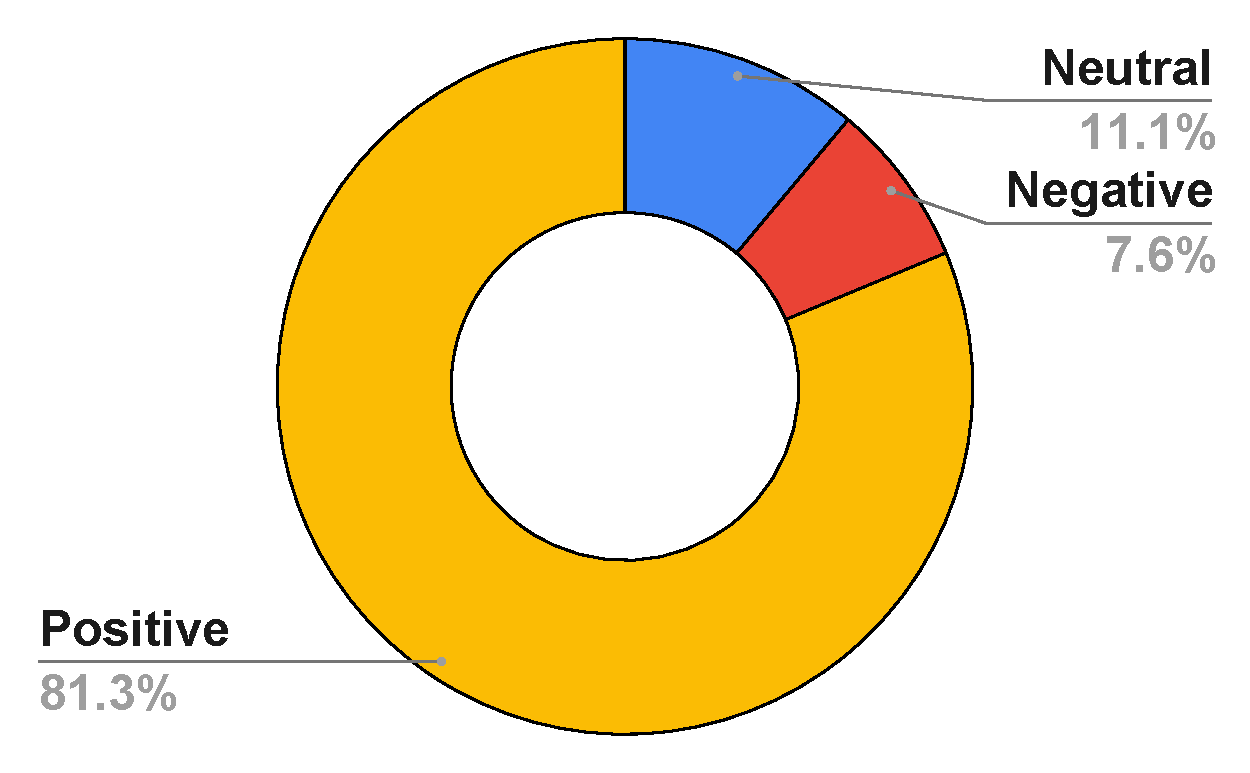
\includegraphics[width=.8\linewidth]{figures/end_tone_majority.pdf}
  \caption{End segment}
  \label{end_tone}
\end{subfigure}
\caption{Distribution of majority perceived tone labels (among 3 annotators) across (a) start, (b) middle, and (c) ending segments in MM-AU dataset (8399 videos) }
\label{start_mid_end_tone}
\end{figure}

\begin{figure}
\begin{subfigure}{.50\textwidth}
  \centering
  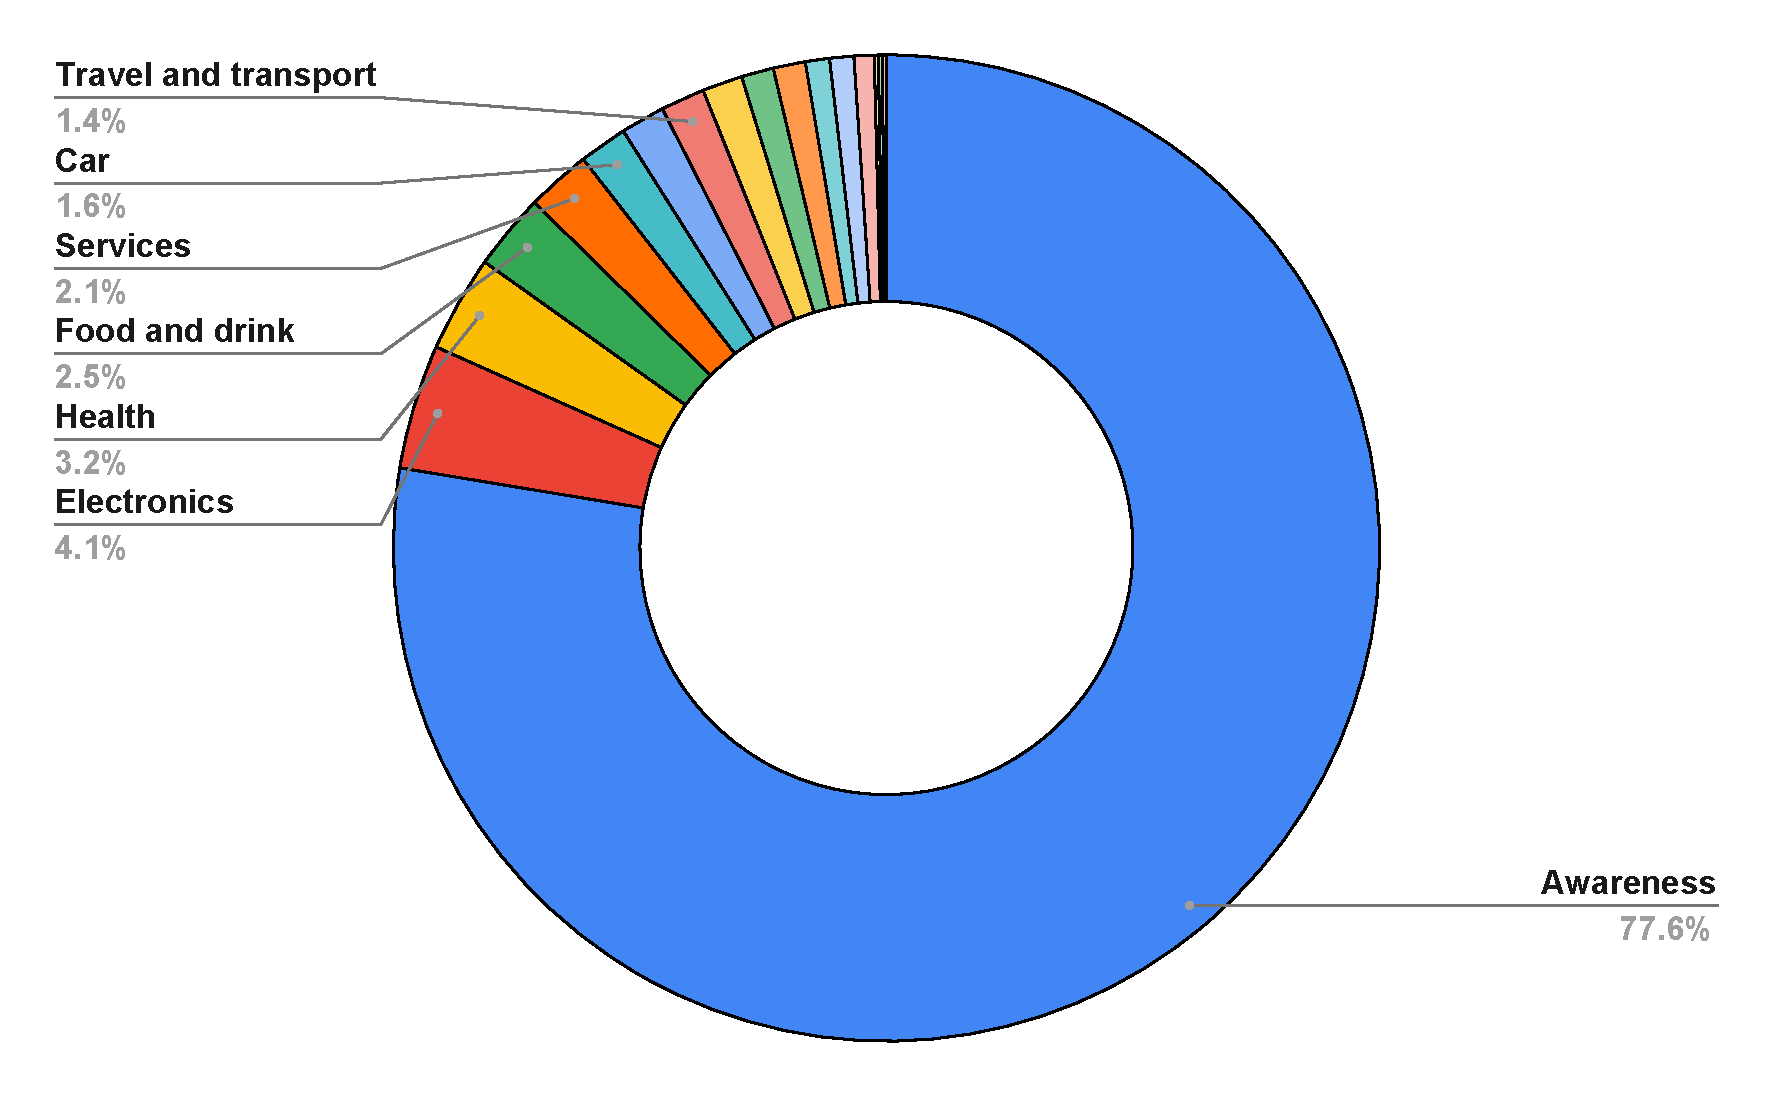
\includegraphics[width=\linewidth]{figures/topic_vs_social_message.pdf}
  \caption{Distribution of Topics wrt social message}
  \label{topic_social_message}
\end{subfigure}%
\begin{subfigure}{.50\textwidth}
  \centering
  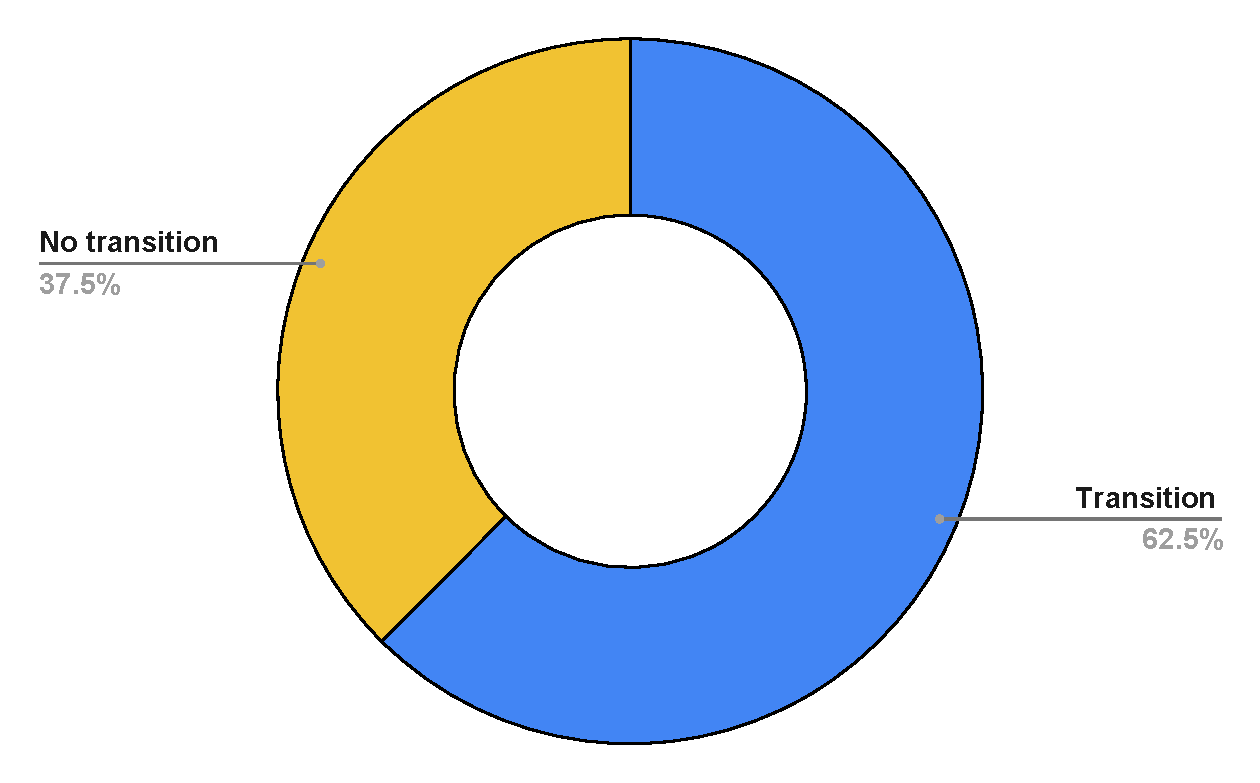
\includegraphics[width=\linewidth]{figures/transition_vs_social_message.pdf}
  \caption{Distribution of Tone transition wrt social message}
  \label{tone_transition_social_message}
\end{subfigure}
\caption{Distribution of topics and perceived tone transition across videos having the presence of social message (739 videos) in MM-AU dataset}
\label{topic_tone_transition_social_message}
\end{figure}
We further explore the intersection between the presence of social message and associated topics and tone transition (including tone labels for different segments of the video). From Fig \ref{topic_tone_transition_social_message} (a), we can see that out of 739 videos having social messages, \textbf{77.9\%} have \textbf{Awareness} as the associated topic label. The \textbf{Awareness} topic label includes subcategories related to social issues involving environmental damage, animal rights, smoking, alcohol abuse, domestic violence, refugee crisis, cyberbullying, etc. Further, as shown in Fig \ref{topic_tone_transition_social_message} (b), we observe a greater incidence of transitions in perceived tone (\textbf{62.5\%}) associated with videos having social messages. A detailed breakdown of segment-wise perceived tone labels for videos having social messages is shown in Fig \ref{start_mid_end_soc_msg_tone}. We can see an increase in the perceived negative tone from \textbf{32.3\%} to \textbf{43.3\%}. This can be attributed to the narrative structure of the advertisement videos having the presence of a social message where the middle segment primarily portrays negative elements i.e. environmental damage, human suffering etc to set up the conclusion.
\begin{figure}
\begin{subfigure}{.33\textwidth}
  \centering
  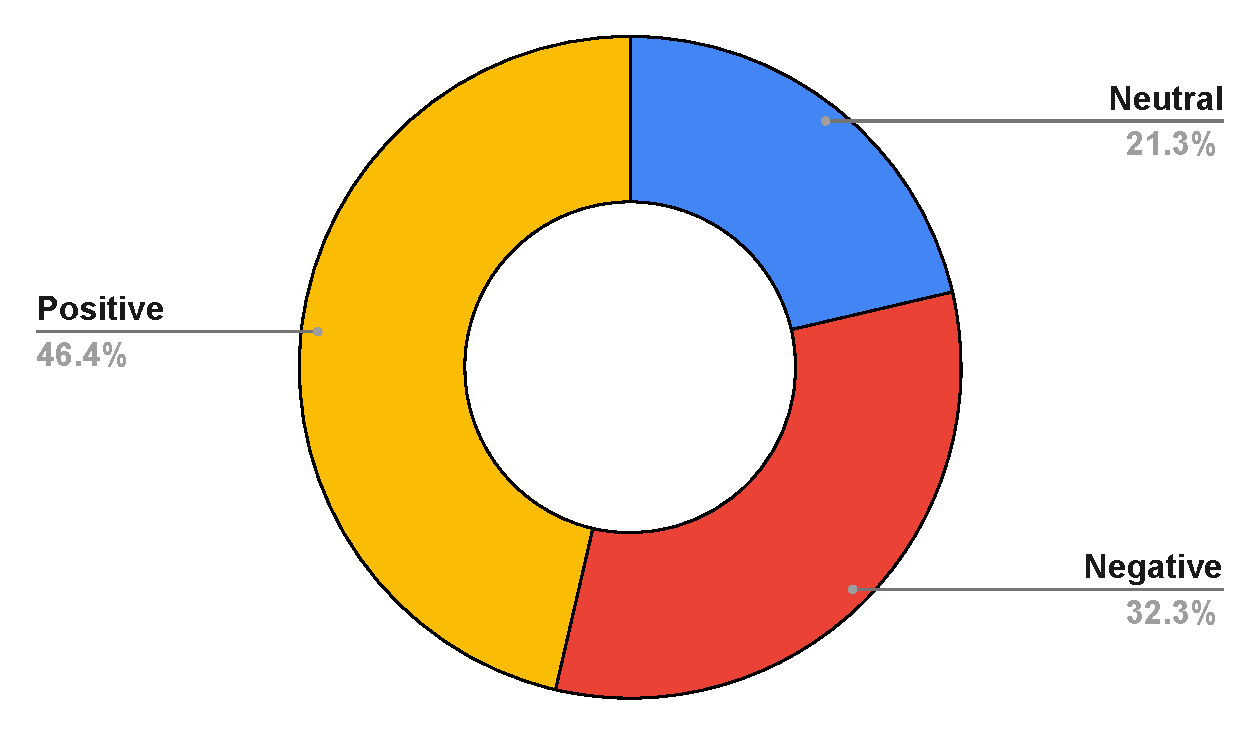
\includegraphics[width=\linewidth]{figures/start_tone_vs_social_message.pdf}
  \caption{Start segment}
  \label{start_tone_social_message}
\end{subfigure}%
\begin{subfigure}{.33\textwidth}
  \centering
  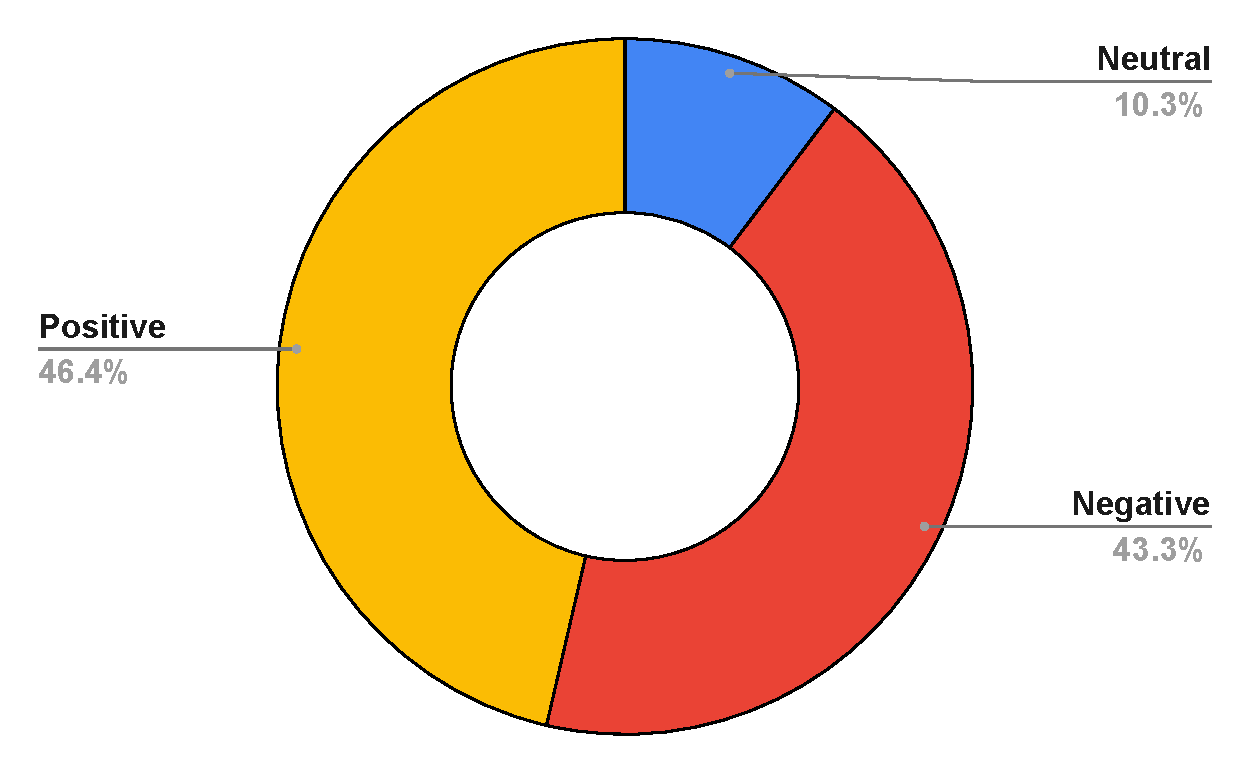
\includegraphics[width=\linewidth]{figures/middle_tone_vs_social_message.pdf}
  \caption{Middle segment}
  \label{mid_tone_social_message}
\end{subfigure}
\begin{subfigure}{.33\textwidth}
  \centering
  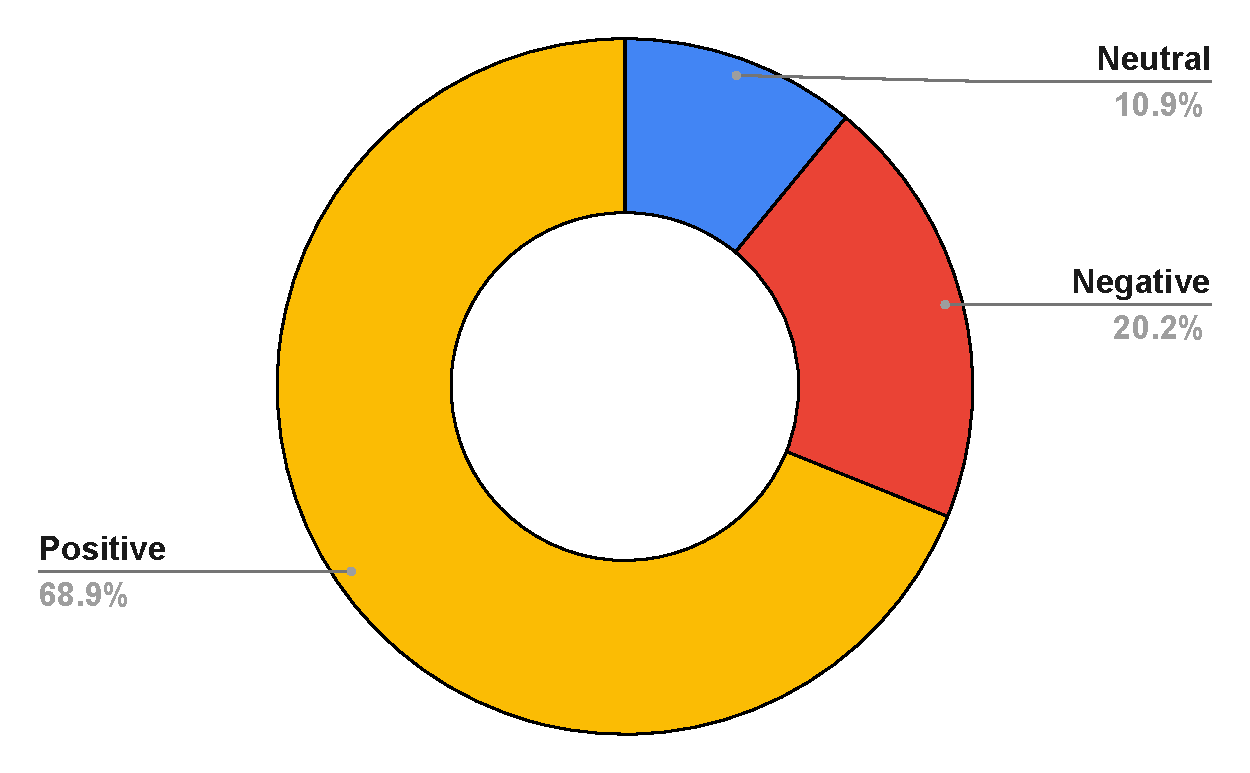
\includegraphics[width=\linewidth]{figures/ending_tone_vs_social_message.pdf}
  \caption{End segment}
  \label{end_tone_social_message}
\end{subfigure}
\caption{Distribution of perceived tone labels across the (a) start, (b) middle, and (c) ending segments in MM-AU dataset for videos having social message (739 videos) }
\label{start_mid_end_soc_msg_tone}
\end{figure}



\section{Task definition}
\textbf{\underline{Social message detection:}}
Based on the social message annotations (majority), the presence/absence of social message (SM) for $ith$ video is defined as:
\begin{equation}
  SM_{i} =
    \begin{cases}
      0 & \text{No (Absence of SM)}\\
      1 & \text{Yes (Presence of SM)}
    \end{cases}       
\end{equation}
Our aim is to learn a network $f_{SM}$ to predict social message presence/absence $\hat{SM}_{i}$ for the $ith$ video. The above definition results in 759 and 7640 videos marked with the presence  (1) and absence (0) of social messages, respectively.\\
\textbf{\underline{Tone transition:}}
Based on the start, middle, and end perceived tone labels (majority), we define the transition for $ith$ video as follows:
\begin{equation}
  Tr_{i} =
    \begin{cases}
      0 & \text{$Start_{i}=Mid_{i}=End_{i}$}\\
      1 & \text{else}
    \end{cases}       
\end{equation}
Our aim is to learn a multimodal network $f_{Tr}$ to predict binary tone transition $\hat{Tr}_{i}$ for the $ith$ video.
MM-AU dataset has 3854 and 4545 videos marked with Transition (1) and No Transition (0), respectively.\\
\textbf{\underline{Topic categorization:}}
For topic categorization, we aim to learn a multimodal network $f_{Topic}$ to predict $\hat{Topic}_{i}$ for the $ith$ video out of 18 target categories. 
\section{Context through multimodality}
In the case of advertisements, we utilize the available information with temporal and foreground contexts for macro-level understanding based on the previously mentioned tasks of topic categorization, social message detection, and tone transition. The context information can be processed through the modalities mentioned below:
\begin{itemize}
    \item \textbf{Temporal context:} Visual modality (shots with different camera viewpoints and semantic divisions), Audio modality 
      (Background music and audio events).
    \item \textbf{Foreground context:} Language modality (Narrations/descriptions through text transcripts).
\end{itemize}

\section{Multimodal context fusion}
\begin{figure}[h!]
     \centering
     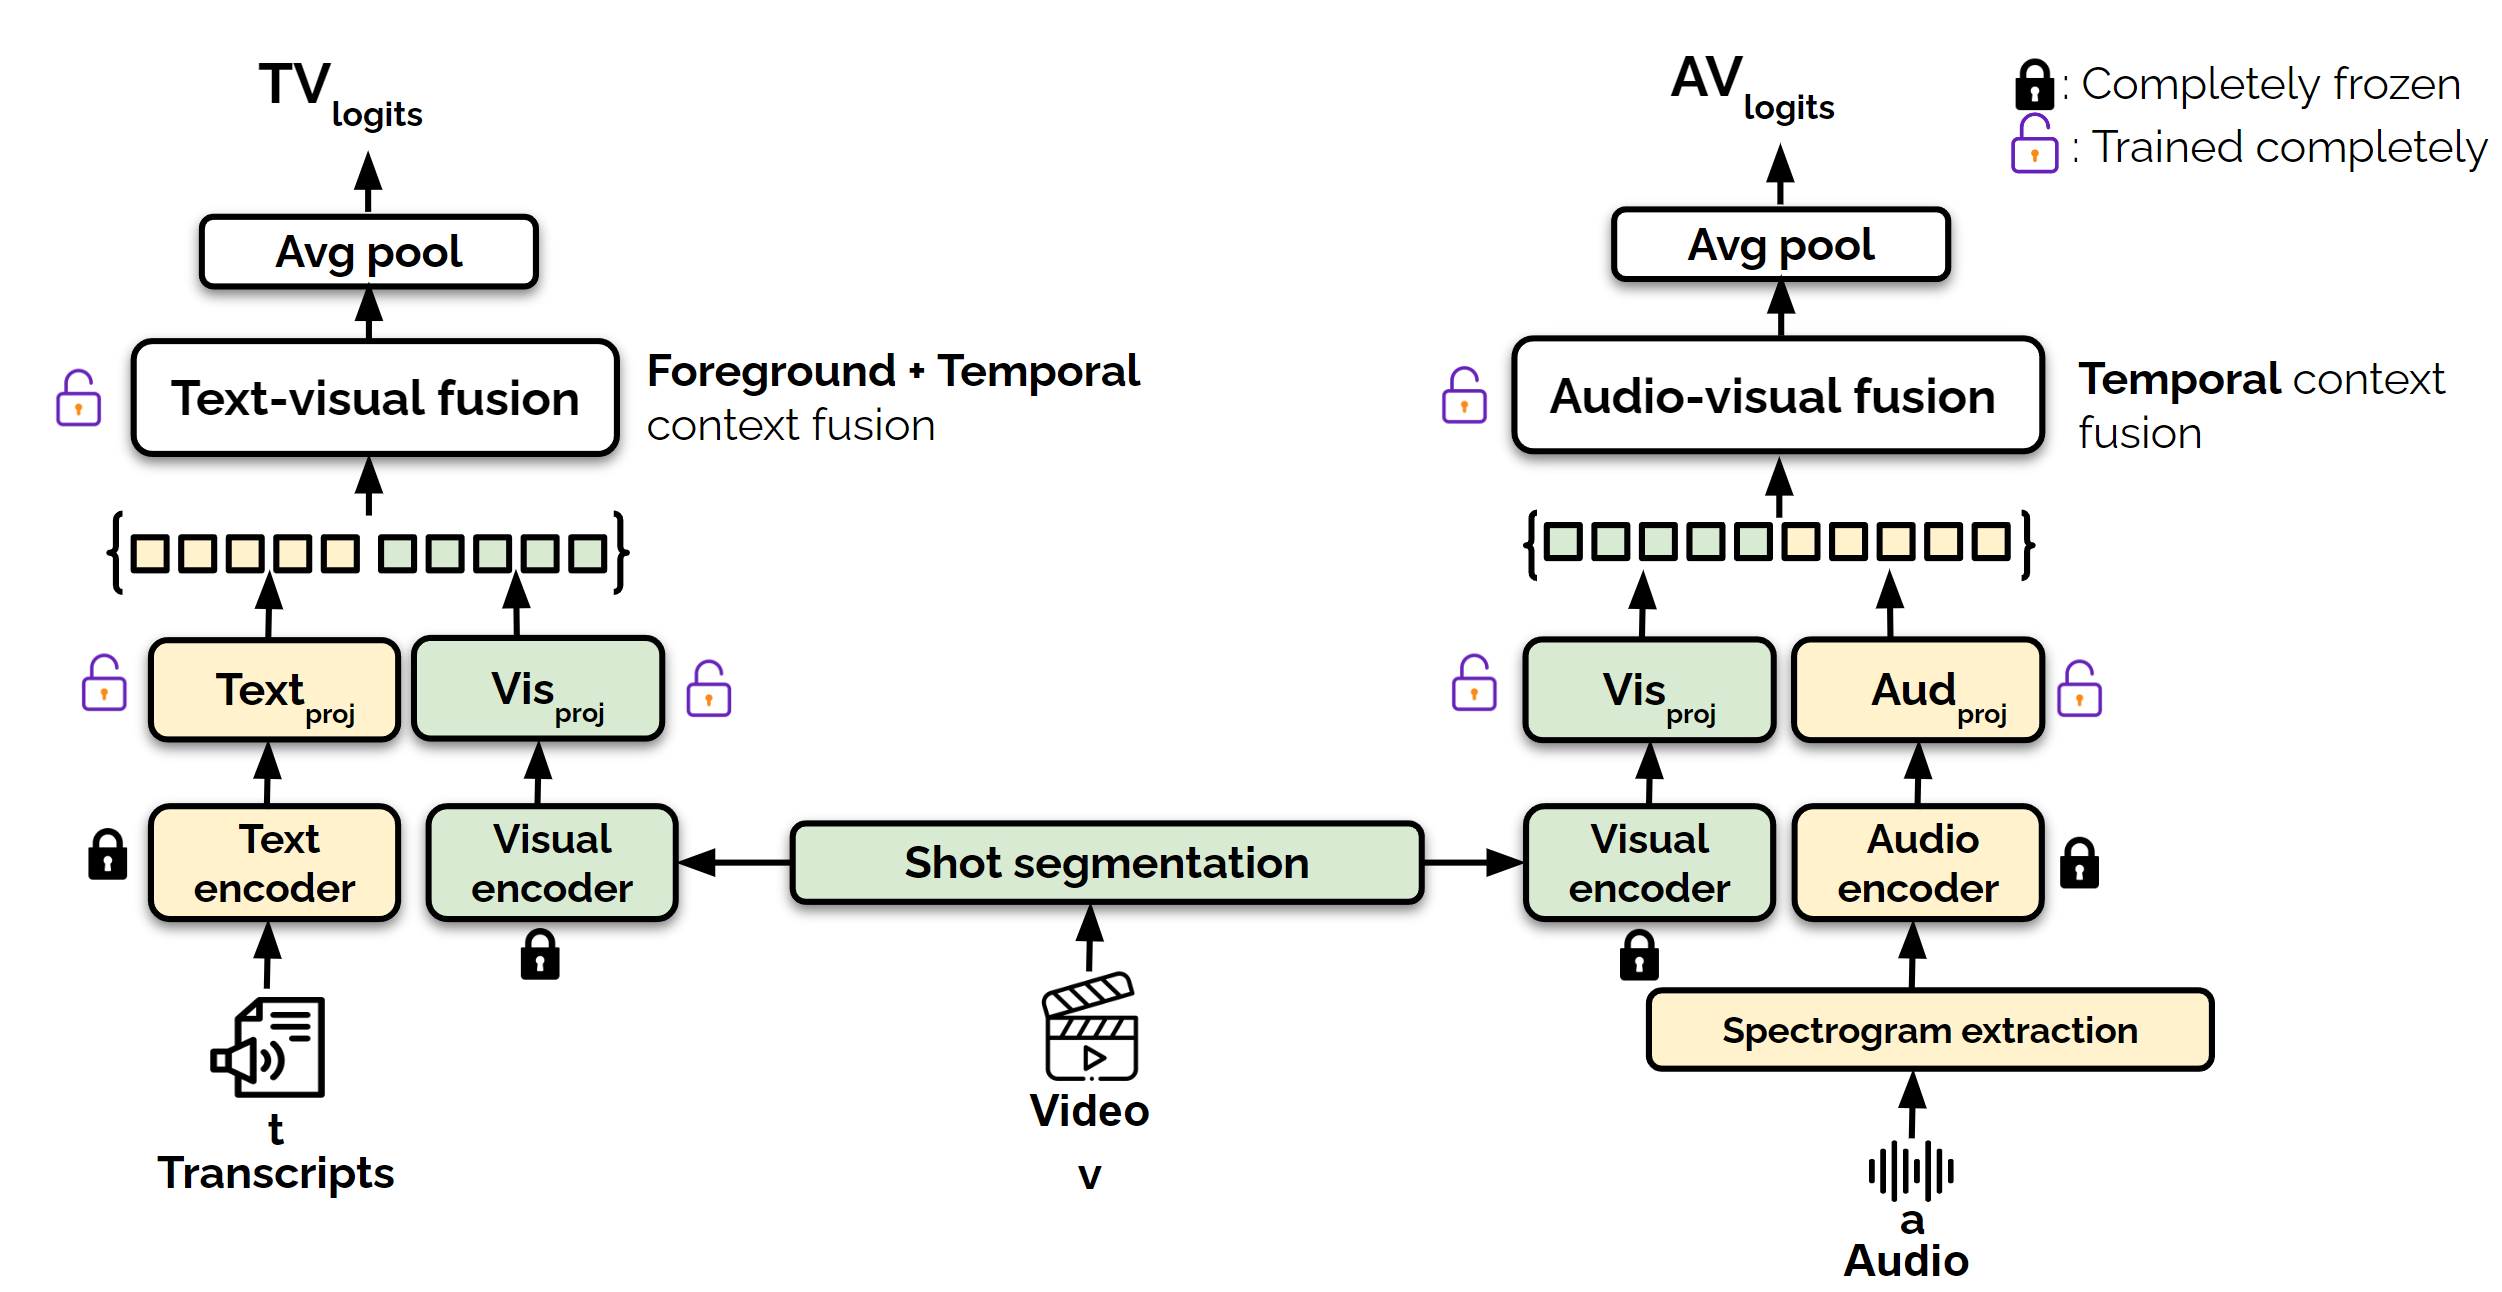
\includegraphics[width=\textwidth]{figures/ads_modeling_structure.png}
    \caption{Proposed architecture for the fusion of different modalities associated with temporal and foreground contexts. }
\end{figure}
For the input modalities $a$, $v$, $t$, we outline the separate context-guided fusion operations as follows:
\subsection{Foreground and temporal context fusion}
We outline the operations for foreground (\textbf{language}) and temporal (\textbf{visual}) context fusion as follows:
 \begin{align}
    \begin{split}
     e_{text}&=Text_{proj}(f_{text}(t))\\
     e_{vis}&=Vis_{proj}(f_{visual}(v)) \\ 
     TV_{logits}&=\mathbf{AvgPool}(\mathbf{{Tx}_{TV}}([e_{text};e_{vis}])) \\
    \end{split}
 \end{align}
 Here, $\mathbf{{Tx}_{TV}}$ is the text-visual fusion block used for combining foreground (\textbf{text}) and temporal (\textbf{visual}) contexts. $f_{visual}$ and $f_{text}$ refer to the pretrained visual and text encoders. The linear projection layers for visual and text modalities are denoted by $Vis_{proj}$ and $Text_{proj}$. 

\subsection{Temporal context fusion}
For the temporal context fusion block we have the following sequence of operations:
\begin{align}
    \begin{split}
     e_{aud}&=Aud_{proj}(f_{aud}(a))\\
     e_{vis}&=Vis_{proj}(f_{visual}(v)) \\ 
     AV_{logits}&=\mathbf{AvgPool}(\mathbf{{Tx}_{AV}}([e_{aud};e_{vis}])) \\
    \end{split}
\end{align}
 Here, $\mathbf{{Tx}_{AV}}$ is the audio-visual fusion block used for combining temporal context information from (\textbf{audio}) and   (\textbf{visual}) modalities. $f_{visual}$ and $f_{aud}$ refer to the pretrained visual and audio encoders. The linear projection layers for visual and audio modalities are denoted by $Vis_{proj}$ and $Aud_{proj}$. 

 For the fusion blocks, we consider the PerceiverIO transformer architecture \cite{Jaegle2021PerceiverIA} due to the following reasons:

 \begin{itemize}
    \item \textbf{Reduction in operational complexity:} In the case of PerceiverIO, the input embedding matrix having a significantly large sequence length is mapped to a limited group of latent vectors followed by attention operation on the latent vectors. This decreases the operational complexity of the attention operation. In Fig \ref{Perceiver}, $N$ is smaller than input sequence length $M$.
    \item \textbf{Generalization to a wide variety of inputs:} PerceiverIO architecture has been shown to be highly generalizable to a wide variety of inputs, including video, audio, and point clouds.
 \end{itemize}

In our proposed approach, we train the fusion blocks $\mathbf{{Tx}_{AV}}$ and $\mathbf{{Tx}_{TV}}$ separately due to overfitting issues faced while using a single fusion block for three modalities. Further, the combinations of different modalities (\textbf{audio-visual}) and (\textbf{text-visual}) contain complementary information that further improves macro-level understanding across the tasks in MM-AU benchmark. In order to capture the complementary information, we perform logit fusion by freezing the $\mathbf{{Tx}_{AV}}$ and $\mathbf{{Tx}_{TV}}$ blocks using the following strategies:

\begin{itemize}
    \item \textbf{A-max:} $pred_{class}=\argmaxA_i (TV_{logits}(i)+AV_{logits}(i))/2$
    \item \textbf{D-max:} $pred_{class}=\argmaxA_i max\{(TV_{logits}(i),AV_{logits}(i))\}$
\end{itemize}
Here $i \in \{1,...Class\}$, where $Class$ refers to the number of classes associated with the task.

 \begin{figure}
 \centering
    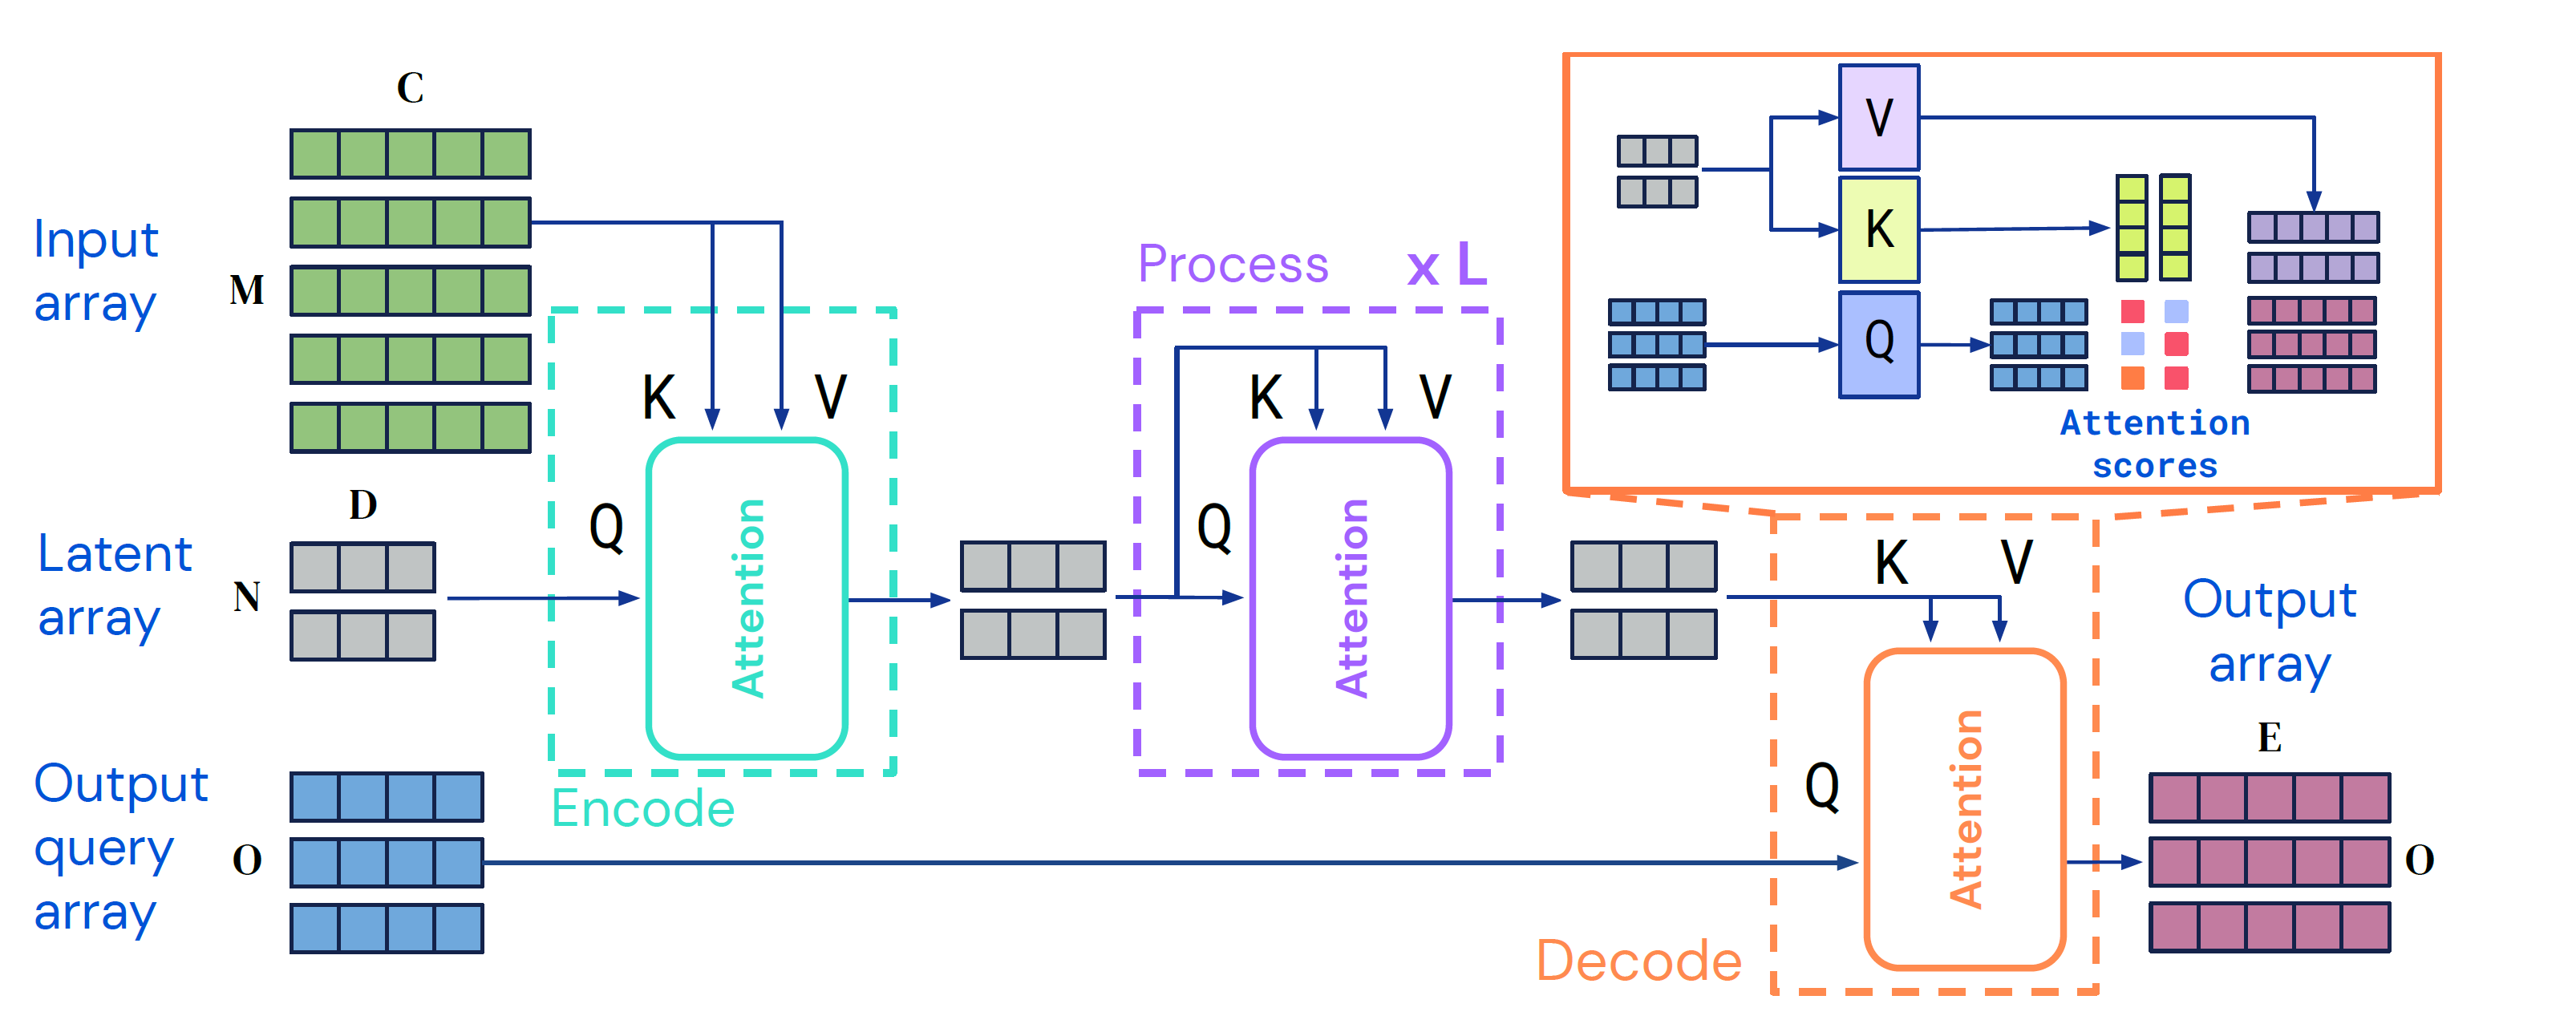
\includegraphics[width=0.8\textwidth]{figures/perceiver_architecture.png}
    \caption{PerceiverIO architecture \cite{Jaegle2021PerceiverIA}}
    \label{Perceiver}
 \end{figure}

\section{Experiments}
\subsection{Experimental Setup}
For training, validation, and testing purposes, we consider a split of 5877 (\textbf{70\%}), 830 (\textbf{10\%}), and 1692 (\textbf{20\%}) videos. The modality-specific details are as follows:

\textbf{\underline{Visual:}} For the visual modality, we segment the videos into shots using \texttt{PySceneDetect}\footnote{https://github.com/Breakthrough/PySceneDetect}. We use the shots to extract frame-wise features at 4 fps using CLIP's \cite{Radford2021LearningTV} pretrained visual encoder ($f_{visual}$), \texttt{ViT-B/32}. Further, we average pool the frame-wise visual representations to obtain shot representations. For modeling temporal context information through visual modality, we consider the shot as the basic unit due to its ability to capture short-term temporal variations. \\
 \textbf{\underline{Text:}} For the text modality, we use Whisper \cite{Radford2022RobustSR} multilingual model (\texttt{large}) to extract the transcripts.  We translate the multilingual transcripts to English using \texttt{GPT-4} \cite{OpenAI2023GPT4TR} (\textit{temp=0.02, max tokens=2048}) by providing the following translation-specific prompt: \textit{\textbf{Please provide an English translation of this transcript}}. We use the pretrained BERT\cite{Devlin2019BERTPO} model as the text encoder ($f_{text}$). The translated transcripts contain details about the foreground context in terms of narrations regarding interactions.\\
 \textbf{\underline{Audio:}} For the audio modality, we use the Audio-Spectrogram transformer (AST) \cite{gong21b_interspeech} model ($f_{audio}$) pretrained on AudioSet \cite{Gemmeke2017AudioSA} for extracting features at 10-sec intervals with a step size of 512.  \\
 We conduct our experiments in a distributed manner using the Pytorch \cite{Paszke2019PyTorchAI} framework on 4 2080ti GPUs. We use \textbf{accuracy} and \textbf{macro-F1} for evaluation metrics.
 \subsection{Language-based reasoning}
We investigate the zero-shot capabilities of foundational large language models \cite{Zhao2023ASO} by applying \texttt{GPT-4} \cite{OpenAI2023GPT4TR}, \texttt{Opt-IML} \cite{Iyer2022OPTIMLSL}, \texttt{Flan-T5} (XXL,XL,L) \cite{Chung2022ScalingIL} and \texttt{Alpaca} \cite{alpaca} on the translated transcripts. We report the results on 1670 non-empty transcripts out of the test split of 1692 samples for zero-shot evaluation. For \texttt{GPT-4} we use the following task-specific prompts:
\begin{itemize}
    \item \textbf{SM:} \textit{An advertisement video has a social message if it provides awareness about any social issue. Example of social issues: gender equality, drug abuse, police brutality, workplace harassment, domestic violence, child labor, environmental damage, homelessness, hate crimes, racial inequality etc. Based on the given text transcript, determine if the advertisement has any social message. Please provide answers in \textbf{Yes} and \textbf{No.}}
    \item \textbf{TT:} \textit{Based on the given text transcript from the advertisement, determine if the advertisement has any transitions in tones. Possible tone labels are: positive, negative, and neutral. Please respond by saying \textbf{Transition} or \textbf{No transition}}
    \item \textbf{Topic:} \textit{Associate a single topic label with the transcript from the given set: $<$Topic list$>$}
\end{itemize}
Here \textbf{SM}, \textbf{TT}, and \textbf{Topic} refer to the benchmark tasks of Social message detection, tone transition, and topic categorization. $<$Topic list$>$ refers to the condensed list of 18 topic categories curated for the MM-AU benchmark. Further details about the prompting strategies are included as part of the Appendix (\ref{app:language_baselines}).
\subsection{Unimodal and Multimodal context fusion}
For the supervised unimodal baselines we consider the following model choices:
\begin{itemize}
    \item \textbf{LSTM \cite{lstm}:} 2 layers and hidden dimension = 256
    \item \textbf{MHA \cite{transformers}:} 4 layers, 4 heads and hidden dimension = 256
\end{itemize}
For the fusion blocks $\mathbf{{Tx}_{AV}}$ and $\mathbf{{Tx}_{TV}}$, we adopt a lightweight PerceiverIO structure composed of 4 encoder layers, 16 latent vectors, 8 heads, and a hidden latent dimensionality of 256. We use binary cross-entropy for social message and tone transition detection tasks and multi-class cross-entropy for topic categorization. For training the unimodal and multimodal models, we use a batch size of 16 with Adam \cite{Kingma2015AdamAM} or AdamW \cite{AdamW} as optimizers and $lr \in \{1e-4, 1e-5\}$. While training the supervised models, we fix the maximum sequence lengths for visual(shots), audio, and text modalities at 35, 14, and $\{256,512\}$, respectively. During multimodal fusion, when text is missing in the transcripts due to the absence of speech, we replace the text with a string of \texttt{[MASK]} tokens.

\section{Results}

\subsection{Language-only reasoning}

\begin{table}[h!]
\resizebox{\columnwidth}{!}{
\begin{tabular}{|cc|cc|cc|cc|}
\hline
\multicolumn{2}{|c|}{\textbf{Configurations}}                & \multicolumn{2}{c|}{\textbf{SM}}                & \multicolumn{2}{c|}{\textbf{TT}}                & \multicolumn{2}{c|}{\textbf{Topic}}             \\ \hline
\multicolumn{1}{|c|}{\textbf{Model}}       & \textbf{Params} & \multicolumn{1}{c|}{\textbf{Acc}} & \textbf{F1} & \multicolumn{1}{c|}{\textbf{Acc}} & \textbf{F1} & \multicolumn{1}{c|}{\textbf{Acc}} & \textbf{F1} \\ \hline
\multicolumn{1}{|c|}{\textbf{GPT-4 \textcolor{red}{\cite{OpenAI2023GPT4TR}}}}       & $NA^{*}$             & \multicolumn{1}{c|}{\textbf{87.6}}         & \textbf{65.66}    & \multicolumn{1}{c|}{\textbf{58.56}}        & \textbf{58.33}       & \multicolumn{1}{c|}{\textbf{33.29}}       & \textbf{29.21}       \\ \hline
\multicolumn{1}{|c|}{\textbf{Flan-T5-XXL \textcolor{red}{\cite{Chung2022ScalingIL}}}} & 11B             & \multicolumn{1}{c|}{85.69}        & 62.7        & \multicolumn{1}{c|}{54.79}        & 44.15       & \multicolumn{1}{c|}{30.54}        & 24.23       \\ \hline
\multicolumn{1}{|c|}{\textbf{Flan-T5-XL \textcolor{red}{\cite{Chung2022ScalingIL}}}}  & 3B              & \multicolumn{1}{c|}{65.51}        & 49.31       & \multicolumn{1}{c|}{54.67}        & 42.39       & \multicolumn{1}{c|}{27.18}        & 24.1        \\ \hline
\multicolumn{1}{|c|}{\textbf{Alpaca  \textcolor{red}{\cite{alpaca}}}}      & 7B              & \multicolumn{1}{c|}{10.77}        & 10.56       & \multicolumn{1}{c|}{46.88}        & 39.1        & \multicolumn{1}{c|}{11.19}        & 11.68       \\ \hline
\multicolumn{1}{|c|}{\textbf{Opt-IML \textcolor{red}{\cite{Iyer2022OPTIMLSL}}}}     & 1.3B            & \multicolumn{1}{c|}{37.07}        & 32.49       & \multicolumn{1}{c|}{54.37}        & 35.22       & \multicolumn{1}{c|}{22.22}        & 19.08       \\ \hline
\multicolumn{1}{|c|}{\textbf{Flan-T5-L \textcolor{red}{\cite{Chung2022ScalingIL}}}}   & 780M            & \multicolumn{1}{c|}{8.32}         & 7.76        & \multicolumn{1}{c|}{54.43}        & 35.25       & \multicolumn{1}{c|}{26.82}        & 19.42       \\ \hline
\multicolumn{1}{|c|}{Random Baseline}      & \textbf{-}           & \multicolumn{1}{c|}{49.57}        & 39.61       & \multicolumn{1}{c|}{49.95}        & 49.88        & \multicolumn{1}{c|}{5.71}        & 4.71 \\ \hline
\multicolumn{1}{|c|}{Majority Baseline}      & \textbf{-}           & \multicolumn{1}{c|}{90.96}        & 47.63       & \multicolumn{1}{c|}{54.11}        & 35.11        & \multicolumn{1}{c|}{23.04}        & 2.08 \\ \hline
\end{tabular}
}
\caption{Zero shot performance comparison between various LLMs on MM-AU dataset.
Tasks: \textit{SM}: Social message detection, \textit{TT}: Tone transition, \textit{Topic}: Topic categorization. $NA^{*}:$  Information not available.  F1: Macro-F1. Best performing results are marked in bold for respective tasks.}
\label{llm}
\end{table} 

Based on results in Table \ref{llm}, we can see that \texttt{GPT-4} exhibits superior zero-shot performance (F1 and Accuracy) across all the tasks when compared to other large language models. Further, there is a trend towards improved model performance with model scaling, except for \texttt{Alpaca}. The poor performance of \texttt{Alpaca} can be attributed to a lack of self-instruct data associated with complex reasoning tasks from transcripts. Instruction finetuning coupled with model scaling improves the zero-shot performance (F1) of T-5 models from \textbf{49.31\%} to \textbf{62.7\%} and \textbf{42.39\%} to \textbf{44.15\%} for social message and tone transition tasks respectively.  
\par
We provide class-wise comparisons between \texttt{Flan-T5-XXL} and \texttt{GPT-4} for the three benchmark tasks of social message, tone transition detection, and topic categorization. From Fig \ref{tone_transition_social_message} (a), we can see that \texttt{GPT-4} obtains a higher F1-score (\textbf{38.21\%}) as compared to \texttt{Flan-T5-XXL} (\textbf{33.52\%}) for the \textbf{Yes} class signifying the presence of social message in a complete zero-shot setting. Further for the tone-transition task, \texttt{GPT-4} obtains a significantly higher F1-score (\textbf{55.18\%}) for the \textbf{Transition} class than \texttt{Flan-T5-XXL} (\textbf{19.75\%}). In terms of topic categorization, we can see from Fig \ref{gpt_4_flan_t5_xxl_topic} that \texttt{GPT-4} performs better than \texttt{Flan-T5-XXL} in the case of all categories, except for the \textbf{Awareness} class.  For the minority topic categories i.e. \textbf{Retail}, \textbf{Publications media}, \textbf{Industrial and Agriculture}, \texttt{GPT-4} performs slightly better than \texttt{Flan-T5-XXL}. The poor performance of \texttt{GPT-4} and \texttt{Flan-T5-XXL} in the \textbf{Misc} category can be attributed to the grouping of multiple diverse subcategories like \textbf{Petfood}, \textbf{Business and equipment}, \textbf{Politics} into a single large category. Future work will involve the usage of expanded topic taxonomy to mark the transcripts with respective categories by incorporating reasoning mechanisms like chain of thought prompting \cite{Wei2022ChainOT}.

\begin{figure}[h!]
\begin{subfigure}{.50\textwidth}
  \centering
  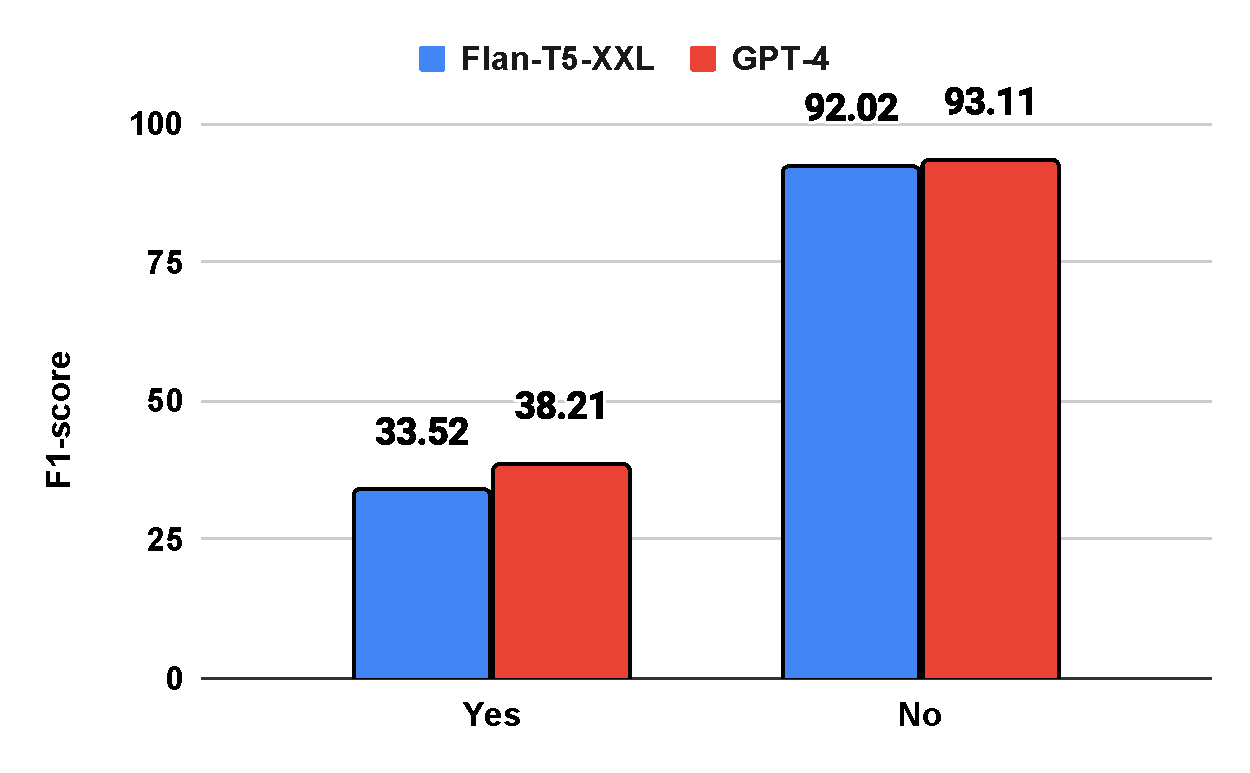
\includegraphics[width=\linewidth]{figures/gpt_4_flan_t5_xxl_social_message.pdf}
  \caption{F1-score for social message detection task class wise}
  \label{class_wise_social_message}
\end{subfigure}%
\begin{subfigure}{.50\textwidth}
  \centering
  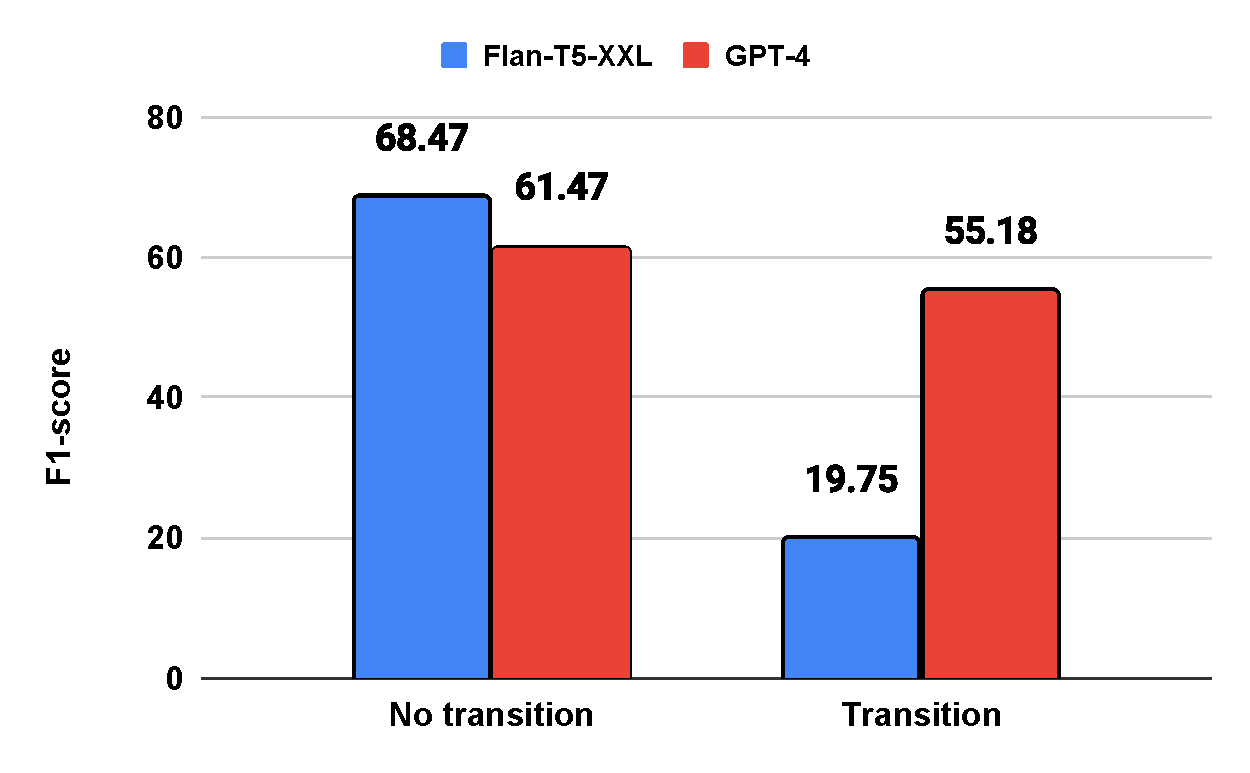
\includegraphics[width=\linewidth]{figures/gpt_4_flan_t5_xxl_transition.pdf}
  \caption{F1-score for tone transition detection task class wise}
  \label{class_wise_tone_transition}
\end{subfigure}
\caption{Comparisons between \texttt{Flan-T5-XXL} and \texttt{GPT-4} in terms of class-wise F1-score for the social message (Yes: Presence of social message, No: Absence of social message), Tone transition detection tasks.}
\label{tone_transition_social_message}
\end{figure}

\begin{figure}[h!]
    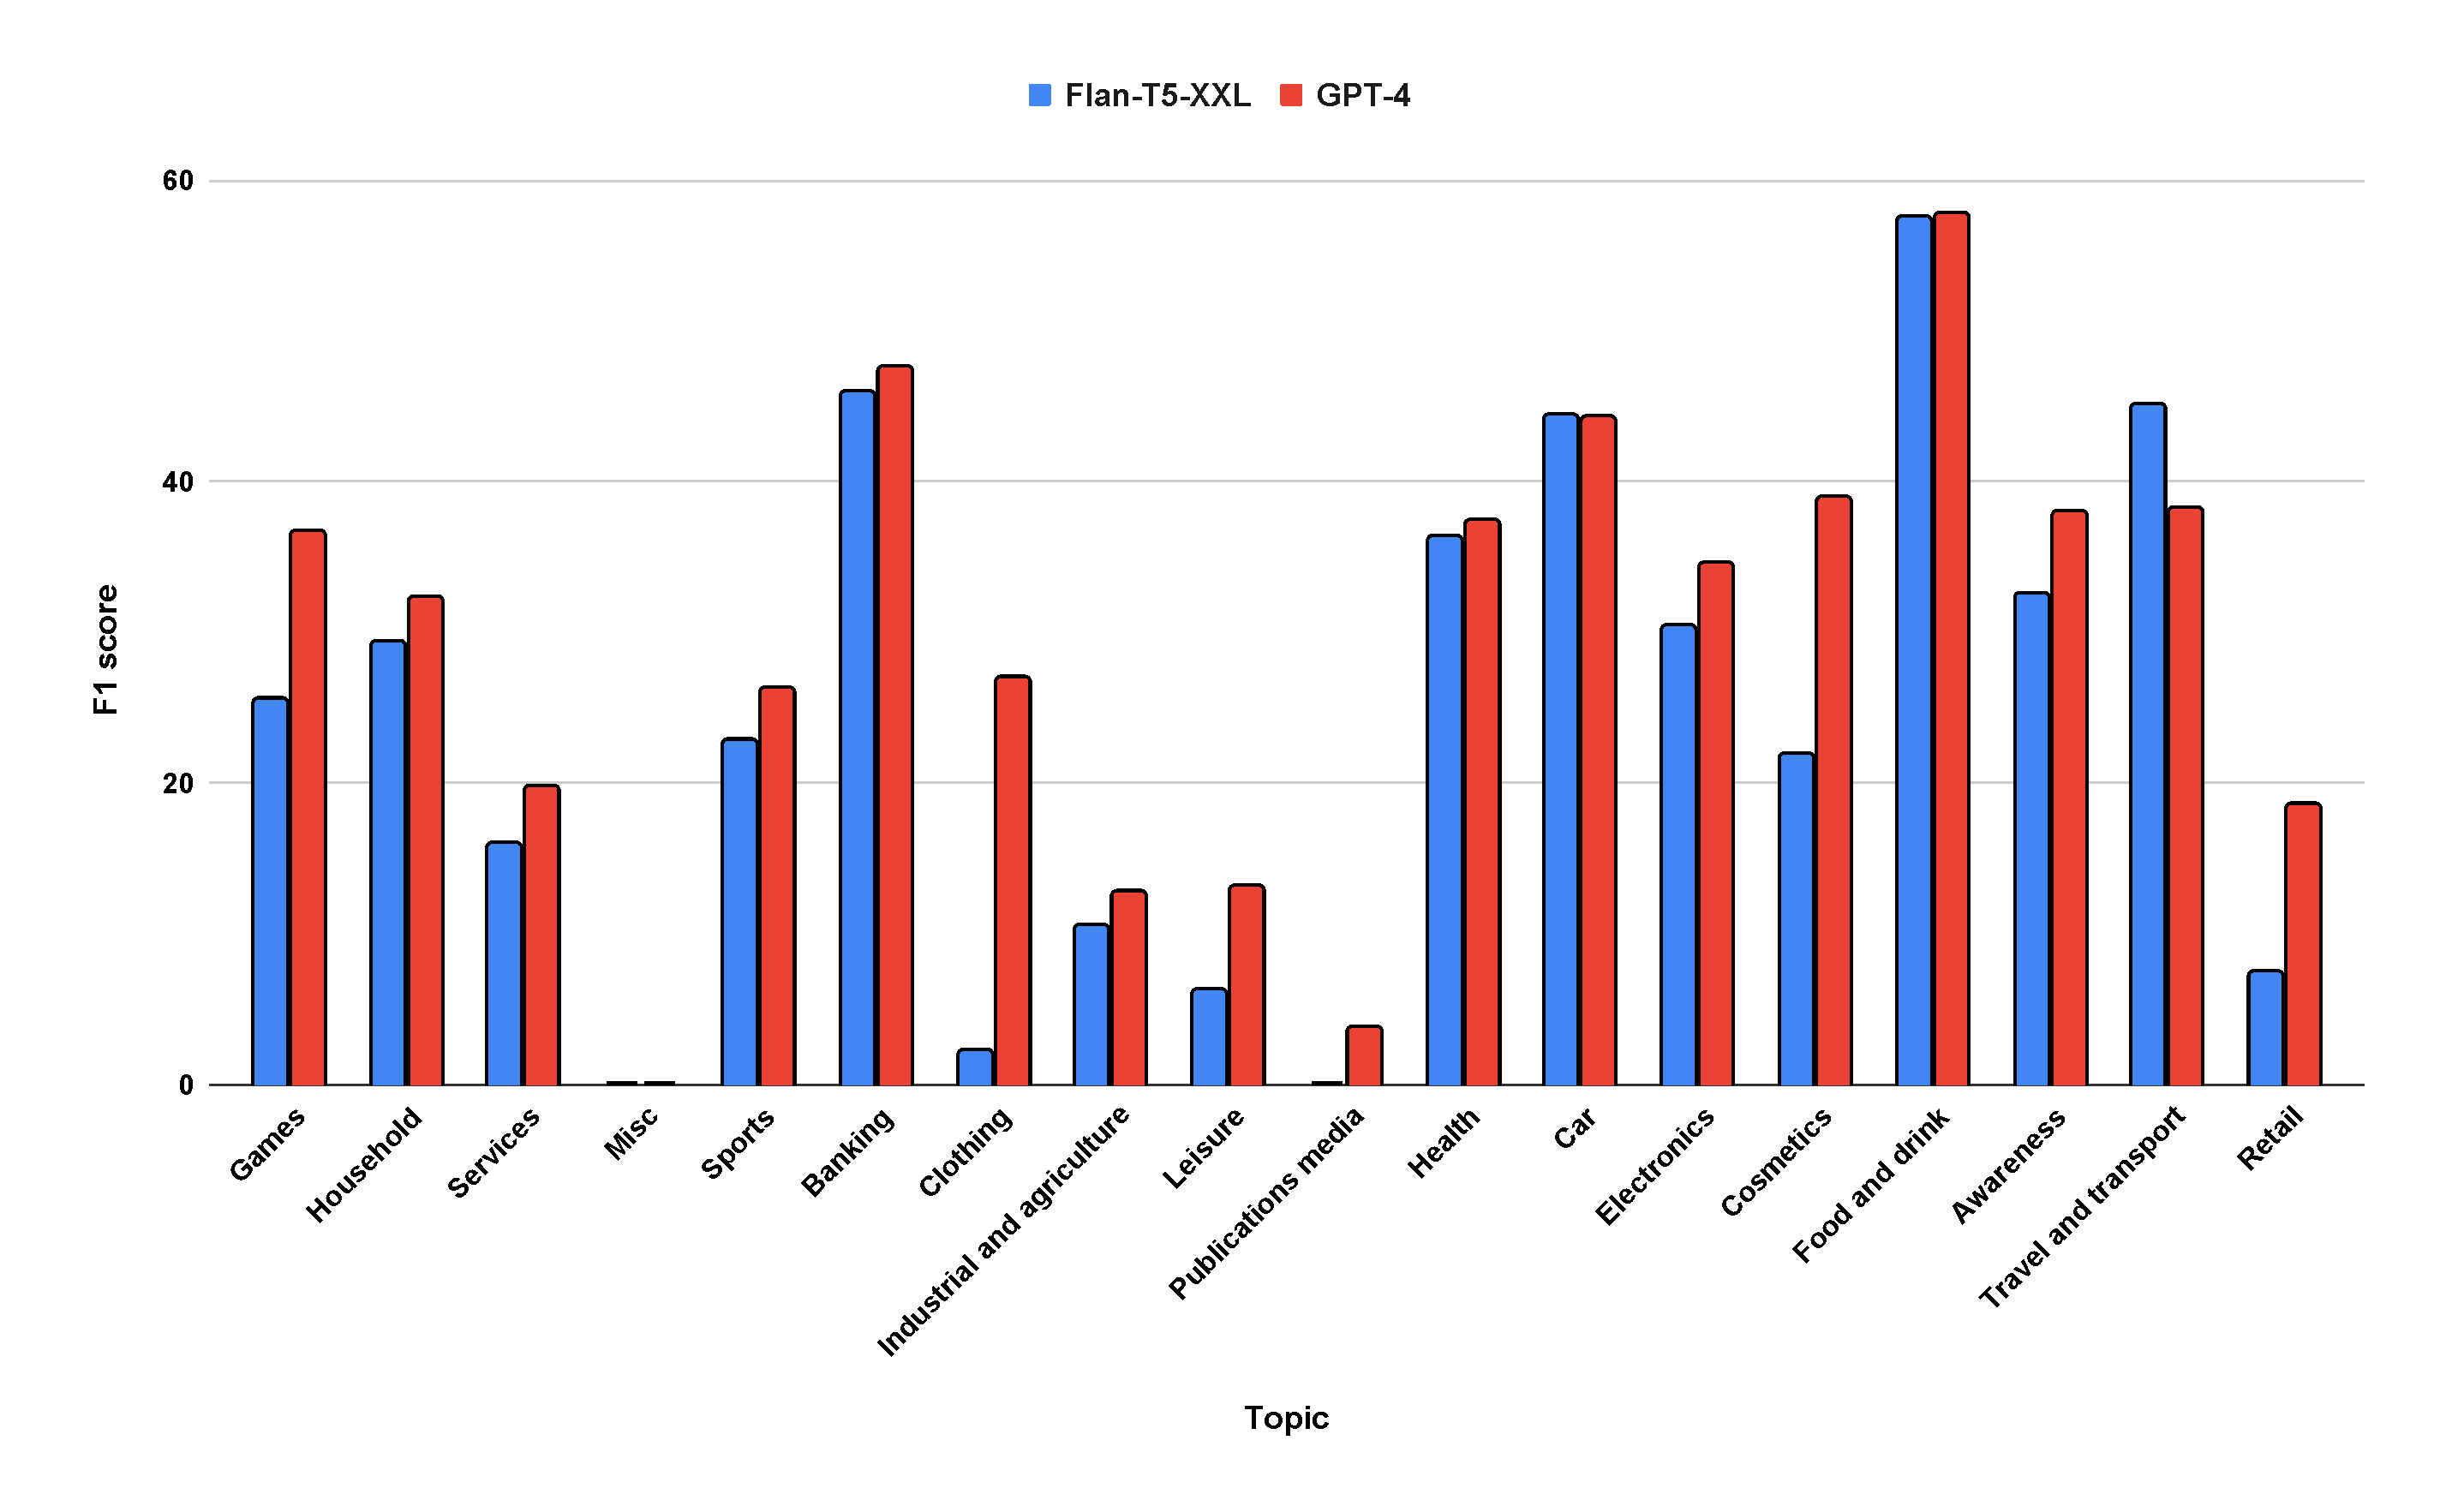
\includegraphics[width=\textwidth]{figures/gpt_4_flan_t5_xxl_topic.pdf}
    \caption{Comparisons between \texttt{Flan-T5-XXL} and \texttt{GPT-4} in terms of class-wise F1-score for the topic categorization task}
    \label{gpt_4_flan_t5_xxl_topic}
\end{figure}


\subsection{Unimodal vs Multimodal context fusion}

\begin{table}[h!]
\centering
\resizebox{\textwidth}{!}{
\begin{tabular}{|ccccccccc|}
\hline
\multicolumn{3}{|c|}{\textbf{Configurations}}                                                                               & \multicolumn{1}{c|}{\textbf{Acc}} & \multicolumn{1}{c|}{\textbf{F1}} & \multicolumn{1}{c|}{\textbf{Acc}} & \multicolumn{1}{c|}{\textbf{F1}} & \multicolumn{1}{c|}{\textbf{Acc}}   & \textbf{F1}  \\ \hline
\multicolumn{1}{|c|}{\textbf{Model}}      & \multicolumn{1}{c|}{\textbf{Features}} & \multicolumn{1}{c|}{\textbf{Modality}} & \multicolumn{2}{c|}{\textbf{Social message}}                         & \multicolumn{2}{c|}{\textbf{Tone transition}}                        & \multicolumn{2}{c|}{\textbf{Topic categorization}} \\ \hline
\multicolumn{1}{|c|}{\textbf{Random}}     & \multicolumn{1}{c|}{NA}                & \multicolumn{1}{c|}{NA}                & \multicolumn{1}{c|}{49.57±0.28}   & \multicolumn{1}{c|}{39.61±0.28}  & \multicolumn{1}{c|}{49.95±0.30}   & \multicolumn{1}{c|}{49.88±0.30}  & \multicolumn{1}{c|}{5.71±0.16}      & 4.71±0.24    \\ \hline
\multicolumn{1}{|c|}{\textbf{Majority}}   & \multicolumn{1}{c|}{NA}                & \multicolumn{1}{c|}{NA}                & \multicolumn{1}{c|}{90.96}        & \multicolumn{1}{c|}{47.63}       & \multicolumn{1}{c|}{54.11}        & \multicolumn{1}{c|}{35.11}       & \multicolumn{1}{c|}{23.04}          & 2.08         \\ \hline
\multicolumn{9}{|c|}{\textbf{Unimodal}}                                                                                                                                                                                                                                                                                        \\ \hline
\multicolumn{1}{|c|}{\textbf{LSTM}}       & \multicolumn{1}{c|}{CLIP-S}            & \multicolumn{1}{c|}{V}                 & \multicolumn{1}{c|}{90.57±0.47}   & \multicolumn{1}{c|}{68.65±1.70}  & \multicolumn{1}{c|}{61.93±0.37}   & \multicolumn{1}{c|}{61.65±0.37}  & \multicolumn{1}{c|}{52.86±0.43}     & 36.48±1.58   \\ \hline
\multicolumn{1}{|c|}{\textbf{MHA}}        & \multicolumn{1}{c|}{AST}               & \multicolumn{1}{c|}{A}                 & \multicolumn{1}{c|}{89.07±2.02}   & \multicolumn{1}{c|}{55.33±3.96}  & \multicolumn{1}{c|}{59.78±1.56}   & \multicolumn{1}{c|}{58.60±0.96}  & \multicolumn{1}{c|}{25.11±1.39}     & 15.48±1.57   \\ \hline
\multicolumn{1}{|c|}{\textbf{MHA}}        & \multicolumn{1}{c|}{CLIP-S}            & \multicolumn{1}{c|}{V}                 & \multicolumn{1}{c|}{90.41±2.24}   & \multicolumn{1}{c|}{72.28±1.66}  & \multicolumn{1}{c|}{61.74±1.07}   & \multicolumn{1}{c|}{61.48±1.11}  & \multicolumn{1}{c|}{61.30±0.89}     & 47.74±1.27   \\ \hline
\multicolumn{9}{|c|}{\textbf{Multimodal}}                                                                                                                                                                                                                                                                                      \\ \hline
\multicolumn{1}{|c|}{$\mathbf{Tx_{AT}}$}      & \multicolumn{1}{c|}{AST + BERT}        & \multicolumn{1}{c|}{A + T}             & \multicolumn{1}{c|}{90.24±0.81}   & \multicolumn{1}{c|}{64.02±0.81}  & \multicolumn{1}{c|}{62.98±0.56}   & \multicolumn{1}{c|}{62.29±0.83}  & \multicolumn{1}{c|}{42.99±0.65}     & 30.77±0.96   \\ \hline
\multicolumn{1}{|c|}{\textbf{(1) $\mathbf{Tx_{AV}}$}}  & \multicolumn{1}{c|}{CLIP-S +AST}       & \multicolumn{1}{c|}{A + V}             & \multicolumn{1}{c|}{91.62±0.58}   & \multicolumn{1}{c|}{70.05±0.67}  & \multicolumn{1}{c|}{64.01±0.54}   & \multicolumn{1}{c|}{63.72±0.66}  & \multicolumn{1}{c|}{61.62±0.46}     & 48.67±0.64   \\ \hline
\multicolumn{1}{|c|}{\textbf{(2) $\mathbf{Tx_{TV}}$}}  & \multicolumn{1}{c|}{CLIP-S +BERT}      & \multicolumn{1}{c|}{T + V}             & \multicolumn{1}{c|}{\textbf{92.23±0.57}}  & \multicolumn{1}{c|}{\textbf{74.03±1.00}}  & \multicolumn{1}{c|}{63.96±0.99}   & \multicolumn{1}{c|}{63.48±0.84}  & \multicolumn{1}{c|}{63.27±0.59}     & 50.58±1.32   \\ \hline
\multicolumn{1}{|c|}{\textbf{A-Max(1,2)}} & \multicolumn{1}{c|}{CLIP-S +BERT +AST} & \multicolumn{1}{c|}{A + V + T}          & \multicolumn{1}{c|}{92.51±0.46}   & \multicolumn{1}{c|}{73.17±1.00}  & \multicolumn{1}{c|}{\textbf{65.05±0.36}}   & \multicolumn{1}{c|}{\textbf{64.67±0.33}} & \multicolumn{1}{c|}{\textbf{65.92±0.54}}     & \textbf{54.22±1.14}  \\ \hline
\multicolumn{1}{|c|}{\textbf{D-Max(1,2)}} & \multicolumn{1}{c|}{CLIP-S +BERT +AST} & \multicolumn{1}{c|}{A + V + T}          & \multicolumn{1}{c|}{92.52±0.46}   & \multicolumn{1}{c|}{73.21±0.98}  & \multicolumn{1}{c|}{65.01±0.39}   & \multicolumn{1}{c|}{64.63±0.32}  & \multicolumn{1}{c|}{65.51±0.58}     & 53.67±1.24   \\ \hline
\end{tabular}
}
\caption{Comparative results between different unimodal and multimodal context fusion models across different tasks: Social message and Tone transition, Topic categorization. \textbf{\textit{\underline{CLIP-S}}}: Shot level features extracted using CLIP. \textbf{\textit{\underline{Modality:}}} A: Audio, V: Visual, T: Text. Results are reported as an average of 5 runs with randomly selected seeds. Best performing results are marked in bold for respective tasks.}  
\label{exptable}
\end{table}

From Table \ref{exptable}, we can see that supervised unimodal models (MHA, LSTM) show improved performance as compared to simple random and majority baselines. In terms of unimodal models, MHA model trained on shot-level visual features (denoted by CLIP-S) perform far better than audio features (AST) in social message detection (\textbf{F1: 72.28} vs \textbf{F1: 55.33}) and topic categorization tasks.
(\textbf{F1: 47.74} vs \textbf{F1: 15.48}). For the tone transition task, MHA model trained on audio features (AST) shows close performance (\textbf{F1:58.60} vs \textbf{F1: 61.48}) as compared to visual features, due to the dependence of the tone transition task on the ambient music. \\
For multimodal models, we observe that the fusion of text and visual modalities through a Perceiver-IO-based encoder ($\mathbf{Tx_{TV}}$) performs better (\textbf{F1:74.03}) for social message detection compared to audio-visual or audio-text fusion. This can be attributed to the presence of socially relevant descriptors in the transcripts and video shots. However, the fusion of audio with visual signals ($\mathbf{Tx_{AV}}$) improves the performance in the tone-transition detection task (\textbf{F1: 63.72}). For topic categorization, we find that the fusion of text and visual modalities ($\mathbf{Tx_{TV}}$) performs better than other paired modalities (\textbf{F1:50.58}) due to topic-specific identifiers in transcripts and shots. 
\par
 Our proposed approach based on logit fusion strategies: Average-Max (\textbf{A-Max}) and Dual-Max (\textbf{D-Max}) exhibits similar performance across all tasks. We obtain gain for tone-transition (\textbf{F1:64.67}) based on the \textbf{A-Max} fusion strategy of $\mathbf{Tx_{AV}}$ and $\mathbf{Tx_{TV}}$ models. In terms of class-wise metrics, \textbf{A-Max} fusion improves the transition class average F1-score to \textbf{61.28\%} as compared to $\mathbf{Tx_{AV}}$ (\textbf{60.72\%}) and $\mathbf{Tx_{TV}}$ (\textbf{60.18\%}). In the case of topic categorization, logit fusion through \textbf{A-Max} of $\mathbf{Tx_{AV}}$ and $\mathbf{Tx_{TV}}$ models results in the best performance (\textbf{F1: 54.22}). Further, \textbf{A-Max} fusion results in improvements over $\mathbf{Tx_{AV}}$ and $\mathbf{Tx_{TV}}$ across 15 topic categories (out of 18), with noticeable gains in the minority categories i.e., Retail ($\sim${\textbf{6.2\%}}), Industrial \& Agriculture ($\sim$\textbf{5\%}), Household ($\sim$\textbf{7\%}). Similar trends can be observed for \textbf{D-Max} fusion, with improvements obtained across 14 topic categories (out of 18).

\section{Limitations}
\section{Conclusions}






% More Research Topics
% \include{ResearchTopic2}

% Conclusion and ongoing work
\chapter{Conclusion and ongoing work}
\label{cha:conclusion}

Here, we would like to revisit the thesis statement before setting directions for ongoing/future work.

\begin{tcolorbox}[width=\textwidth]
Context-guided attention improves multi-modal content understanding at diverse scales.
\end{tcolorbox}


Till now, we have developed models based on context-guided attention for macro/instance level content understanding tasks w.r.t. domains of movies, TV shows, natural scenes, and advertisements. The content understanding tasks are reliant on the representations learned through context-guided attention mechanisms. Here, we would like to pose the following question regarding the enhancement of these learned representations:

\begin{itshape}
Q: Can we guide the representations learned through context-guided attention to be optimal yet robust for the given macro/instance level task?
\label{context:macro instance level}
\end{itshape}

In terms of guidance, we would like to consider the available knowledge from pretrained multimodal models. With the increase in web-based data sources, there is a trend toward the curation of large-scale weakly aligned datasets consisting of images/videos and noisy descriptions like LAION-5B \cite{schuhmann2022laionb}, CC-12M \cite{changpinyo2021cc12m}, WebVid \cite{Bain21}. The curation of these large-scale sources has led to the rise of multimodal pretraining \cite{wang2022MMPTMSurvey}, where transformer-based models are guided by certain objectives as follows:
\begin{itemize}

  \item \textbf{Image-text matching:} Detect whether the image and text pairs are aligned with each other  
 \item \textbf{Word-region alignment:} Detect whether certain words in the descriptions are matched to image regions
 \item \textbf{Caption generation:} Generate a natural language caption to match the given description with the image
 
\end{itemize}

The aforementioned pretraining tasks are certain examples of objectives used for large-scale models and by no means comprise an exhaustive list. The pretraining stage is followed by subsequent finetuning operations for a wide variety of downstream classification and generative tasks, as mentioned below:

\begin{itemize}

    \item \textbf{Classification tasks:} Visual-question answering, Video-language inference, Visual entailment, Category recognition, Multi-modal sentiment analysis
    \item \textbf{Generative tasks:} Image/Video captioning, Visual dialogue, Multimodal machine translation
    
\end{itemize}
 An outline of the pretraining and finetuning operation is shown in Fig \ref{multimodal pretraining}.

 \begin{figure}[h!]
    \centering
    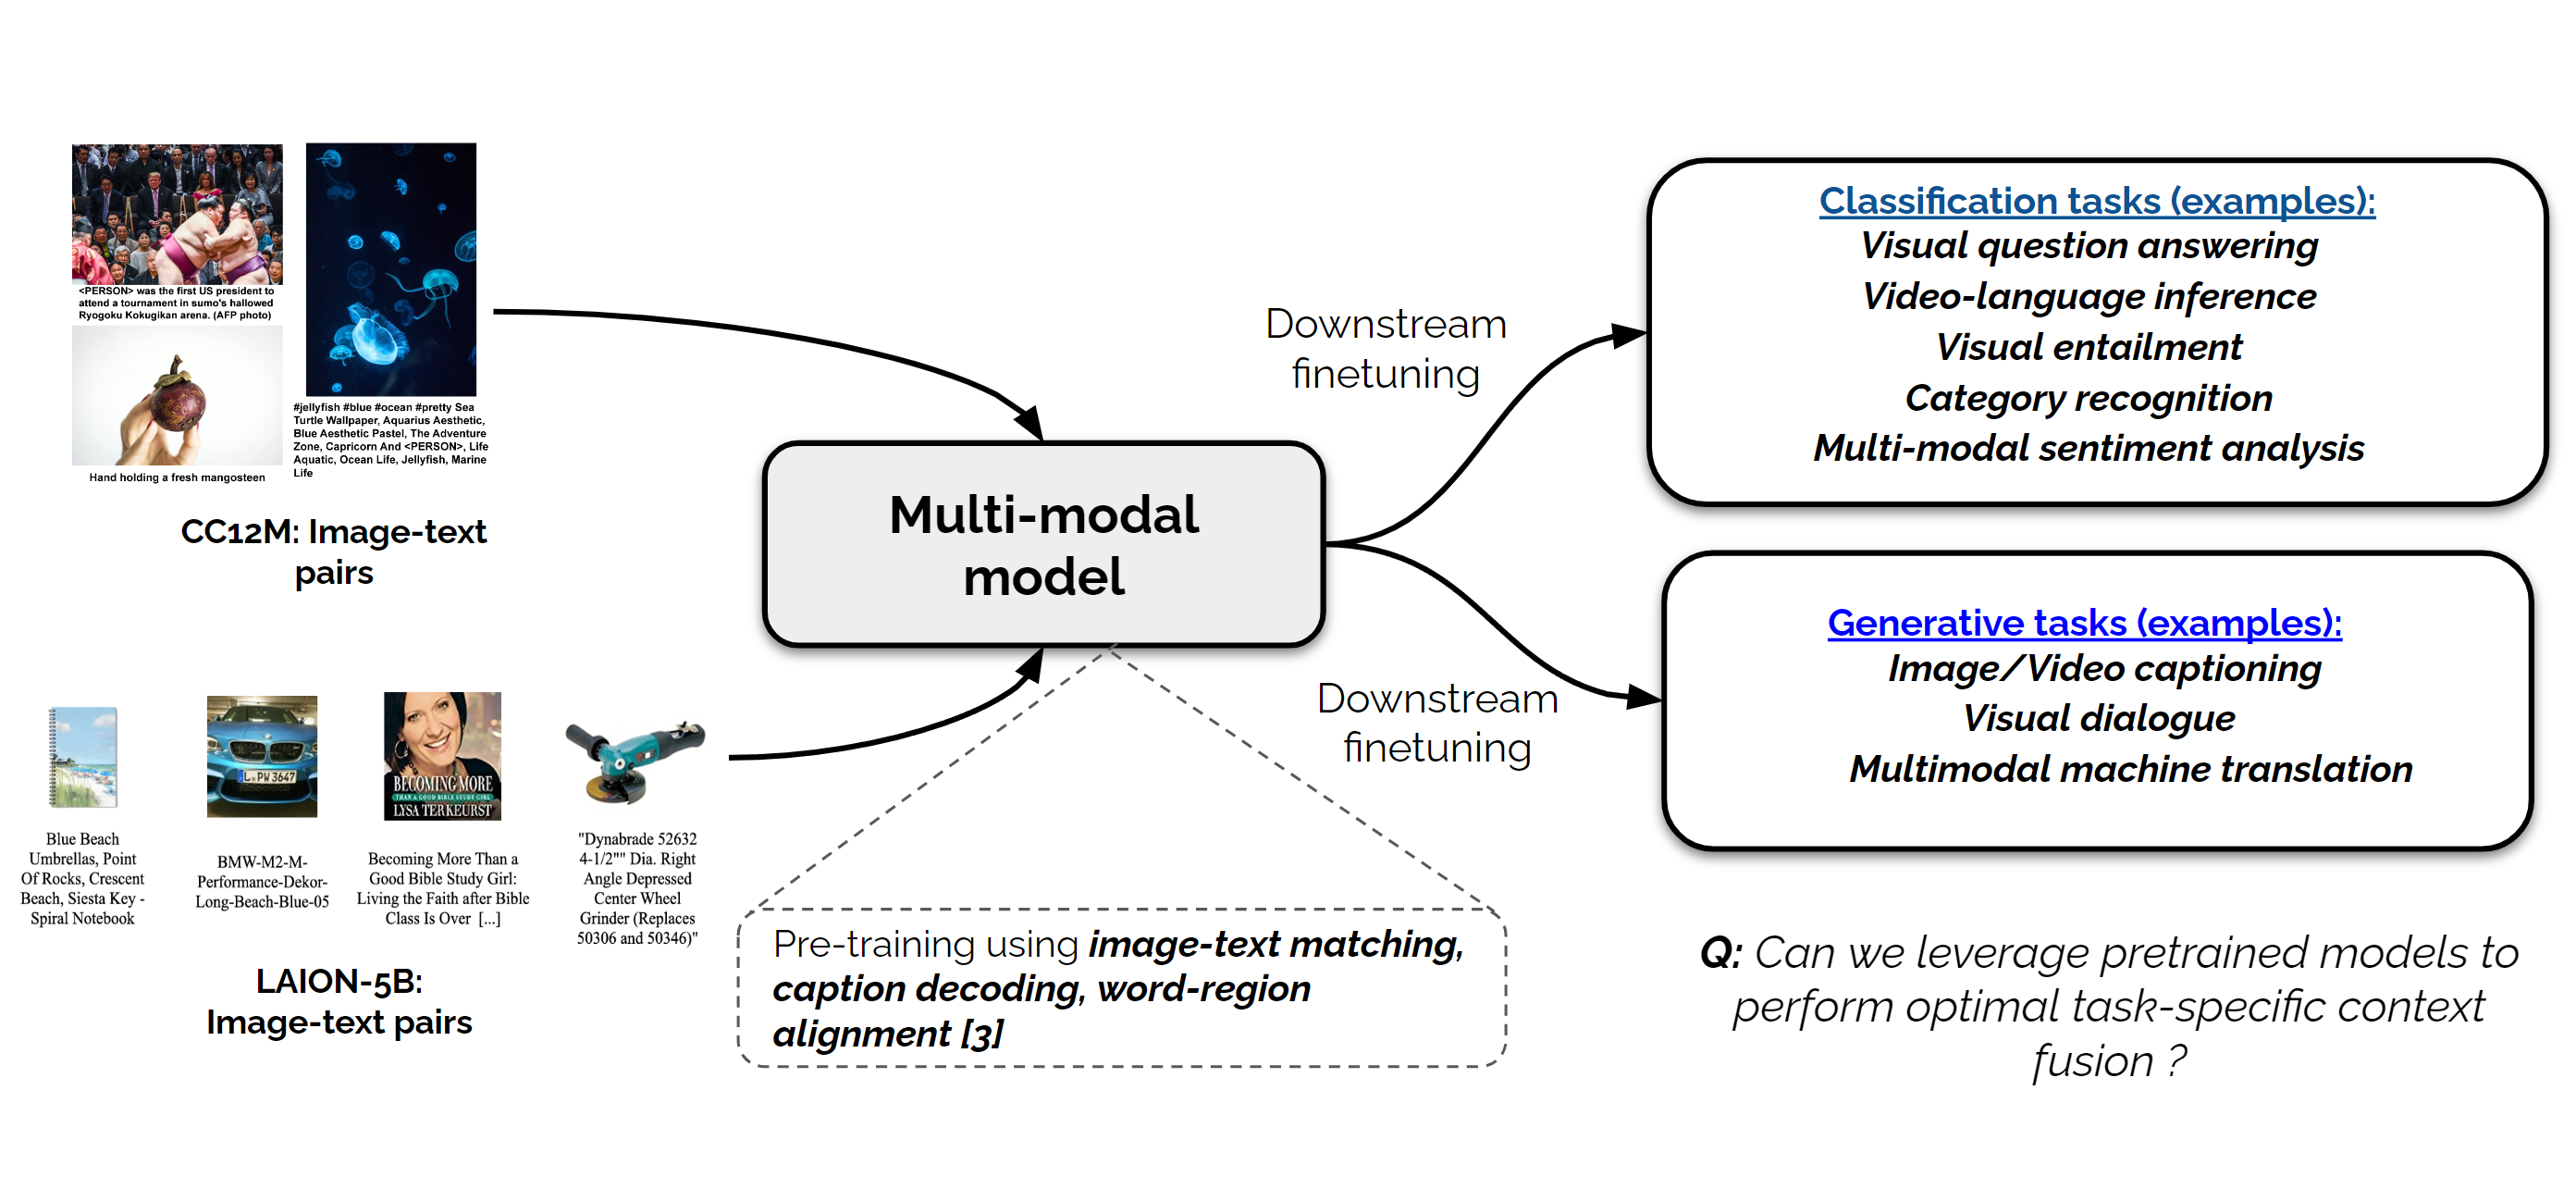
\includegraphics[width=\textwidth]{figures/multimodal_pretraining.png}
    \caption{Pretraining and finetuning operation pipeline in multimodal models.}
    \label{multimodal pretraining}
 \end{figure}

Hence we would like to recast the previous mentioned question to include the role of multimodal pretrained knowledge as follows:

\begin{itshape}
Q: Can we leverage existing large-scale multimodal knowledge to obtain optimal yet robust context-guided representations for given macro/instance-level tasks?
\end{itshape}

With this question, we introduce the concept of Information Bottleneck and how it can be used to obtain optimal yet robust representations for a given task.

\section{Information Bottleneck}

The information bottleneck principle \cite{Tishby2015DeepLA} formulates the goal of deep learning as a trade-off between compression and predictive power. If a given task has associated inputs $X$ and labels $Y$ and the intermediate layer representations of a deep learning model are denoted by $T$, then the optimal task-specific representation can be obtained through the following lagrangian formulation:

\begin{equation}
    L_{IB}= I(Y;T) - \beta I(X;T)
\end{equation}

Here, the objective aims at 
\begin{itemize}
    \item \textbf{Increasing predicting power:} Maximize the mutual information (MI) between labels $Y$ and representations $T$. 
    \item \textbf{Representation compression:} Minimize the mutual information (MI) between inputs $X$ and representations $T$.
\end{itemize}
The parameter $\beta$ controls the relative contributions of the two objective terms. In our case, we would like to explore the usage of information bottleneck as a regularization objective for pretrained multimodal models and its impact on macro and instance-level content understanding tasks under a variety of input settings. We outline our proposed work in the following sections:

\subsection{Related work}
Information Bottleneck (IB) has been utilized for low-resource finetuning of BERT for natural language inference and sentiment analysis tasks in \cite{Mahabadi2021VariationalIB}. Additional usage of information bottleneck includes its usage as task-specific regularizer for learning adversarially robust representations in language models \cite{wang2021infobert}. In the domain of multimodal learning, IB as a regularizer has enabled learning of multimodal representations robust to linguistic variations, image corruptions for visual question answering task \cite{Jiang2022CorrelationIB}. 

\subsection{Information bottleneck and multimodality}

\begin{figure}
     \centering
    \includegraphics[width=\textwidth]{figures/multimodal_IB.png}
    \caption{Multimodal architecture outline for information bottleneck.}
    \label{multimodal pretraining}
\end{figure}

The base multimodal pretrained architecture to be considered for information bottleneck-related study is shown in Fig \ref{multimodal pretraining} . Given two modalities $m_{1}$ and $m_{2}$, the sequence of operations can be listed as follows:

\begin{align}
    T_{m_{1}}&=f_{m_{1}}(X_{m_{1}}), T_{m_{2}}=f_{m_{2}}(X_{m_{2}})\\
    Y&=F_{m_{1}m_{2}}([T_{m_{1}},T_{m_{2}}])
\end{align}
Here $T_{m_{i}}$ refers to the input embeddings for modality $m_{i}$ and $F_{m_{1}m_{2}}$ refers to the multimodal encoder for predicting the labels. For the multimodal setting, the information bottleneck regularizer can be written as follows:

\begin{equation}
    L_{IB}= I(Y;\{T_{m_{1}},T_{m_{2}}\}) - \beta I(\{X_{m_{1}},X_{m_{2}}\};\{T_{m_{1}},T_{m_{2}}\})
\end{equation}

\subsection{Proposed work (A) - Optimal task-specific representations}
\label{Optimal task-specific representations}
In the first part of the proposed work, we would like to benchmark the performance of various multimodal models under the impact of information bottleneck for content understanding tasks. Since finetuning multimodal models is a memory-intensive operation, we would like to explore the parameter settings under which optimal task-specific representations can be extracted after using the information bottleneck as a regularizer. The outline of the proposed work can be found in Fig \ref{optimal_task_representations}.
The context-processing operation extracts contextual information from the given multimodal content through various modalities. The processed contextual information is passed as input to a pretrained multimodal model with a wide variety of parameter settings:
\begin {itemize}
\item \textbf{Linear-Probe:} Finetuning of the task-specific classifier head only and complete freezing of the multimodal encoder.
\item \textbf{Parameter efficient techniques:} Usage of parameter efficient techniques like LoRA, Adapters, prefix tuning for the multimodal encoder
\item \textbf{Full finetuning:} Complete finetuning of the multimodal encoder.
\end{itemize}
For the above parameter settings, we would like to investigate the impact of information bottleneck guidance while finetuning for a host of macro and instance-level tasks as follows:

\begin{itemize}
    \item \textbf{Advertisement video understanding:} Proposed MM-AU Benchmark
    \item \textbf{Hateful content detection:} Hateful memes \cite{Kiela2020TheHM} dataset
    \item \textbf{Movie understanding:}  Movie genre classification \cite{2019Moviescope}, MMIMDB \cite{Arevalo2017GatedMU}
    \item \textbf {Human affect understanding:} Emotic \cite{kostiPAMI}, CAER \cite{CAER-S}
\end{itemize}
\begin{figure}
 \centering 
 \includegraphics[width=\textwidth]{figures/optimal_task_representations.png}
 \caption{Optimal macro and instance-level task representations based on information bottleneck under different parameter settings}
 \label{optimal_task_representations}
\end{figure}

In terms of architecture, we plan to use the following based on different modality combinations:
\begin{itemize}
\item \textbf{Vision-language:} BLIP-2 \cite{Li2023BLIP2BL}, ViLT \cite{Kim2021ViLTVT}
\item \textbf{Audio-visual:} UAVM model \cite{uavm_gong}
\end{itemize}


\subsection{Proposed work (B) - Characterizing robustness}

Our previous approaches regarding macro and instance level content understanding relied on the assumption that the input sources are free from corruption. However, in real-life settings, the modalities associated with input sources undergo corruption as mentioned in the following examples:

\begin{itemize}
 \item \textbf{Acquisition failure:}  Failure of camera sensors in traffic intersections.
 \item \textbf{Privacy concerns:} Privacy restrictions on accessing social media posts or chats.
 \item \textbf{Noise corruptions:} Excessive noise in audio recordings to be used for emotion classification
\end{itemize}

In the second part of our proposed work, we plan to use the information bottleneck regularizer under the settings of corrupted modalities for pretrained multimodal models. The overall goal is to determine the robustness of the pretrained models with and without information bottleneck regularizer during finetuning. An outline of the corrupted modality setting with our previous optimal task-specific representation framework based on information bottleneck (IB) is shown in Fig \ref{robustness_multimodal_models}.

\begin{figure}
 \centering 
 \includegraphics[width=\textwidth]{figures/robustness_multimodal_models.png}
 \caption{Optimal macro and instance-level task representations based on information bottleneck under different parameter settings}
 \label{robustness_multimodal_models}
\end{figure}

We plan to consider the following training and testing scenarios in the robustness study setting:

\begin{itemize}

\item \textbf{Scenario A:} Finetune multimodal model under different parameter settings with IB regularizer and non-corrupted modality inputs.
\item \textbf{Scenario B:} Finetune multimodal model under different parameter settings with IB regularizer and corrupted modality inputs
\item \textbf{Scenario C:} Finetune multimodal model under different parameter settings with IB regularizer and mutual information (MI) maximization between non-corrupted inputs and multimodal representations.

\end{itemize}

In the above-mentioned scenarios, the evaluation will be performed using corrupted modality data. We plan to use the datasets and architectures mentioned in the previous section for this study as well. 


% Using single-space for reference list.
\begin{singlespace}
% Bibliography
\phantomsection
\addcontentsline{toc}{chapter}{References}%
\markboth{References}{References}%
% If you use BibLaTeX
\printbibliography[title=References]
% If you use BibTeX
% \bibliographystyle{plain}
% \bibliography{references}
\end{singlespace}

% Appendices
\phantomsection
\addcontentsline{toc}{chapter}{Appendices}%
\markboth{Appendices}{Appendices}%
\chapter*{Appendices}
\renewcommand\thesection{\Alph{section}}
\renewcommand*{\thesubsection}{\Alph{section}.\arabic{subsection}}
\begingroup
\numberwithin{equation}{section}
% Appendix source files
\section{MovieCLIP dataset}
\label{app:scene_categories}

\subsection{Scene classes distribution wrt sources}
Here \textbf{Movie Slugline} refers to the set of labels obtained exclusively from sluglines in movie scripts. \textbf{Common Label} refers to the set of common labels between taxonomy considered in \textbf{HVU} \cite{diba_large_2020} and \textbf{Movie Slugline}. Here \textbf{HVU} \cite{diba_large_2020} refers to the set of labels obtained exclusively from the taxonomy used for curating \textbf{HVU} \cite{diba_large_2020} dataset. \textbf{Human expert} refers to the set of labels added by the human expert during the taxonomy refinement procedure.

\begin{itemize}
    \item \textbf{Movie Slugline:} \textit{tent}, \textit{computer room}, \textit{truck}, \textit{study},
 \textit{gas station}, \textit{cafe}, \textit{shuttle}, \textit{courthouse}, \textit{elevator}, \textit{tower}, \textit{dorm}, \textit{station}, \textit{club}, \textit{lobby}, \textit{mall}, \textit{salon}, \textit{prison}, \textit{bus}, \textit{stairs}, \textit{theater}, \textit{car}, \textit{booth}, \textit{locker room}, \textit{hangar}, \textit{closet},
 \textit{farmhouse}, \textit{post office}, \textit{townhouse}, \textit{ship}, \textit{loft}, \textit{yard}, \textit{zoo}, \textit{funeral}, \textit{art gallery}, \textit{castle}, \textit{subway}, \textit{lounge}, \textit{train}, \textit{morgue}, \textit{museum}, \textit{wagon}, \textit{manor}, \textit{mansion}, \textit{library}, \textit{pool}, \textit{cellar}, \textit{cab}, \textit{safe house}, \textit{classroom}, \textit{helicopter}, \textit{police station}, \textit{courtroom}, \textit{city hall}, \textit{fire station}, \textit{corridor}, \textit{control room}, \textit{airport}, \textit{cabin}, \textit{war room}, \textit{plane}, \textit{press room}, \textit{cottage}, \textit{residence}, \textit{penthouse}, \textit{inn}, \textit{church}, \textit{suburban}, \textit{interrogation room}, \textit{conference room}

 \item \textbf{Common label:} \textit{tunnel, bakery, shack, building, baseball field, hotel, desert, factory, bathroom, downtown, restaurant, village, playground, boxing ring, gym, bridge, beach, workshop, cave, clinic, arena, garden, stage, office, attic, bowling alley, apartment, deck, cockpit, dining room, basketball court, grove, ballroom, forest, house, barn, alley, park, bay, golf course, chapel, home, parking, bar, kitchen, school, swamp, basement, walkway, bedroom, garage, lake, bank, living room, room,
 auditorium, street, valley, casino, hall, waterfall, warehouse,
 tennis court, farm, hospital, palace, estate, river}
 
 \item \textbf{HVU:} \textit{archaeological site, shore,
 batting cage, animal shelter, plaza, hot spring,
 harbor, bullring, sandbank, town, mountain,
 retail, courtyard, sea, road, shooting range,
 pond, stadium, foundry, skyline, amusement park,
 market, laboratory, race track, kindergarten, ice rink}

\item \textbf{Human expert:} \textit{agriculture field, makeup studio, grassland, construction site,
 graveyard, automotive repair, overpass, studio, boat, fair, balcony, battlefield, banquet, phone booth,
 concert hall, meadow}
\end{itemize}

\section{MM-AU Benchmark}
\label{app:topic_categories}
\subsection{Topic categories}

We provide the mapping between Cannes(CC) \cite{cannes-lions}, Ads of the World (AOW)\footnote{https://www.adsoftheworld.com/} and Video-Ads (VA) \cite{Hussain2017AutomaticUO} coding schemes for obtaining the final set of topic categories as follows:

\begin{itemize}
    \item \textbf{Games:} Games and toys [\textcolor{blue}{\textbf{VA}}]; Gaming [\textcolor{red}{\textbf{AOW}}]
    \item \textbf{Household:} Household: Home Appliances, Furnishing [\textcolor{purple}{\textbf{CC}}]; Cleaning products, Home improvements and repairs, Home appliances [\textcolor{blue}{\textbf{VA}}]
    \item \textbf{Services:} Other services i.e. dating, tax, legal, loan, religious, printing, catering, etc. [\textcolor{blue}{\textbf{VA}}]; Professional Services [\textcolor{red}{\textbf{AOW}}].
    \item \textbf{Misc:} Miscellaneous, Business equipment and services [\textcolor{purple}{\textbf{CC}}]; Petfood, Political candidates (Politics) [\textcolor{blue}{\textbf{VA}}]; Pets [\textcolor{red}{\textbf{AOW}}]
    \item \textbf{Sports:} Sports equipment and activities [\textcolor{blue}{\textbf{VA}}]; Sports [\textcolor{red}{\textbf{AOW}}]
    \item \textbf{Banking:} Banking and services [\textcolor{purple}{\textbf{CC}}]; Financial services [\textcolor{blue}{\textbf{VA}}]; Finance [\textcolor{red}{\textbf{AOW}}]
    \item \textbf{Clothing:} Clothing, Footwear \& Accessories [\textcolor{purple}{\textbf{CC}}]; Clothing and accessories [\textcolor{blue}{\textbf{VA}}]; Personal Accessories [\textcolor{red}{\textbf{AOW}}] 
    \item \textbf{Industrial and agriculture:} Industrial, Agriculture Public Interest, Agriculture Professional Services [\textcolor{red}{\textbf{AOW}}]
    \item \textbf{Leisure:} Entertainment \& Leisure [\textcolor{purple}{\textbf{CC}}]; Gambling (lotteries, casinos, etc.) [\textcolor{blue}{\textbf{VA}}]; Recreation, Gambling [\textcolor{red}{\textbf{AOW}}]
    \item \textbf{Publications \& media:} Media \& Publications  [\textcolor{purple}{\textbf{CC}}]; Media and arts [\textcolor{blue}{\textbf{VA}}]; TV Promos, Music, Media, Movies [\textcolor{red}{\textbf{AOW}}]
    \item \textbf{Health:} Healthcare \& Pharmacy [\textcolor{purple}{\textbf{CC}}]; Health care and medications [\textcolor{blue}{\textbf{VA}}]; Health, Pharmaceutical [\textcolor{red}{\textbf{AOW}}]
    \item \textbf{Car:} Cars \& Automotive Products \& Services [\textcolor{purple}{\textbf{CC}}]; Car [\textcolor{blue}{\textbf{VA}}]; Automotive [\textcolor{red}{\textbf{AOW}}]
    \item \textbf{Electronics:} Home electronics and audio-visual [\textcolor{purple}{\textbf{CC}}]; Electronics, Phone, TV and internet service providers [\textcolor{blue}{\textbf{VA}}]; Electronics [\textcolor{red}{\textbf{AOW}}]
    \item \textbf{Cosmetics:} Cosmetics \& Toiletries [\textcolor{purple}{\textbf{CC}}]; Beauty products and cosmetics, Baby products [\textcolor{blue}{\textbf{VA}}]; Beauty [\textcolor{red}{\textbf{AOW}}]
    \item \textbf{Food and drink:} Savoury Foods, Sweet Foods \& Snacks, Non Alcoholic drinks, Alcoholic drinks [\textcolor{purple}{\textbf{CC}}]; Chocolate, Chips, Seasoning, Coffee, Soda, juice, milk, energy drinks, water, Alcohol [\textcolor{blue}{\textbf{VA}}]; Food, Non-Alcoholic Drinks, Confectionery, Alcoholic drinks [\textcolor{red}{\textbf{AOW}}]
    \item \textbf{Awareness:} Charities and non-profit [\textcolor{purple}{\textbf{CC}}]; Environment, Animal rights, Human rights, Safety, Smoking, Alcohol Abuse, Domestic Violence, Self-esteem, cyberbullying [\textcolor{blue}{\textbf{VA}}]; Education, Agency Self-Promo [\textcolor{red}{\textbf{AOW}}]
    \item \textbf{Travel and transport:} Travel \& Transport [\textcolor{purple}{\textbf{CC}}]; Vacation and travel [\textcolor{blue}{\textbf{VA}}]; Transport, Hospitality [\textcolor{red}{\textbf{AOW}}]
    \item \textbf{Retail:} Retail \& e-commerce [\textcolor{purple}{\textbf{CC}}]; Shopping (department stores, drug stores, groceries, etc.) [\textcolor{blue}{\textbf{VA}}]; Retail Services [\textcolor{red}{\textbf{AOW}}]
\end{itemize}
The taxonomy sources are listed within [.] for respective subcategories for the final list of topic categories. 


\section{MM-AU Experiments}
\label{app:language_baselines}
\subsection{Language based reasoning}

We investigate the zero-shot performance of several large language models i.e. \texttt{GPT-4}\cite{OpenAI2023GPT4TR}, \texttt{Opt-IML} \cite{Iyer2022OPTIMLSL}, \texttt{Flan-T5} (XXL,XL,L) \cite{Chung2022ScalingIL} and \texttt{Alpaca} \cite{alpaca} on the benchmark tasks associated with \textbf{MM-AU} dataset. For zero-shot evaluation, we report the results on 1670 non-empty transcripts out of the test split of 1692 samples.
\subsubsection{Flan-T5:}
For \texttt{Flan-T5}, we use the following prompts for the social message (\textbf{SM}), tone transition (\textbf{TT}), topic categorization(\textbf{Topic}) tasks: 
\begin{itemize}

\item \textbf{\underline{TT:}} 
\texttt{<Text from transcript>} \\
\textit{Based on the given text transcript from the advertisement, determine if the advertisement has any transitions in tones.} \\ 
\textbf{OPTIONS:}
\begin{itemize}
\item[-] Transition
\item[-] No transition
\end{itemize}
\textbf{ANSWER:}

\item \textbf{\underline{SM:}}
\texttt{<Text from transcript>} \\
\textit{An advertisement video has a social message if it provides awareness about any social issue. Examples of social issues: gender equality, drug abuse, police brutality, workplace harassment, domestic violence, child labor, environmental damage, homelessness, hate crimes, racial inequality etc. Based on the given text transcript, determine if the advertisement has any social message.}\\
\textbf{OPTIONS:}
\begin{itemize}
\item[-] Yes
\item[-] No
\end{itemize}
ANSWER: 

\item \textbf{\underline{Topic:}}
\texttt{<Text from transcript>} \\
\textit{Associate a single topic label with the transcript from the given set:} \\
\textbf{OPTIONS:}
\begin{itemize}
\item [-] Games
\item [-] Household
\item [-] Services
\item [-] Sports 
\item [-] Banking 
\item [-] Clothing 
\item [-] Industrial and agriculture 
\item [-] Leisure 
\item [-] Publications media 
\item [-] Health 
\item [-] Car 
\item [-] Electronics 
\item [-] Cosmetics 
\item [-] Food and drink 
\item [-] Awareness 
\item [-] Travel and transport 
\item [-] Retail 
\end{itemize}
\textbf{ANSWER:}
\end{itemize}

\subsubsection{OPT:} For \texttt{OPT}, we use the following prompt templates for different tasks:

\begin{itemize}

    \item \textbf{\underline{TT:}} \textit{Instruction: In this task, you are given a transcription of an advertisement, determine if the advertisement has any transitions in tones.} \\
    \textbf{Transcription:} \texttt{<Text from transcript>}\\
    \textbf{OPTIONS:}
    \begin{itemize}
    \item[-] Transition
    \item[-] No transition
    \end{itemize}
   \textbf{Answer:}

    \item \textbf{\underline{SM:}} \textit{In this task, you are given a transcription of an advertisement. An advertisement video has a social message if it provides awareness about any social issue. Example of social issues: gender equality, drug abuse, police brutality, workplace harassment, domestic violence, child labor, environmental damage, homelessness, hate crimes, racial inequality etc. Your task is to give label "Yes" if the advertisement given has any social message, otherwise give label "No".} \\
    \textbf{Transcription:} \texttt{<Text from transcript>}\\
    \textbf{Answer:}
    
    \item \textbf{\underline{Topic:}} \textit{In this task, you are given a transcription of an advertisement. Your task is to associate a single topic label with the transcript from the given set.} \\
    \textbf{Transcription:} \texttt{<Text from transcript>}\\
    \textbf{OPTIONS:}
    \begin{itemize}
    \item [-] Games
    \item [-] Household
    \item [-] Services
    \item [-] Sports 
    \item [-] Banking 
    \item [-] Clothing 
    \item [-] Industrial and agriculture 
    \item [-] Leisure 
    \item [-] Publications media 
    \item [-] Health 
    \item [-] Car 
    \item [-] Electronics 
    \item [-] Cosmetics 
    \item [-] Food and drink 
    \item [-] Awareness 
    \item [-] Travel and transport 
    \item [-] Retail 
    \end{itemize}
    \textbf{Answer:}
\end{itemize}

\subsubsection{alpaca:} 
For \texttt{alpaca}, we use the following prompt templates for different tasks:

\begin{itemize}
    \item \textbf{\underline{TT:}} \textit{Instruction: In this task, you are given a transcription of an advertisement determine if the advertisement has any transitions in tones.}\\
\textbf{Transcription}: \texttt{<Text from transcript>}\\
\textbf{Options:}
\begin{itemize}
\item[-] Transition
\item[-] No transition
\end{itemize}
\textbf{Answer:}
\item \textbf{\underline{SM:}} \textit{Instruction: In this task, you are given a transcription of an advertisement. An advertisement video has a social message if it provides awareness about any social issue. Example of social issues: gender equality, drug abuse, police brutality, workplace harassment, domestic violence, child labor, environmental damage, homelessness, hate crimes, racial inequality etc. Based on the given text transcript, determine if the advertisement has any social message. }\\
    \textbf{Transcription:} \texttt{<Text from transcript>}\\
\textbf{Options:}
\begin{itemize}
\item[-] Yes
\item[-] No
\end{itemize}
\textbf{Answer:}
\item \textbf{\underline{Topic:}} \textit{Instruction: In this task, you are given a transcription of an advertisement. Your task is to associate a single topic label with the transcript from the given set.}\\
\textbf{Transcription:} \texttt{<Text from transcript>}\\
\textbf{Options:}
    \begin{itemize}
    \item [-] Games
    \item [-] Household
    \item [-] Services
    \item [-] Sports 
    \item [-] Banking 
    \item [-] Clothing 
    \item [-] Industrial and agriculture 
    \item [-] Leisure 
    \item [-] Publications media 
    \item [-] Health 
    \item [-] Car 
    \item [-] Electronics 
    \item [-] Cosmetics 
    \item [-] Food and drink 
    \item [-] Awareness 
    \item [-] Travel and transport 
    \item [-] Retail 
\end{itemize}
\textbf{Answer:}
\end{itemize}
For \texttt{GPT-4} we use the recently released API to pass the prompts for individual tasks.
For \texttt{Flan-T5} and \texttt{Opt-IML}, we use the publicly available models as a part of Huggingface \cite{wolf-etal-2020-transformers} library. For \texttt{alpaca}, we use the publicly available implementation in Github \cite{alpaca}. The large language models sometimes assign a label to the prediction that does not lie within the set of valid labels for the respective tasks. In the case of those samples, we randomly assign a label from the task-specific label taxonomy. 

\endgroup

% In case your dissertation has multiple volumes.
% \addvolumecontents{thesis_part2}
% \addvolumecontents{thesis_part3}
% \addvolumecontents[lof]{thesis_part2}

\end{document}
